%!TEdddX TS-program = latex
% !TEX useTabs
%!TEX encoding = UTF-8 Unicode
% !BIB TS-program = biber
% !BIB program = biber
%%%%%%%%%%%%%%%%%%%%%%%%%%%%%%%%%%%%%%%%%
% 
% CC BY-NC-SA 3.0 (http://creativecommons.org/licenses/by-nc-sa/3.0/)
%
%%%%%%%%%%%%%%%%%%%%%%%%%%%%%%%%%%%%%%%%%

\documentclass{BYUTextbookRMM} 
\sloppy									% stop the complaining!
%----------------------------------------------------------------------------------------
%!TEX root =  main.tex

\usepackage{multirow}

\usepackage{geometry} % 
    \setlength{\marginparwidth}{2in}
    \setlength{\marginparsep}{0.25in}
    \setlength{\oddsidemargin}{0.0in}
    \setlength{\evensidemargin}{1.5in}
    \setlength{\textwidth}{5in}
    \setlength{\topmargin}{0in}
    \setlength{\headheight}{0.2in}
    \setlength{\headsep}{0.35in}
    \setlength{\textheight}{8.4in}
    \setlength{\footskip}{0.35in}
    \setlength{\columnsep}{0.35in}
    \raggedbottom
    \renewcommand{\baselinestretch}{1}

%
% Graphics
%
\usepackage{tikz}
\usetikzlibrary{arrows,automata,positioning,shapes.geometric,fit,calc,matrix,spy}
\usepackage{pgfplots}
\pgfplotsset{compat=1.13}

\usepackage{svg}
%
% Fonts
%
\usepackage[utf8]{inputenc} 	% Required for including letters with accents

%
% Math
%

\usepackage{polynom}		%polynomial long division
\usepackage{mathdots}		% in order to get \iddots

%----------------------------------------------------------------------------------------
%	GLOSSARY
%----------------------------------------------------------------------------------------

\usepackage[xindy,toc,section=chapter]{glossaries}
\makeglossaries
\renewcommand*{\glstextformat}{\textbf}



%----------------------------------------------------------------------------------------
%	BIBLIOGRAPHY 
%----------------------------------------------------------------------------------------

\usepackage{csquotes}
\usepackage[style=alphabetic,citestyle=numeric,sorting=nyt,sortcites=true,autopunct=true,autolang=hyphen,hyperref=true,abbreviate=false,backref=true,backend=biber]{biblatex}
\addbibresource{ch00/bibliography.bib} % BibTeX bibliography file
\defbibheading{bibempty}{}




\newglossaryentry{translation}
{
	name={translation},
	description={the transformation that shifts a graph (without distortion) some finite distance in the plane or space}
}
\newglossaryentry{pre-image}
{
	name={pre-image},
	description={The original function or relation, before it under goes transformations and become an image}
}
\newglossaryentry{image}
{
	name={image},
	description={A transformed version of the original function or relation}
}
\newglossaryentry{asymptote}
{
	name={asymptote},
	description={A shape that the graph of function approaches and gets arbitrarily close to on some open interval}
}
\newglossaryentry{periodic}
{
	name={periodic},
	description={Repeating on some regular interval, called the period}
}
\newglossaryentry{linear}
{
	name={linear},
	description={An algebraic function, equivalent to a polynomial of degree 1.  The general equation is $ax+b$, where $a$ and $b$ are constants.  The graph is a straight line.  The numerical data displays an add-add pattern.  Verbally, one variable is directly proportional to another, but with a potentially different starting point}
}
\newglossaryentry{quadratic}
{
	name={quadratic},
	description={An algebraic function, equivalent to a polynomial of degree 2.  The general equation is $ax^2+bx+c$, where $a,b,c$ are constants and $a\ne0$.  The graphical shape is called a parabola.  The numerical data displays an add-second difference pattern.  Verbally, one variable is directly proportional to the square of another}
}
\newglossaryentry{exponential}
{
	name={exponential},
	description={A transcendental function, where the independent variable appears as an exponent.  An untranslated, general equation form is $a\cdot{}b^x$, where $a$ and $b$ are constants}
}
\newglossaryentry{logarithm}
{
	name={logarithm},
	description={The inverse of an exponential function.  $y=\log_a{x}$ is equivalent to $a^y=x$}
}
\newglossaryentry{closure}
{
	name={closure},
	description={The quality of some operations over certain sets, that performance of that operation on members of the set always produces a member of the same set}
}
\newglossaryentry{transcendental}
{
	name={transcendental},
	description={Not algebraic.  That is, not derived from a polynomial with whole number exponents and rational coefficients}
}
\newglossaryentry{irrational numbers}
{
	name={irrational numbers},
	description={Numbers that cannot be represented as a ratio integers.  When written as a decimal, the digits are non-repeated and non-terminating.  Denoted with the symbol $\mathbb{I}$}
}
\newglossaryentry{rational numbers}
{
	name={rational numbers},
	description={Numbers of the form of a ratio of an integer over an integer, denotes with the symbol $\mathbb{Q}$}
}
\newglossaryentry{integers}
{
	name={integers},
	description={The natural numbers, their multiplicative opposites, and zero, i.e. $\dots, -3, -2, -1, 0, 1, 2, 3, \dots$.  Denoted with the symbol $\mathbb{Z}$}
}
\newglossaryentry{natural numbers}
{
	name={natural numbers},
	description={The quantities visible in nature, namely $1, 2, 3, \dots$.  Denoted with the symbol $\mathbb{N}$}
}
\newglossaryentry{set-builder notation}
{
	name={set-builder notation},
	description={A writing system for describing a set by enumerating its elements or stating the properties that its members must satisfy.  A variable and its definition are set in curly brackets, with the variable separated by a colon or pipe.  On the left, the variable may have a given domain.  On the right, there may be a predicate indicated via operators and logical symbols, or the values may simple be enumerated}
}
\newglossaryentry{interpolation}
{
	name={interpolation},
	description={The act of estimating values between given data points via a function}
}
\newglossaryentry{extrapolation}
{
	name={extrapolation},
	description={The act of estimating values outside of given data points via a function}
}
\newglossaryentry{mathematical model}
{
	name={mathematical model},
	description={A function which is used to describe and/or predict a real-world phenomenon, expressing relationships between quantities}
}
\newglossaryentry{function notation}
{
	name={function notation},
	description={A way of writing functions invented by Leonhard Euler in 1734, where the function is named first, followed by in the input variables in parentheses, separated by commas.  This is equated then to the function.  In this notation, inverse functions are written $f^{-1}(x)$}
}
\newglossaryentry{amplitude}
{
	name={amplitude},
	description={The height of a wave, above the midline.  On a sinusoidal graph, the distance from axis to maximum or minimum}
}
\newglossaryentry{Cartesian plane}
{
	name={Cartesian plane},
	description={A coordinate system, uniquely identifying every point thereupon by a pair of numerical coordinate, which are the signed distances from two, perpendicular axes}
}
\newglossaryentry{function}
{
  name=function,
  description={A relationship between two variable quantities for which there is exactly one value of
	the dependent variable for each value of the independent variable in the domain}
}
\newglossaryentry{set}
{
  name=set,
  description={A well-defined collection of distinct objects, as well as an object in its own right}
}
\newglossaryentry{domain}
{
  name=domain,
  description={The set of values that the independent variable of a function can have.  For Reals,
  this is typically only limited to exclude even roots of negative numbers and division by zero}
}
\newglossaryentry{range}
{
  name=range,
  description={The set of all values of the dependent variable that correspond to values of the
  independent variable in the domain}
}
\newglossaryentry{independent variable}
{
  name={independent variable},
  description={The input of a function, equation, or formula}
}
\newglossaryentry{dependent variable}
{
  name={dependent variable},
  description={The output of a function, equation, or formula}
}
\newglossaryentry{numerical}
{
  name=numerical,
  description={Referring to constants, such as 2 or {\ensuremath{\pi}}, rather than to parameters
  	or variables}
}
\newglossaryentry{discrete}
{
  name=discrete,
  description={Not continuous.  That is, dealing with countable sets, and therefore excluding
  calculus and analysis}
}
\newglossaryentry{graph}
{
  name=graph,
  description={In two dimensions, the representation of the collection of all ordered pairs $(x, f(x))$, in the form of a curve on a Cartesian plane, together with the axes, and other labels}
}
\newglossaryentry{algebraic}
{
  name=algebraic,
  description={Involving only the operations addition, subtraction, multiplication, division, powers, and roots a finite number of times}
}
\newglossaryentry{pi}
{
  name={\ensuremath{\pi}},
  description={The ratio of the circumference of circle to its diameter},
  sort=pi
}
\newglossaryentry{scalar}
{
  name=scalar,
  description={A quantity --- such as time, speed, or volume --- that has magnitude but no direction}
}
\newglossaryentry{acceleration}
{
  name=acceleration,
  description={The instantaneous rate of change of velocity}
}
\newglossaryentry{anti-derivative}
{
  name=antiderivative,
  description={$g(x)$ is an antiderivative of $f(x)$ if and only if $g'(x)=f(x)$.  Also called an \textit{indefinite integral}}
}
\newglossaryentry{carrying capacity}
{
  name={carrying capacity},
  description={The maximum population that can be sustained by a particular environment}
}
\newglossaryentry{even function}
{
  name={even function},
  description={A function $f$ is even if $f(-x) = f(x)$ for all $x$ in its domain.  Visually, the
  left and right side of the graphs are reflections of each other, across the $y$-axis}
}
\newglossaryentry{odd function}
{
	name={odd function},
	description={A function $f$ is odd if $f(-x) = -f(x)$ for all $x$ in its domain.  Visually, the graph is identical if it undergoes a $180^\circ$ rotation about the origin.}
}
\newglossaryentry{indeterminate form}
{
	name={indeterminate form},
	description={A quasi-numeric state of a limit that does not yield enough information to constitute an answer.  Typical forms are $0/0, \infty/\infty, 0 \cdot{} \infty, \infty - \infty, 0^0, 1^\infty, \infty^0$}
}









%!TEX root =  main.tex
\newcommand{\chapdir}{glub}

%
%		Chapter image boolean
%
\newif\ifusechapterimage
\usechapterimagetrue
\newcommand{\thechapterimage}{}%
\newcommand{\chapterimage}[1]{\ifusechapterimage\renewcommand{\thechapterimage}{#1}\fi}%
		

\newcommand{\mychapter}[2]{					% Start chapters and demarcate mini TOCs
\chapter{#1}
\label{ch:#2}
\startcontents[chapters]
}

\newcommand{\mychapters}[3]{					% Start chapters and demarcate mini TOCs
\chapterimage{#3}%
\chapter{#1}%
\label{ch:#2}%
\startcontents[chapters]%
\WriteChap{#1}%
}

\newcommand{\marginlessinput}[1]{%			% marginless input
\newgeometry{left=2cm,right=2cm,bottom=1cm,top=2cm}%
\input{#1}%
\restoregeometry%
}

\newcommand{\marginlesspdf}[1]{
\newgeometry{left=2cm,right=2cm,bottom=2cm,top=2cm}
\noindent\makebox[\textwidth]{\includegraphics[width=\paperwidth]{#1}}
\restoregeometry
}

%									mini toc
\newcommand\chapterminitoc{%
\printcontents[chapters]{}{1}{\setcounter{tocdepth}{2}}%
}

%									objective
\newcommand\objective[1]{%
\vspace{0.2cm}
\begin{derivation}{Objective}
#1
\end{derivation}
\vspace{0.2cm}
}

\newcommand\invisiblesection[1]{%
  \refstepcounter{section}%
  \addcontentsline{toc}{section}{\protect\numberline{\thesection}#1}%
  \sectionmark{#1}}




%----------------------------------------------------------------------------------------
%	Math specific stuff
%----------------------------------------------------------------------------------------
%
% https://tex.stackexchange.com/questions/37912/how-to-draw-the-parallel-circuits-sign
%
\newcommand{\pplus}{\mathbin{\!/\mkern-5mu+\mkern-5mu/\!}}
\newcommand{\pminus}{\mathbin{\!/\mkern-5mu-\mkern-5mu/\!}}


% Copyleft
\newcommand{\copyleft}{\reflectbox{\copyright}}

% long division
\newcommand\longdiv[2]{%
$\strut#1$\kern.25em\smash{\raise.3ex\hbox{$\big)$}}$\mkern-8mu
        \overline{\enspace\strut#2}$}
        
        
% new decimal symbols
\def\0{\mbox{\begin{picture}(11,12)(0,0)
\put(5.5,5){\circle{9}}
\end{picture}
}}
\def\6{\mbox{\begin{picture}(11,12)(0,0)
\put(1,0){\line(1,0){10}}
\put(1,0){\line(0,1){10}}
\put(1,10){\line(1,-1){10}}
\end{picture}
}}
\def\7{\mbox{\begin{picture}(11,12)(0,0)
\put(1,10){\line(1,0){10}}
\put(11,10){\line(0,-1){10}}
\end{picture}
}}
\def\8{\mbox{\begin{picture}(11,12)(0,0)
\put(1,0){\line(0,1){10}}
\put(1,0){\line(1,1){10}}
\put(1,10){\line(1,0){10}}
\end{picture}
}}
\def\9{\mbox{\begin{picture}(11,12)(0,0)
\put(1,0){\line(1,0){10}}
\put(11,0){\line(0,1){10}}
\end{picture}
}}
\def\5{\mbox{\begin{picture}(11,12)(0,0)
\put(5.5,0){\oval(8,20)[t]}
\end{picture}
}}
\def\1{\mbox{\begin{picture}(11,12)(0,0)
\put(1,0){\line(1,0){10}}
\put(1,0){\line(0,1){10}}
\end{picture}
}}
\def\2{\mbox{\begin{picture}(11,12)(0,0)
\put(1,10){\line(1,0){10}}
\put(11,10){\line(0,-1){10}}
\put(1,10){\line(1,-1){10}}
\end{picture}
}}
\def\3{\mbox{\begin{picture}(11,12)(0,0)
\put(1,0){\line(0,1){10}}
\put(1,10){\line(1,0){10}}
\end{picture}
}}
\def\4{\mbox{\begin{picture}(11,12)(0,0)
\put(1,0){\line(1,0){10}}
\put(11,0){\line(0,1){10}}
\put(1,0){\line(1,1){10}}
\end{picture}
}}

%%%%%%%%%%%%%%%%
%
%        TRIANGLE OF POWER
%
% https://tex.stackexchange.com/questions/307833/how-to-represent-the-triangle-of-power-in-latex
% 
%%%%%%%%%%%%%%%

\newcommand{\dotriangle}[1]{%
  \raisebox{-.7ex}{$\vcenter{#1\kern.2ex\hbox{$\triangle$}\kern.2ex}$}%
}

\newcommand{\tripow}[3]{% Syntax: \tripow{#1}{#2}{#3} gives you #1 ^ {#2} = #3
   \mathop{% We want it to an operator
      \mathchoice% We want different functionality in text and display mode
         {% DISPLAY MODE
            \vphantom{\dotriangle\LARGE}% \vphantom off-set: places the bottom entries.
            \rule[-1.4ex]{0.1em}{0pt}% Syntax: [<vetical drop #1>]{<left margin>}{<Should be 0>}
            _{\scriptstyle #1}% style of #1 entry
            {\overset{\scriptstyle #2}% style of #2 entry
            {\dotriangle\LARGE}}% Size of the displayed operator - should match the \vphantom off-set.
            \rule[-1.4ex]{0em}{0pt}% Syntax: [<vetical drop #3>]{<Should be 0>}{<Should be 0>} 
            _{\scriptstyle #3}% style of #3 entry
            \rule[0ex]{0.1em}{0pt}% Syntax: [<Should be 0>]{<right margin>}{<Should be 0>}
          }%
        {% TEXT MODE
            \vphantom{\dotriangle\normalsize}%
            \rule[-1.05ex]{-0.7ex}{0pt}%
            _{#1}% 
            \overset{#2}% 
            {\dotriangle\normalsize}% size in text mode
            \rule[-1.05ex]{0pt}{0pt}%
            _{#3}%
            \rule[0ex]{-0.2em}{0pt}%
          }%
        {% SCRIPT MODE
            \vphantom{\dotriangle\normalsize}%
            \rule[-1.05ex]{-0.8ex}{0pt}%
            _{\scriptstyle #1}%
            {\overset{\scriptstyle #2}%
            {\dotriangle\normalsize}}% size in script mode
            \rule[-1.05ex]{0pt}{0pt}%
            _{\scriptstyle #3}%
            \rule[0ex]{-0.3em}{0pt}%
         }%
        {}% SCRIPTSCRIPT MODE
   }%
}


%!TEX root =  main.tex

%---------------------------------------------------------------------------------------
%	CHAPTER GRAPHICS
%--------------------------------------------------------------------------------------
\titleformat{\chapter}
  {\color{black}\sffamily\Huge\bfseries}
  {}{0pt}
  {\begin{tikzpicture}[overlay, remember picture]
    \node[inner sep=0pt,anchor=north west] at (current page.north west){\includegraphics[width=\paperwidth]{\thechapterimage}};  
    \draw[anchor=west] (0,-3cm) node [line width=2pt,rounded corners=15pt,draw=ocre,fill=white,fill opacity=0.5,inner sep=15pt]{\strut\makebox[22cm]{}};
     \node[anchor=west,text width=\linewidth] 
    (title) at (0,-3)
    {\thechapter. #1};  
   \end{tikzpicture}%
  }
\titleformat{name=\chapter,numberless}
  {\color{black}\sffamily\Huge\bfseries}
  {}{0pt}
  {\begin{tikzpicture}[overlay, remember picture]
    \node[anchor=west,text width=\linewidth] 
    (title) at (0,-3)
    {#1};    
    \node[inner sep=0pt,anchor=north west] at (current page.north west){\includegraphics[width=\paperwidth]{\thechapterimage}};
   \end{tikzpicture}%
  }
\titlespacing*{\chapter}{0pt}{0cm}{5.4cm}

%
%			MAIN TOC STYLE
%
% Part text styling
\titlecontents{part}[0cm]
{\addvspace{20pt}\centering\large\bfseries}
{\contentslabel[\thecontentslabel]}
{}
{}
% Chapter text styling
\titlecontents{chapter}[1.25cm] % Indentation
{\addvspace{12pt}\large\sffamily\bfseries} % Spacing and font options for chapters
{\color{ocre!60}\contentslabel[\Large\thecontentslabel]{1.25cm}\color{ocre}} % Chapter number
{\color{ocre}}  
{\color{ocre!60}\normalsize\;\titlerule*[.5pc]{.}\;\thecontentspage} % Page number

% Section text styling
\titlecontents{section}[1.25cm] % Indentation
{\addvspace{3pt}\sffamily} % Spacing and font options for sections
{\contentslabel[\thecontentslabel]{1.25cm}} % Section number
{}
{\hfill\color{black}\thecontentspage} % Page number
[]

% Subsection text styling
\titlecontents*{subsection}[0pt] % Indentation WAS \titlecontents*{subsection}[1.25cm]
{\small\itshape} % Spacing and font options for subsections WAS {\addvspace{1pt}\sffamily\small}
{} % Subsection number  WAS {\contentslabel[\thecontentslabel]{1.25cm}}
{}
{} % Page number WAS {\ \titlerule*[.5pc]{.}\;\thecontentspage}
[ \textbullet\ ][.] % was []

%----------------------------------------------------------------------------------------
%	MINI TABLE OF CONTENTS IN PART HEADS
%----------------------------------------------------------------------------------------

% Chapter text styling
\titlecontents{lchapter}[0em] % Indenting
{\addvspace{15pt}\large\sffamily\bfseries} % Spacing and font options for chapters
{\color{ocre}\contentslabel[\Large\thecontentslabel]{1.25cm}\color{ocre}} % Chapter number
{}  
{\color{ocre}\normalsize\sffamily\bfseries\;\titlerule*[.5pc]{.}\;\thecontentspage} % Page number

% Section text styling
\titlecontents{lsection}[0em] % Indenting
{\sffamily\small} % Spacing and font options for sections
{\contentslabel[\thecontentslabel]{1.25cm}} % Section number
{}
{}

% Subsection text styling
\titlecontents{lsubsubsection}[.5em] % Indentation
{\normalfont\footnotesize\sffamily} % Font settings
{}
{}
{}

%----------------------------------------------------------------------------------------
%	MINI TABLE OF CONTENTS IN CHAPTERS
%----------------------------------------------------------------------------------------

\titlecontents*{csection}[0pt]
    {\centering\small\bfshape\parshape 1 0cm \dimexpr\linewidth-6em\relax}
    {}
    {}
    {}[\space\textbullet~]
\titlecontents*{csubsection}[0pt]
	{\small\itshape}
	{(}
	{)}
	{}[,]
\titlecontents*{csubsubsection}[0pt]
	{\small\itshape}
	{(}
	{)}
	{}[,]
	
	
%----------------------------------------------------------------------------------------
%	PART HEADINGS
%----------------------------------------------------------------------------------------

% numbered part in the table of contents
\newcommand{\@mypartnumtocformat}[2]{%
\setlength\fboxsep{0pt}%
\noindent\colorbox{ocre!20}{\strut\parbox[c][.7cm]{\ecart}{\color{ocre!70}\Large\sffamily\bfseries\centering#1}}\hskip\esp\colorbox{ocre!40}{\strut\parbox[c][.7cm]{\linewidth-\ecart-\esp}{\Large\sffamily\centering#2}}}%
%%%%%%%%%%%%%%%%%%%%%%%%%%%%%%%%%%
% unnumbered part in the table of contents
\newcommand{\@myparttocformat}[1]{%
\setlength\fboxsep{0pt}%
\noindent\colorbox{ocre!40}{\strut\parbox[c][.7cm]{\linewidth}{\Large\sffamily\centering#1}}}%
%%%%%%%%%%%%%%%%%%%%%%%%%%%%%%%%%%
\newlength\esp
\setlength\esp{4pt}
\newlength\ecart
\setlength\ecart{1.2cm-\esp}
\newcommand{\thepartimage}{}%
\newcommand{\partimage}[1]{\renewcommand{\thepartimage}{#1}}%
\def\@part[#1]#2{%
\ifnum \c@secnumdepth >-2\relax%
\refstepcounter{part}%
\addcontentsline{toc}{part}{\texorpdfstring{\protect\@mypartnumtocformat{\thepart}{#1}}{\partname~\thepart\ ---\ #1}}
\else%
\addcontentsline{toc}{part}{\texorpdfstring{\protect\@myparttocformat{#1}}{#1}}%
\fi%
\startcontents%
\markboth{}{}%
{\thispagestyle{empty}%
\begin{tikzpicture}[remember picture,overlay]%
\node at (current page.north west){\begin{tikzpicture}[remember picture,overlay]%	
\fill[ocre!20](0cm,0cm) rectangle (\paperwidth,-\paperheight);
\node[anchor=north] at (4cm,-3.25cm){\color{ocre!40}\fontsize{220}{100}\sffamily\bfseries\@Roman\c@part}; 
\node[anchor=south east] at (\paperwidth-1cm,-\paperheight+1cm){\parbox[t][][t]{8.5cm}{
\printcontents{l}{0}{\setcounter{tocdepth}{1}}%
}};
\node[anchor=north east] at (\paperwidth-1.5cm,-3.25cm){\parbox[t][][t]{15cm}{\strut\raggedleft\color{white}\fontsize{30}{30}\sffamily\bfseries#2}};
\end{tikzpicture}};
\end{tikzpicture}}%
\@endpart}
\def\@spart#1{%
\startcontents%
\phantomsection
{\thispagestyle{empty}%
\begin{tikzpicture}[remember picture,overlay]%
\node at (current page.north west){\begin{tikzpicture}[remember picture,overlay]%	
\fill[ocre!20](0cm,0cm) rectangle (\paperwidth,-\paperheight);
\node[anchor=north east] at (\paperwidth-1.5cm,-3.25cm){\parbox[t][][t]{15cm}{\strut\raggedleft\color{white}\fontsize{30}{30}\sffamily\bfseries#1}};
\end{tikzpicture}};
\end{tikzpicture}}
\addcontentsline{toc}{part}{\texorpdfstring{%
\setlength\fboxsep{0pt}%
\noindent\protect\colorbox{ocre!40}{\strut\protect\parbox[c][.7cm]{\linewidth}{\Large\sffamily\protect\centering #1\quad\mbox{}}}}{#1}}%
\@endpart}
\def\@endpart{\vfil\newpage
\if@twoside
\if@openright
\null
\thispagestyle{empty}%
\newpage
\fi
\fi
\if@tempswa
\twocolumn
\fi}

\renewcommand{\chapdir}{ch00}

\begin{document}
%----------------------------------------------------------------------------------------
%	TITLE PAGE
%----------------------------------------------------------------------------------------
\begingroup
\thispagestyle{empty}
\begin{tikzpicture}[remember picture,overlay]
\coordinate [below=12cm] (midpoint) at (current page.north);
\node at (current page.north west)
{\begin{tikzpicture}[remember picture,overlay]
\node[anchor=north west,inner sep=0pt] at (0,0) {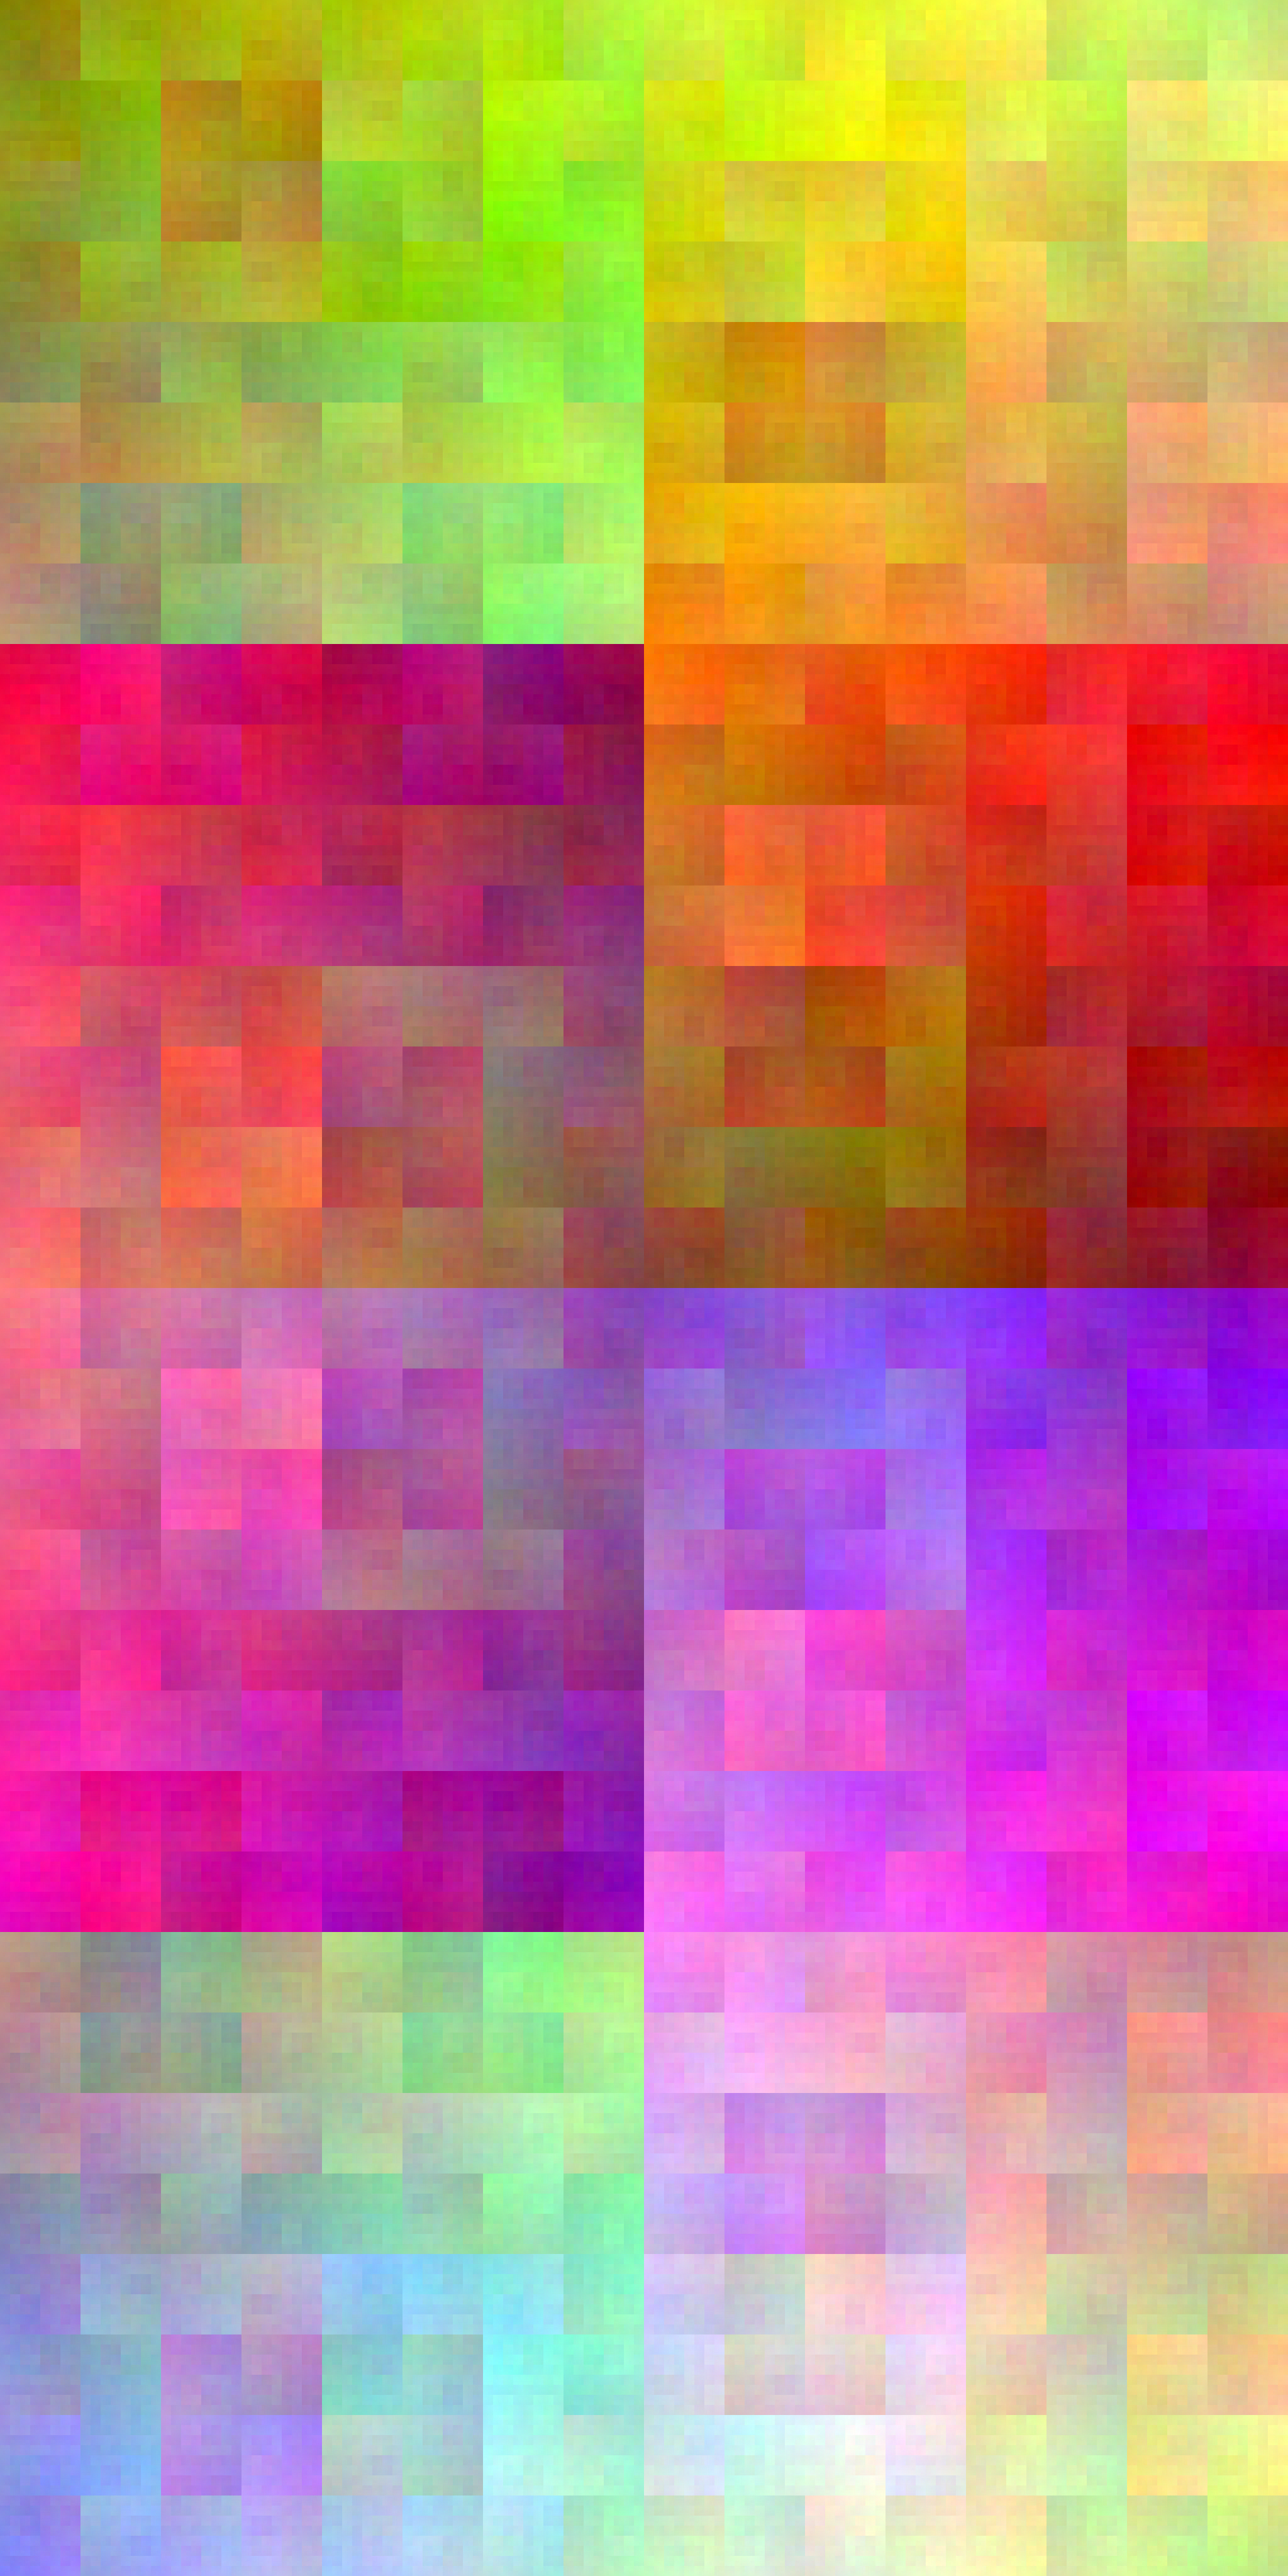
\includegraphics[width=\paperwidth]{\chapdir/pics/hilbert.png}};
\draw[anchor=north] (midpoint)  node [fill=ocre!30!white,fill opacity=0.6,text opacity=1,inner sep=1cm]{\Huge\centering\bfseries\sffamily\parbox[c][][t]{\paperwidth}{\centering Elementary Mathematical Analysis\\[15pt]
{\Large Precalculus / Derivatives}\\[20pt]
{\huge Robert Marshall Murphy}}};
\end{tikzpicture}};
\end{tikzpicture}
\vfill
\endgroup


%----------------------------------------------------------------------------------------
%	COPYRIGHT PAGE
%----------------------------------------------------------------------------------------
\newpage
~\vfill
\thispagestyle{empty}

\noindent Copyleft \copyleft\ {\the\year}  Robert Marshall Murphy\\

\noindent \textsc{Westminster Christian Academy}\\

\noindent Licensed under the Creative Commons Attribution-NonCommercial 4.0 Unported License (the ``License''). You may not use this file except in compliance with the License. You may obtain a copy of the License at \url{http://creativecommons.org/licenses/by-nc/4.0}. Unless required by applicable law or agreed to in writing, software distributed under the License is distributed on an \textsc{``as is'' basis, without warranties or conditions of any kind}, either express or implied. See the License for the specific language governing permissions and limitations under the License.\\

\noindent Book cover by Aldo Cortesi, a portion of 
\textit{A portrait of the Hilbert curve as a young fruit salad}, which is
``a Hilbert curve traversal of the three-dimensional RGB colour space, projected onto a 
two-dimensional Hilbert curve covering the plane.\\

\noindent \LaTeX\ layout taken from \textit{BYU Textbook} by J. Peatross and M. Ware\\
\noindent \textit{First printing, July 2017} 



\frontmatter
%!TEX root =  ../main.tex

\chapterimage{pano-5.jpg}
\mychapter{Introduction}{introduction}

\section{Motivation}

This textbook exists to facilitate a class coming after Algebra II and before Calculus II.  It is meant
to be a coherent mixture of Paul A Foerster's \textit{Precalculus with Trigonometry} and his
\textit{Calculus: Concepts and Applications}.  Some students can handle moving at a much 
faster pace through Precalculus topics, and hence cover the first four chapters of \textit{Calculus}.  
A student should not be expected to 
do well on the AP exam after this class (without additional side work), because of inadequate
time spent on integrals.  

\personfeature[-2.2in]{foerster}{Paul
    Foerster}{1936-, U.S.A.}{taught mathematics at Alamo Heights 
    High School in San Antonio, Texas, from 1961 to 2011\cite{BuckleyFoerste}
    . After earning 
    a BS in chemical engineering, he served four years as an engineering 
    duty officer with the Navy's Nuclear Propulsion Program. Tutoring 
    high school students while on active duty, he found his true passion 
    --- seeing students get the ``Aha!'' reaction as they finally grasp new 
    concepts. After completing his Navy service, he went back to college 
    for a spring and a summer to get his teaching certification. His teaching 
    has been interrupted only by a year's leave of absence to earn a master's 
    degree in mathematics through an academic year institute awarded by 
    the National Science Foundation.}
    

Once a school is over a certain size, and the pool of students to draw from is sufficient, there may
be the critical mass needed to create an accelerated class for those who can proceed quickly through 
the skills and understanding needed to appreciate calculus.  While it may be possible in such
situations to promote kids sooner, it may also make sense to wait until their junior year, in which case
an analysis class is a possible solution.  Students are introduced to categories of 
functions, with an eye towards their uses in calculus, at the same time.  At best, a student would proceed
from this class to a Calculus II class, which would move quickly through derivatives and 
spend most of its time on integrals.  At worst, if a student (barely) made it through this class, they would
no doubt do well in an AB class, and have time to go back and master derivatives.


\section{Prerequisites}
  
Students are expected to have performed well in a strong Algebra II class, and retain excellent
arithmetic, graphing, and factoring skills.  This textbook contains an extensive set of appendices 
, some of which should
be assigned as summer work.  We recommend thorough consultation with the sophomore teacher
to see which areas need more work and require additional assignments.  It is burdensome, but we
also highly recommend making assignments due at regular intervals throughout the summer, perhaps
via electronic submission.
American summer breaks are too long, and students forget a great
deal over three months.  Because of the exploratory nature of assignments in the appendix, it is
possible to assign exercises which were not covered at all in Algebra II, with little or no instruction.

% used to have calculator here

This textbook contains many calculator lessons for the Texas Instrument 83 or 84 (hereafter \textbf{TI-8*}).
This antiquated device may be taken into the AP, ACT, and SAT exams, and hence 
should be thoroughly mastered by a student who wishes to maximize his or her tools.  Other
devices may be used, but are unwise, since the TI-8* is the most powerful tool allowed in the 
standardized tests.



\section{Worldview}

It is highly remarkable how many  mathematics textbooks begin without  
prolegomena of any kind.  Such an oversight belies all of mathematical work, which seeks 
to establish foundations and ascertain unassailable truths.  We will attempt to counter this trend
in the shortest space.

\personfeature[-1.0in]{Immanuel_Kant_001}{Immanuel
    Kant}{1724-1804, Prussian}{was a German philosopher, and is
    is considered a central figure in philosophy. He argued that the 
    human mind creates the structure of experience, that reason 
    is the source of morality, and that the world as it is ``in-itself'' is 
    independent of our concepts of it. He is sometimes credited with 
    being the greatest Modernist philosopher, and yet laying the
    ground from which Post-Modernism sprung.
    \href{https://en.wikipedia.org/wiki/Immanuel_Kant}{(Wikipedia)}}

The universe in which we find ourselves doing mathematics is a 
reasonable and orderly one.  The Ancient Greek distinction between `cosmos' 
and `chaos', or the Biblical separation of the watery abyss from the peaceable land are
metaphors in recognition of this fact.  The ethical and personal disorder which we bring to the world
does not belie its inherent predictability.  
God has not absconded from his creation, but has
chosen to mediate himself, leaving us with the ability and responsibility to discover
what is hidden in the material world (Proverbs 25:2).  It is only by suppressing this truth that one could
pronounce as Einstein did that, ``The most incomprehensible thing about the universe 
is that it is comprehensible.''\footnote{Albert Einstein, \emph{Journal of the Franklin Institute}, Physics and Reality, p221,1936.}.
Only by \textit{a priori} rejecting the Judeo-Christian worldview -- that a reasonable and rational God
has made human beings in his image, and that we are therefore capable of thinking his thoughts
after him, and making true statements about the world -- can we understand comments such 
as Kant's ``[W]ir auch, gleich als ob es ein glücklicher unsre Absicht begünstigender Zufall wäre, 
erfreuet (eigentlich eines Bedürfnisses entledigt) werden, wenn wir eine solche systematische 
Einheit unter bloß empirischen Gesetzen antreffen.''\footnote{
[We rejoice when, just as if it were a lucky chance favoring 
our aim, we do find such systematic unity among merely empirical laws.] \textit{Critique of Judgment}, 1790.}
Rationality in human discourse and orderliness in the natural world are not things
which need to be proven but which must be presupposed for any proofs to be made.

Mathematics is not a construct of the human mind.  It is entirely foreseeable and 
understandable that advances in number theory later yield results in cryptography,
or that esoteric processes such as analytic continuation, produce useful dividends in
quantum physics, long after they are discovered.  Mathematics is the representation
and conceptualization of the invisible, created world.  Human beings are the representation
of the maximally personal God in the impersonal media of time, energy, and matter. 
`Number' and other mathematical features are part of human language:
doing math is part of what it means to be human.  It is part of \emph{what} we are,
it is good, and it is imperative --- an integral component of our purpose.

\section{Method}

\personfeature[-0.6in]{Albert_Einstein_(Nobel)}{Albert
    Einstein}{1879-1955, German}{was a theoretical physicist, and
    TIME's person of the century.  He is considered to be one of the
    smartest men of the the modern era for his revolutionary Special
    Theory of Relativity, and again for General Relativity.  He stated
    on numerous occasions that he could not ``imagine some will or 
    goal outside the human sphere'' and hence it is a happy
    coincidence that mathematics and science are so
    mutually affirming.
    \href{https://en.wikipedia.org/wiki/Albert_Einstein}{(Wikipedia)}}

Human beings are not mere containers of information.  Teaching is not plugging-in
a download wire from the side of the teacher's head into that of the students.  Most
things of value are \emph{caught}, not taught.  It is expected that a teacher will show the 
lessons in this book to their students in the context of a safe, loving relationship, which
is of necessity personal, and therefore costly.  Eventually, students should feel safe to
fail in this class, because only failing produces change and ultimately learning.  Success
only confirms us in our biases.
Of course, no one likes to fail, so every class must balance a three-legged stool: structure, 
support, and challenge.

If at all possible, teachers should present the material from a given lesson from a different
perspective than it is shown herein.  This gives the student the opportunity to read the book,
should they wish for another angle on the matter.  If students know how to learn, they should
be able to do the \textbf{problems} on their own, and spend class time presenting their 
thoughts to others, or working through the \textbf{exercises} and discussing the book.  
The first section of each chapter (after the first) is somewhat informal and self-explanatory, 
and should be assigned as homework after the previous test without instruction.

Math assignments should never consist of 10 easy exercises, rotely completing the task defined
in the lesson, followed by 10 harder exercises, followed by 5 word-problems.  Problem sets
should be a journey, that is, should possess a narrative arc.  Class periods should do the same.
Students must learn to ask themselves questions, a process they should see modeled in the
teacher.
``What did we just learn?  How can I summarize it in my own words?  How do I think it
will be applied?  How does it relate to what I already know?  When was this encountered
for the first time, and in what context (history)? How can it help me 
understand more of the myriad things above my level?  How do I solve difficult problems
involving this principle? What might this become in my life and in the lives of my
neighbors?  How can I communicate this to others?  What are some common misunderstandings
people have when encountering this material?''

Finally, while we do have a volume of material we wish students to learn and retain,
it is irresponsible to allow students to think they have ``mastered'' mathematics.  Anyone
with a Masters degree in any field has been dislodged from his or her notion that one
can know \emph{everything} about anything.  When the Ph.Ds tell us they do not know all
there is to know about even a sliver of their discipline, we did not believe them ... at first.
But slowly, over years of paper-writing and drilling down into the subject, we see even they
can not know how much there is to know about one topic within their discipline! This is
only discouraging if we are delusional enough to think that our achievement is the 
\textit{summum bonum}, the highest good.
We can indeed learn true things and asymptotically approach full understanding, but no
amateur should be so deluded as to think they know all there is to know about some
field within mathematics.  Hence, many lessons should include a taste of just how much
more there is to know, including problems that cannot be fully solved.


\section{To the Student}
\marginfig[-0in]{TI-84_Plus}{The TI-84+.\label{fig:TU84}}

This is both a textbook and a workbook.  ``Math is not a spectator sport'', and that means
you do not understand something until you've tried it.  Don't shortchange yourself by reading a
section before you've attempted the problems.  If you want to read ahead, that's fine, but
try the assignment before the reading.  Even if you don't get it all, consider it part of the reading.
Unless specifically asked to, we recommend you do not Google the answers.
Do you want to understand
the world?  Do you know that you are in a protected space, a safe time to explore and 
make mistakes, a time that you will not be afforded later?  Take the time to learn as you go, 
and you will learn how to learn, a lesson you can use for the rest of your existence.  If you get
desperate, cultivate relationships with human beings who can ask you questions that
allow you to discover the answer yourself, not be spoon-fed.

Always look out for \textbf{bold} words, in the problems, in the readings, and in the exercises.
Copy them down into your notes and try to define them for yourself, before you look in the
glossary or online. We
encourage you to take notes in the Cornell style.  This simply involves you drawing a large,
left-of-center capital `I' over your entire note page before you begin, taking notes as usual
in the right section, adding subject and paragraph headings on the left, and making
succinct summaries at the bottom of the page, perhaps a few before the test.  Headings,
your name, and the date should go across the top.
There are many videos on the internet about `Cornell Notes'.

\section{To the Teacher}

All the material in the prerequisites needs to be covered, ideally before the year begins.  
Chapters 1-12 and 14 are the minimum.  Chapter 16 and 18-20 exist for the teacher's sake,
to allow variety over the years.  Ideally, that next class would use Foerster's excellent
\textit{Calculus} textbook, taking a month to review chapters 1-4, and then moving 
on to the rest of the book, perhaps augmented the material with some lessons from
multivariable calculus and/or differential equations.

In a perfect world, every capable student would take Calculus II and Statistics
before graduating high school, but we don't live in that world.  Time permitting, discrete
topics should be broached, especially with students who will not take Stats.  The other discrete topics
are here as aides for those who have never seen them before.  
Appendices B, C, and D exist for the teachers who love those topics and wish
to expand or vary the chapters from year to year.  There is always one student who can tell
they are not getting the whole story and will not let it rest!

Classes should consist of a brief introduction or grabber, the ``problem'' set, a succinct lesson, and then
discussion as much as possible.  Ideally, every class period will end with students summarizing what
they have learned and speculating about what it could become, or what they will do next.  Homework
should consist of careful note-taking and selected exercises.


\newpage
%----------------------------------------------------------------------------------------
%	TABLE OF CONTENTS
%----------------------------------------------------------------------------------------


\pagestyle{empty}%
\newgeometry{left=2cm,right=2cm,bottom=2cm,top=2cm}%
\chapterimage{\chapdir/pics/city-night-explosion-firework}
\setcounter{tocdepth}{2}
\tableofcontents
\restoregeometry%

\cleardoublepage

\chapterimage{\chapdir/pics/paul-gilmore-192469}
\addcontentsline{toc}{chapter}{\textcolor{ocre}{Index}}
\label{ch:index}
\printindex

\cleardoublepage 
\pagestyle{fancy}% 				Print headers again


%----------------------------------------------------------------------------------------
%	Main Sections
%----------------------------------------------------------------------------------------
\mainmatter%
\part{Linear Transformations}\label{pt:linear}%
%\renewcommand{\chapdir}{ch01}%!TEX root =  ../main.tex

\mychapters{Functions}{functions}{\chapdir/pics/Mountain-type_Woodland_Caribou}


Functions are the central objects of investigation in many subdivision of mathematics today, and
are very effective means of representing real-life phenomena. For example, in any given year, 
there is one population of
deer in a certain forest.  Would it make sense for a forest ranger to answer you two numbers when
you ask how many \textit{Rangifer tarandus} (caribou) exist in a given range, at a certain time?


\begin{figure}[h]
\centering
\begin{tikzpicture}
    \begin{axis}%
    [
        %grid=major,     
        xmin=0,
        xmax=12,
        axis x line=bottom,
        ytick={0,10,...,100},
        ymax=110
       % axis y line=middle,
    ]
        \addplot%
        [
            blue,%
            mark=none,
            samples=100,
            domain=0:12,
        ]
        (x,{1+100/(1+exp(-x+5))});
    \end{axis}
\end{tikzpicture}
\caption{Population of caribou over time}
\end{figure}

How do we model phenomena in the world?  Is it reasonable to expect
caribou population to follow a curve such as the above figure?  How can we 
extract information from a graph like this?  If actual measurements diverge some
from the expectation established by the curve, are they \emph{wrong}?  Are functions
better tools than relations?  What else could there be?

\newpage
\chapterminitoc

This chapter is entitled functions.  You have been studying functions for several years now,
and should be familiar with function notation.  It is also possible to present functions 
graphically, or in a table.  Lastly, we may write or speak a verbal description of a function,
but this requires technical jargon, with which you are just starting to become familiar.

Hopefully, your time in algebra classes until now has helped you achieve a basic familiarity
with certain elementary or parent functions.  You will need to recognize them in each
of the four ways.  These prototypical versions can be moved or stretched as needed.  They
can also be mirrored or reflected.  This should naturally lead to the observation that some
graphs are unchanged under certain types of reflection.

Lastly, we will introduce the rich and vast field of taking numerical data and generating
an algebraic equation, called regression.  


%								1 - 1
\newpage
\invisiblesection{Representations}
\marginlessinput{\chapdir/0101p}
\newpage
%!TEX root =  ../main.tex

\subsection{Numerical, Graphical, Algebraic, and Verbal}


\objective{Use functions defined numerically, graphically, algebraically, or verbally.}



A \gls{function} is a relation that uniquely associates members of one \gls{set} 
with members of another set.  
More simply, a function connects members of a \gls{domain} to members of a \gls{range}, 
with the proviso that each element in the domain maps onto only one element in the range.  
When graphing a function, it is customary to plot the \emph{input} or \gls{independent variable} 
on the $x$-axis (going left to right), and the \emph{output} or \gls{dependent variable} on 
the $y$-axis (going down to up).  The independent variable is so-called because it may 
be arbitrarily chosen from within the domain.  The dependent 
variable is then forced to be a particular value (by the function).

\subsubsection{Numerically}
Typically, information is gathered about the physical world as \gls{discrete} numbers, 
occurring at fixed points. Such information may be represented as in  table ~\ref{tab:Numerically}.

\columntable[-0.75in]{1.6in}{
  \begin{tabular}{ lr }
  \hline
  \textbf{x} (months since) & \textbf{y} (100's of \$)\\
  \hline
  0 & 1200.00 \\
  1 & 840.00 \\
  10 & 1680.24 \\
  16 & 2072.98 \\
  23 & 2264.72 \\
  36 & 4303.93 \\
  48 & 6770.53 \\
  \hline
  \end{tabular}
   }{Monthly income represented numerically\label{tab:Numerically}}
    
    
\subsubsection{Graphical}
A helpful way to visualize relationships between input and output 
sets is a \gls{graph} of the function.  Similar techniques
include diagrams (see Figure for an example) and maps (see Figure for an example).  
``Mapping diagrams'' blur the line between numerical and graphical data 
(see Figure ~\ref{fig:graphically} for an example).

\begin{figure}[h]
\centering
\begin{tikzpicture}
\begin{axis}[samples=500,domain=0:48,restrict y to domain =0:8500]
\addplot[very thick,orange ]plot (\x, {1000*(pow(1.04,\x))+200*cos((\x r)*3.1415)});
\end{axis}
\end{tikzpicture}
\caption[Graph]{Monthly Income  - Graphically\label{fig:graphically}}
\end{figure}


\subsubsection{Algebraically}
Typically, graphs come from humans or machines plotting many, 
many points derived from an \gls{algebraic} formula.
Algebra is a powerful tool for describing natural phenomena, 
but it cannot do everything.  Important numbers
--- such as \gls{pi} or $e$ --- cannot be defined via algebraic techniques.  
Worse, many confuse manipulation of the symbols with actually mathematics.
However, the symbols are very concise, as you might see in Tab.~\ref{tab:algebra}.

\columntable[-0.75in]{0.3in}{
\begin{center}
$y=1000\cdot1.04^x+200\cos(\pi x)$.
\end{center}}
{Monthly Income - Algebraically\label{tab:algebra}}



\subsubsection{Verbally}
Ordinary language serves us well most of the time, with an average level of 
precision and an average level of
emotional content.  Sometimes, however, what we wish to convey is more 
meaningful and deep than
regular wording can describe.  Conversely, we might wish to exclude a whole 
host of meanings, and narrowly
zoom in on precise terminology, in order to avoid error to the fullest extent possible
(see Fig.~\ref{fig:lol}).

\marginfig[-0in]{\chapdir/pics/levelsoflanguage}{Levels of language\label{fig:lol}}

Most of us encounter poetic language\index{language} in the form of songs, since ours is an 
age sadly bereft of
poetry, something that was not true a century ago or more.  Another common 
phenomenon is to meet 
technical language when it is not expected or welcome, such as when we read the 
instruction manual for new
hardware or legal documents.  However, such documents are typically not aiming at 
easy comprehension, but
precision.  Like most jargon, they tend to use mostly ordinary words in extraordinary 
ways, similar but opposite
to poetry.

Mathematics is no difference.  This textbook is a formal setting, and as such, 
it uses technical language, carefully
choosing each word according the conventions and definitions ``in house''.  
As you cross the threshold into the
beginning stages of advanced mathematics, you must cultivate the skill of 
using this ``jargon'', something you 
do not ordinarily do.  It may help your comprehension to paraphrase 
what you are learning into the ``vernacular'',
but you should not consider a topic concluded until you are able to 
re-articulate the mater in mathematical terminology.
For example, the equation above might be described as in Fig.~\ref{fig:verbally}.

\begin{figure}
\emph{The income ($y$) may be modeled by the number of months since 
inception ($x$) as a sinusoid with an amplitude of 200, a period of 2, and a
midline of an exponential growth rate of 4\% beginning at \$1,000.}
\caption{Monthly Income - Verbally\label{fig:verbally}}
\end{figure}

\subsubsection{Mathematical Models}
Functions that can be used to make predictions and 
interpretations of real-world phenomena are called \textbf{mathematical
models}.
It is important to be clear which variable is being used as input 
and which is output, so that a meaningful
relationship between independent and dependent variables 
can be ascertained.  In the model of income above,
time does not depend upon money, but rather money upon time.  
The domain of the function is the initial time
index of zero until four years later, so in months $0\le x \le 48$.  
The income varies from as low as \$840 but
generally goes up from there, so the range is $y\ge840$.

\begin{example}
	\exProblem
There are only so many hours in a day.  If you decide to stay up \emph{all} night studying, 
you will surely get
a bad grade on the test tomorrow, due to sleep deprivation.  
Sketch a reasonable graph showing hours spent studying the day before
a test and the grade you will get on said test.  Give the domain and range of the function.

	\exSolution
One cannot possibly get less than zero hours of sleep, and presumedly around 
12 or so hours of sleep is
long enough to have slept through the exam and angered one's parents!  
Test scores are typically measured in percents, ranging from 0 to 100.

\marginfig[-1.8in]{\chapdir/pics/sleep.png}{Possible graph of sleep vs. grade}
\end{example}

~\vfill
\newpage
\subsection{Exercises}
\marginlesspdf{\chapdir/0101xA.pdf}
\marginlesspdf{\chapdir/0101xB.pdf}
\marginlesspdf{\chapdir/0101xC.pdf}



%								1 -2
\newpage
\invisiblesection{Types}
\subsection{Pick x, Find y}
\marginlesspdf{ch01/0102p.pdf}
\newpage
%!TEX root =  ../main.tex


\objective{Connect names of types of equations with graphs.}


We have said that a function is a relation of inputs to outputs, with no more than one output per input.  
We have learned that functions can be defined graphically, algebraically, numerical, or verbally.
A function that is defined by an algebra equation usually has a descriptive name.
In this section, we will look at several groupings of various functions, some of which you should
be very familiar with, and some of which may be new.


You might be used to seeing a  \gls{graph} of certain equations, written algebraically with $y$ in terms
of $x$, like $y=x$.  These have then been graphed on the Cartesian plane, as a continuous curve,
with each point corresponding to an ordered pair, $(x,y)$.  Leonhard Euler created much of the notation
we use today, including \emph{function notation}: $y=f(x)$.

\marginfig[-0in]{\chapdir/pics/Linear_Function_Graph.png}{Linear functions.\label{fig:LinearFunction}}
\subsubsection{Linear}
One of the most obvious things to see is a straight line.  
Humans create straight lines seemingly more often
than anything else.  Hence, lines can feel unnatural or reassuring.  
What are some of the properties of lines?
How might two lines be the same?  How might they differ?  

\marginfig[-0in]{\chapdir/pics/AndraGrad-4}{A quadratic function is a polynomial of degree two.}
Lines could have the same slope, and therefore never run into each other.  
They would only be distinguished by their
heights.  For convenience, we measure the height of a \gls{linear} function 
in Analytic Geometry by its starting value, its $y$ when $x$ 
equals zero.  Conversely, these starting locations might be the same and 
slope might be different.  You have learned \index{linear!intercept form}
to distinguish these two different variables as $m$ and $b$, as in $y=mx+b$, and we shall see
that it is expedient to distinguish them \textbf{constant} functions, $y=k$.
\index{constant!function}

\subsubsection{Quadratic}
Many things in our world operate over two dimensions, such as gravity.  
Hence, Newton find that the force
of two objects upon each other is proportional to the \emph{square} of their distance.  
Squares graphed make a
\textbf{parabola}, a word reference the path of a falling or thrown object.  
Algebraically, we can see all such shapes\index{quadratic!standard form}
have an equation of the form $y=ax^2+bx+c$, which is called \gls{quadratic}.  
You should already know a great deal about quadratics from previous classes.

\paragraph{Power}
As more dimension interact, the exponent on $x$ can become very 
complicated, and even fractional.  We can generalize\index{power function!standard form}
from $y=x$ to $y=x^2$ and $y=x^3$ to $y=a\cdot x^b$.  We shall study them in more depth
in chapter 5.

\paragraph{Polynomial}
A sum of power functions with whole number exponents is called a
\textbf{polynomial}.  Such equations are among the most well-studied
areas in mathematics.  A polynomials divided by a polynomial is called
a \textbf{rational function}.  Both are the subject of chapter 6.
\index{polynomial}\index{rational function}

\subsubsection{Exponential}
\marginfig[-0in]{\chapdir/pics/2^x_function_graph}{$2^x$ is an  exponential function}
Quantities that experience the same percentage growth or decay 
year over year look similar in the algebra: $x$ is in
the exponent, and hence such an equation is called an \gls{exponential} function.  The general form
is $y=a\cdot b^x$.  \index{exponential function!standard form}
The ``opposite''\footnote{There are \emph{many} things 
which could be called `opposite'
in mathematics, so this is not technical language.  We will define `inverses' of functions in 4.4.} of such a 
function is a called a \gls{logarithm}, and we will follow the TI-8* for now and use the generic equation
$y=a+b\ln{x}$.  \index{logarithmic function}

\subsubsection{Periodic}
Many phenomena is nature reoccur the same way at regular intervals.  Such functions are said to be 
\textbf{periodic}.
We will  study `simple harmonic motion', which comes from components of motion in circles, in section III,
Trigonometric Functions.  For now\footnote{Later, we
will factor the ``inside'', but this first kind is the sort produced by your grapher.}, use the general equation $y=a\cdot\sin(bx+c)+d$.\index{sine function}

\inlinefig{\chapdir/pics/Periodic_function_illustration.png}{\label{fig:periodic}A periodic function is so called because it repeats at a given interval, called the period (P).}

\newpage
\subsection{Exercises}
in Kuta
~\vfill


%								1 - 3
\newpage
\invisiblesection{Translations and Dilations}
\subsection{Multiplying and Adding Functions}
\marginlesspdf{ch01/0103pA.pdf}
%\newpage
\marginlesspdf{ch01/0103pB.pdf}
\newpage
%!TEX root =  ../main.tex
\subsection{Inside vs. Outside}


\objective{Produce and decipher translations and dilations of functions.}


\subsubsection{``Outside'' Operations}
How would you triple the output of a function?  How would you add four the output of a function?
Because function notation means ``perform the operation of the function upon the input'', we must
write the operators we described \emph{to the right} of the function operation, written $f(x) \cdot 3$
and $f(x) + 4$ respectively.  Normally, multiplicative operators are written on the left, without
an intervening symbol.  Because addition is commutative, it may be written on the left as well.

\paragraph{Addition}
\marginfig[-1in]{\chapdir/pics/verticaltranslation}{Vertical translation is outside addition.}
What is the graphical effect of the algebraic operation, $f(x) + 4$?  Let us build up a visual picture
numerically at first.

\emph{adding moves it up, negatives move it down.  Multiplication by $>1$ makes it taller.
$(0,1)$ makes it shorter.  All relative to the x-axis.}

\begin{example}{Outside Transformations}
	\exProblem
$r(x)=\sqrt[3]{x}$ and $s(x)=\frac{1}{2}r(x)+3$.  In what ways does the graph of
$s(x)$ differ from $r(x)$?

	\exSolution
up 3, half as tall
\end{example}
\index{transformation!translation}

\paragraph{Multiplication}
Multiplication also behave as one might expect, effecting $y$ in a directly-proportional way.
For example, regardless of what $f(x)$ is (excepting 0), then the graph of $3\cdot{}f(x)$
with be three times taller, a vertical dilation of 3.

\subsubsection{``Inside'' Operations}
Things done ``inside'' are done \emph{before} the function operates on the domain.  This means
graphically they will effect $x$.  However, their effect is quite curious, typically being the 
\emph{opposite} of what one might expect.

For example, consider the quadratic function $f(x)=x^2$, and a transformation of it, $g(x)=f(x+4)$.
We can see that the +4 is on the ``inside'', and we know that 4 is added to members of the domain
before they are plugged in to the function.  This means -4 will become 0 before it is squared.
Another way to say this that what used to be outputted at $x=0$ will now be outputted at $x=-4$.

This opposite effect also applies to dilations.  When we multiply the inside of a function by 2, it does
not produce a graph twice as wide, but \emph{half}.

\begin{example}{Inside Transformation}
	\exProblem
Consider the continuous function $f(x)$ given by the graph (looks like a radical sign).
Describe and graph the continuous $g(x)$, when $g(x)=f(2x-2)$.  What would be a more
informative way to write $g(x)$ in terms of $f(x)$?

	\exSolution
It's half as wide and left 1.  $f(2(x-1))$ would be more transparent.
\end{example}
\index{transformation!dilation}

In summary, $f(x) + d$ will shift the graph $d$ units to the right.  $f(x+c)$ will shift the graph
$c$ units to the left.  $a\cdot{}f(x)$ will make the graph $a$ times taller.  $f(b\cdot{}x)$ will
make the graph $b$ times skinnier.

~\vfill

\newpage
\subsection{Exercises}
in Kuta
~\vfill


%								1 - 4
\newpage
\invisiblesection{Reflections and Symmetries}%
\marginlessinput{ch01/0104p}
\newpage
%!TEX root =  ../main.tex
\subsection{Reflection}


\objective{Produce reflections of functions and describe their symmetry.}


As you know, multiplying numbers by $-1$ produces the additive opposite: negative values
become positive and positives become negative.  Zero is unaffected, being neither positive
nor negative.  The same principle applies to functions.  What would it look like to ``flip'' all
$x$ values?  $y$ values?

\paragraph{``Outside''}
$-f(x)$ is a reflection over the $x$-axis, leaving $x$'s untouched, and making $y$'s opposite.

We can obtain both the original and reflection across the $x$-axis by writing $\pm f(x)$.  Why
is that not a function?

\paragraph{``Inside''}
$f(-x)$ is a reflection over the $y$-axis, leaving $y$'s untouched, and making $x$'s opposite.

Does the ``opposite'' rule of inside transformations apply or not to the negative on the inside?
\index{transformation!reflection}


\subsection{Symmetry}
\paragraph{Even}\index{even functions}
\marginfig[-0in]{\chapdir/pics/Playing_card_spade_A.png}{The ace of spades (or of clubs or hearts) displays even symmetry about its center.}
Sometimes, multiplying by a negative makes no difference.  In mathematics, this can be very 
helpful to know.  Functions that are the same left-to-right and right-to-left are called \textbf{even}.
Can you guess why?  Aren't only numbers even (or odd)?



\begin{derivation}{Even Functions}
An even function has the property $f(x)=f(-x)$ for every $x$ in its domain.
\end{derivation}



Among the more basic functions are power functions.  We will study them in great depth in
chapter 5.  The names ``even'' and ``odd'' come from the similar behavior of $x^n$ when
$n$ is even or odd.

Notice that evenness has the visual appearance of putting a mirror on the $y-$axis.  Did you 
know human beings are made to find such left-right symmetry appealing?  Study the faces of
attractive people, and you will find evenness to be a rule of thumb. 



\begin{derivation}{Odd Functions}\index{odd functions}
An odd function has the propety $-f(x)=f(-x)$ for every $x$ in its domain.
\end{derivation}


\marginfig[-0in]{\chapdir/pics/English_pattern_queen_of_hearts.png}{The queen of hearts (and many other playing cards) display an odd symmetry about the center.}
You might have supposed oddness to be top-to-bottom and bottom-to-top symmetry.  Why isn't
that possible for functions?  Instead, we find that these functions are the same whether we 
proceed left from the origin, or flip the right half upside-down.


\paragraph{Rotational}\index{rotation!symmetry}
Looking at the odd power functions, it becomes clear that there are two ways to regard their
symmetry.  Either they are reflections left-right and up-down (in either order), or they are
$180^\circ$ of themselves.  Is it possible for a function to have any other angle of symmetry
with itself?

Moving on to symmetry \emph{between} functions (or relations), we see a lot of rotational
symmetry exists.  All lines of the form $y=ax$ are rotations of each other.  $f(x)=x^2+k$ and
the relation $y=\pm\sqrt{x-k}$ are $90^\circ$ rotations of each other.

Relations can be their own rotation.  Equilateral triangles with their center at the origin are 
all $120^\circ$ rotations of themselves.  In fact, every regular $n-$gon (polygon) is its
own rotation every $\frac{360}{n}^\circ$.  As we take the limit and let $n$ increase,
we approach circular symmetry, continuous rotational symmetry.

Rotation is hard to discover under normal algebra, but it very easy with a matrix.
You can read in §18.1 how the rotational matrix is 
$\begin{bmatrix} 
	\cos { \theta  }  & -\sin { \theta  }  \\ 
	\sin { \theta  }  & \cos { \theta  }  
\end{bmatrix}$.


\inlinefig{\chapdir/pics/Purple_Star}{Rotational symmetry becomes much more complicated in higher dimensions.}


\newpage
\subsection{Exercises}
in Kuta


%								1 - 5
\newpage
\invisiblesection{Regressions}
\subsection{Graphical Patterns}
\marginlesspdf{ch01/0105pA.pdf}
\newpage
\marginlesspdf{ch01/0105pB.pdf}
%!TEX root =  ../main.tex

\subsection{STATS in the TI}

\objective{Create appropriate regressions of data in a grapher.}


In order to proceed from numerical to algebraic and graphical models of
real-world situations, we need to perform \textbf{regression analysis}, a thoughtful
process of establishing the strength and kind of relationship between two
variables.  The entirety of Chapter 13 is about regression.
For now, we simply seek to make equations from sets of ordered pairs.
\index{regression}

\index{TI-8*!data entry}
Your TI-8* has \emph{some} capacity as a spreadsheet.  You may entered tabular data, 
graph, and analyze the results on this little computer!  Most things you will need start by
pressing the \Touche[style=function,principal={stat},raise=-5pt] button.
This information is stored in lists, like \texttt{L$_1$}, \texttt{L$_2$}, \texttt{L$_3$}, etc.  
These names are not letters found via the \Touche[style=alpha]
button, but are whole characters.  They can be accessed via \Touche[style=second]
\Touche[style=number, principal=1,second=L1], \Touche[style=second] 
\Touche[style=number, principal=2,second=L2], etc.  The most normal way to proceed is to put $x$ 
data in \texttt{L$_1$} and $y$'s in \texttt{L$_2$}.


Next, in order to make data you've entered visible, one must turn on a \texttt{STAT PLOT}.
This is done via \Touche[style=second] 
\Touche[style=graph,principal={y=},position = 0.9,second={stat plot},raise=-7pt].
Here you will see three different \texttt{STAT PLOT}s you can turn on or off.  Press
\Touche[style=enter,principal=enter,raise=-5pt] to select one, and then again to turn it on.
Be sure to turn \texttt{STAT PLOT}s off when you're not using them, so as not to obfuscate
other graphs.

\reminder{\lefthand}{
It is always faster to press the number than the \Touche[style=arrows, raise=-0.15cm,scalearrows=0.2]
and scroll through the menu:

\Ecran[width=4,height=3]{{\renewcommand\tabcolsep{-7pt}
\begin{tabular}{ll}
\Menu[size=10,select=true]{ZOOM} & \Menu[colourbox={ForestGreen!15}, size=10]{MEMORY} \\[-8pt]
\multicolumn{2}{l}{\Menu[colourbox={ForestGreen!15}, size=9, text={ZBox}]{1 :}} \\[-8pt]
\multicolumn{2}{l}{\Menu[colourbox={ForestGreen!15}, size=9, text={Zoom In}]{2 :}} \\[-8pt]
\multicolumn{2}{l}{\Menu[colourbox={ForestGreen!15}, size=9, text={Zoom Out}]{3 :}} \\[-8pt]
\multicolumn{2}{l}{\Menu[colourbox={ForestGreen!15}, size=9, text={ZDecimal}]{4 :}} \\[-8pt]
\multicolumn{2}{l}{\Menu[colourbox={ForestGreen!15}, size=9, text={ZSquare}]{5 :}} \\[-8pt]
\multicolumn{2}{l}{\Menu[select=true, size=9, text={ZStandard}]{6 :}} \\[-8pt]
\multicolumn{2}{l}{\Menu[colourbox={ForestGreen!15}, size=9, text={ZTrig}]{7 $\downarrow$}} 
\end{tabular}
}/
}
}

\subsubsection{Windows}\index{TI-8*!window}
One of the trickier things to manage on the TI-8* is the \texttt{WINDOW}.  The Cartesian plane is 
a big place, and finding your place in it can be harder still.  Having a grasp
on concepts like \gls{domain} and \gls{range} is once again worth it's weight in gold.


First of all, the TI-8* does try to help you out by offering several automatic options, which 
may or may not be  useful.  The most commonly used is 
\Touche[style=graph,principal=zoom,position=0.9,raise=-5pt]
\Touche[style=number, principal=6,raise=-5pt]: \texttt{ZStandard}.  This is the common window, 
$-10\le x\le 10$ and $-10\le y\le 10$, with tick-marks every unit.  When in doubt, start here.

If, however, the data is given to you, make the \texttt{Xmin} the smallest element in the domain,
and \texttt{Xmax} the biggest (press WINDOW).  Similarly, the range should dictate your \texttt{Ymin} and 
\texttt{Ymax}.  For truly useful graphs, determine the breadth of both the domain and range, 
by subtracting the smallest element from the biggest.  Divide these by 20 and you will get
the \texttt{Xscl} and \texttt{Yscl} respectively (the little tick marks).

Of course, the procedure outlined in the last paragraph will not work for most function definitions,
since they will go on forever, often in both domain and range.  This means you just have to know
what are the salient features of a given kind of graph, and how to bring them into view.  For example,
a quadratic function's most important point the vertex, the place where it changes from increasing
to decreasing or visa versa.  Most of the time, this is involves a process of guess-and-check,
combined with every-honing instincts.

\subsubsection{Table}\index{TI-8*!table}
\Touche[style=second] \Touche[style=graph,principal={graph},position=0.9,fontsize=7pt,raise=-5pt] is
the very helpful \texttt{TABLE} of data.  This is especially useful at comparing multiple functions on 
the same inputs.  The default to start at $x=1$ and increment by one from there on up.
To customize the table, you must press \Touche[style=second] 
\Touche[style=graph,principal=window,position=0.9,fontsize=7pt,second=tblset,raise=-10pt].  
You can either make the table 
automatically increment through the domain, starting where you wish and skipping by the
same amount every time (\texttt{AUTO}), or you can manually enter values for the input (
\texttt{Ask}).


\paragraph{Linear Regression}
In you are given only two points and told to make a line through them both, then the problem is 
very easy system of two equations, and can be immediately solved via the RREF of a 2x3 matrix.
However, most scientific and real-life data is ``fuzzy'', and no line can go through all the data points.
In such situations, it is best to enter all the data and let the machines find the ``line of best fit''.  In 
simple cases, it is simply a matter of constructing the line where half the data is below and half is 
above.  But as data multiplies, this becomes harder and harder.\index{regression!linear}

\begin{example}{Linear Regression}
\exProblem
Find the line of best fit for the data in this table.

\begin{tabular}{c|c}
   \textbf{x} & \textbf{y} \\ \hline 
   1 & 1 \\
   2 & 2 \\
   3 & 1.3 \\
   4 & 3.75 \\
   5 & 2.25 \\
\end{tabular}

\exSolution
Using a TI-8*, press \Touche[style=function,principal=stat], \texttt{EDIT}, and enter the $x$ data in 
$L_1$ and the $y$ data in $L_2$.  If
there is already data clogging up these lists, move up to their names at the top of the window
and press \Touche[style=function,principal=clear]  \Touche[style=enter,principal=enter,raise=-5pt].  Assuming
the appropriate STATPLOT is on, press \Touche[style=graph,principal={zoom},position=0.9,fontsize=7pt]
\Touche[style=number,principal=9] and inspect the graph.  It is not a simple linear graph, where
any line passing through any two of the points is perfect, so we proceed with the calculator's regression
program.

Pressing \Touche[style=function,principal=stat], moving over to \texttt{CALC}, we scroll down to 
\texttt{LINREG(AX+B)}.  Depending upon your version,
you may need to type $L_1, L_2, Y_1$ or select all these setting for a menu.  ($Y_1$ is located under
\Touche[style=function,principal={vars},raise=-5pt], \texttt{Y-VARS}, \texttt{FUNCTION}, etc. and should be 
entered under \texttt{Store EQ}.) Press \Touche[style=enter,principal=enter] or \texttt{CALCULATE}
and the answer of $y=.425x+.785$ appears, as well as the coefficient of determination, $r^2$.  
\reminder{\lefthand}{If your
calculator doesn't show you $r^2$, you might need to press \Touche[style=second] 
\Touche[style=number,principal=0,second=catalog], scroll down to \texttt{DiagnosticOn}
and turn it on.} We will learn about $r$ and $r^2$ in §13.3, but for now it is enough to say it is helpful
measure of how closely the equation ``hugs'' the data.

Finally, press \Touche[style=graph,principal=graph,position=0.9,fontsize=7pt,raise=-5pt] to see the equation 
against the data.
\end{example}

\paragraph{Quadratic Regression}\index{regression!quadratic}
When the data rise and falls (or falls and rises), it is possible that a quadratic equation would be a better fit.
Visualize the data and then consider running QuadReg and generating an equation of the form $ax^2+bx+c$.
Perfect data can be solved simply with a 3x4 matrix.

\paragraph{Exponential and Logarithmic Regression}\index{regression!exponential}
ExpReg and LnReg are great tools, if you know how to choose between them.

\includegraphics[scale=0.8]{\chapdir/pics/expln.png}\index{regression!logarithmic}

Exponential functions have a horizontal asymptote at $y=0$ if un-translated.  Logarithmic functions
has a vertical asymptote at $x=0$ if un-translated.  Most practical situations, it is always possible to tell if
there is a limiting $x$ or $y$ value.  If there are multiple asymptotes, it is probably a power function.

\paragraph{Sinusoidal Regression}\index{regression!sinusoidal}
While we have not formally introduced period functions yet, it is relatively easy to run a SinReg in the calculator
and get an equation from data.  The only additional questions you must answer are the number of iterations ---
how many times should the calculator pour over the data (the max is 16, which you should use for all ``fuzzy''
data) --- and the \textbf{period} --- the distance from peak to peak, or trough to trough.  For now, the period will
always be given to you.

\newpage
%!TEX root =  ../main.tex
\columntable[0.1in]{2.4in}{
\begin{center}
\begin{tabular}{c|c}
	\textbf{Year} & \textbf{\$} \\ \hline
	1990 & 10.19\\
	1991 & 10.50\\
	1992 & 10.75\\
	1993 & 11.03\\
	1994 & 11.32\\
	1995 & 11.64\\
	1996 & 12.03\\
	1997 & 12.49\\
	1998 & 13.00\\
	1999 & 13.47\\
	2000 & 14.00\\
	2001 & 14.95\\
	2002 & 14.95\\
	2003 & 15.35\\
\end{tabular}
\end{center}
}{Hourly earning\label{tab:hourly}}

\columntable[0.8in]{1.3in}{
\begin{center}
\begin{tabular}{c|c}
  \textbf{mph} & \textbf{ft} \\ \hline
  20 & 23.9 \\
  30 & 33.7\\
  40 & 40.0\\
  50 & 41.7\\
  60 & 46.8\\
  70 & 48.9\\
  80 & 49.0\\
\end{tabular}
\end{center}
}{Breaking distance\label{tab:break}}

\columntable[0.6in]{2.0in}{
\begin{center}
\begin{tabular}{c|c|c|c}
	\textbf{Month} & \textbf{NY} & \textbf{DC} & \textbf{TX} \\ \hline
	Jan. & 32 & 43 & 62\\
	Feb. & 34 & 47 & 65 \\
	Mar. & 43 & 56 & 72 \\
	Apr. & 57 & 67 & 80 \\
	May & 69 & 75 & 87 \\
	Jun. & 78 & 84 & 92 \\
	Jul. & 82 & 88 & 96 \\
	Aug. & 80 & 87 & 97 \\
	Sep. & 72 & 80 & 91 \\
	Oct. & 60 & 68 & 82\\
	Nov. & 48 & 58 & 71 \\
	Dec. & 36 & 47 & 63 \\
\end{tabular}
\end{center}
}{Temperatures\label{tab:temps}}

\renewcommand{\columnseprule}{1.5pt}
\begin{multicols*}{2}
\rule[0.5\baselineskip]{0.4\textwidth}{1pt}
\noindent%
\ExSection\label{sec:0105x}
\begin{exercises}{sec:0105x}
\prob[0105Quad1] Find a quadratic model for the given data.\footnote{CA textbook 13-16}
\subprob \{(1,-1), (2,1), (4,8), (5,14), (6,25)\}
\subprob \{(1.5,-2.2), (2.2,-4.8), (3,4), (-11,2), (5.1,-20.6)\}

\prob[0105Quad2]
\subprob \{(-2,-5), (-1,0), (0,1), (1,4), (2,4)\}
\subprob \{(1.5,-2.2), (2.2,-4.8), (3.4), (-11,2), (5.1,-20.6)\}

\prob[0105Arch] The data below shows the length of the humerus and the total wingspan, in
centimeterss, of several pterosaurs (extinct flying reptiles). \footnote{CA textbook 17}
\subprob Compute a linear regression for these data
\subprob On the basis of this model, which is the projected wingspan of a 
\textit{Quetzalcoatlus northropi}, which is estimated to have has a humerus of 54 cm?  
Round to the nearest centimeter.



\prob[0105ModelDay] For a particular day of the year $t$, the number of 
daylight hours in New Orleans can be approximated by 
$$
d(t)=1.792\sin\left(\dfrac{2\pi(t-80)}{365}\right) + 12.145
$$
where $t$ is an integer and $t=1$ corresponds to January 1.\\ According to $d$, 
how many days per year will New Orleans have at least 10.75 hours of daylight?



\prob[0105Hourly] The average hourly earnings of U.S. production
workers for the 1990's are shown in Table~\ref{tab:hourly}.\footnote{Demana Precalc p163}


\subprob Produce a scatter plot of the hourly earnings ($y$) as a function
of the years since 1990 ($x$).
\subprob Run the linear regression and store it in $Y_1$.
\subprob Record the $r^2$ value.  Does it suggest that this model is appropriate?
\subprob Run the quadratic regression and store it in $Y_2$.
\subprob Record the $r^2$ value.  Does it suggest that this model is appropriate?
\subprob Find the difference between the two models' predictions for the average hourly earnings in 2010.
\subprob Write a four sentence paragraph describing why it can be risky to extrapolate from a mathematical
model, citing your work here in technical language.


\prob[0105traffic]
A traffic safety institute measured the breaking
distance, in feet, of a car traveling at certain speeds in miles per hour.
The data from one of those tests are seen in Table~\ref{tab:break}.\footnote{CA 28}
\subprob Find the quadratic regression equation for these data points.
\subprob Using the regression model, predict the breaking distance
when a car is traveling at 65 mph?  Round to the nearest tenth
of a foot.


\prob[0105LM1]
\begin{tikzpicture}[remember picture,overlay]
\coordinate (here) at (3,-3);
\draw (current page.west |- here) node[right]{
\begin{tabular}{c|c}
  \textbf{Time} & \textbf{Altitude ($^{\circ}$}) \\ \hline
  7:00 & 9.6 \\
  8:00 & 22.0 \\
  9:00 & 34.1 \\
  10:00 & 45.2\\
  11:00 & 54.3\\
  12:00 & 59.5\\
  13:00 & 58.7\\
  14:00 & 52.2\\
  15:00 & 42.4\\
  16:00 & 30.9\\
  17:00 & 18.7\\
  18:00 & 6.2\\
\end{tabular}
\par\\
\textbf{Table:Sun}\label{tab:sun}
};
\end{tikzpicture}%to prevent adding extra space before text
Use a $2 \times 3$ matrix and the TI-8* command RREF to solve for the
$A$ and $B$ of a line in intercept form (i.e. $Ax+B=y$) that passes
through the following two points (answer in fractions):
\subprob (-3,4) and (7,8)
\subprob (2,0) and (4,0)
\subprob $(\frac{2}{3},\frac{1}{6})$ and ($4\frac{1}{3},7\frac{5}{6})$
\subprob (-2.3,-4.7) and (-6.9,-6.5)

\prob[0105LM2]
\subprob (1,-2) and (-3,3)
\subprob (-4,-4) and (4,4)
\subprob $(\frac{5}{3},-3)$ and $(-\frac{1}{3},5)$
\subprob (2.14,-3.2) and (-0.11,1.64)


\prob[0105high] Table~\ref{tab:temps} shows the highest daily temperature  
averaged over the month for the cities of 
Syracuse, NY; Washington DC; and Austin, TX.  Create sinusoidal regressions for each 12-month 
pattern and predict in which month the three cities will have the same daily high. 
\footnote{from the website \url{http://mathbits.com/ MathBits/ TISection/ Statistics2/sinusoidal.html}}



\prob[0105sun] Table~\ref{tab:sun} below shows the altitude for the
sun in Dallas, Texas, at selected times during September 15, 2013. \footnote{CA 97}
\subprob Find the sine regression function that models 
the altitude in degrees of the sun as a function of the
time of day.  Use 24.017 hours (the time from sunrise
on September 15 to sunrise September 16) for the period.
\subprob Use your regression equation to estimate the altitude
of the sun on the 15th at 9:30 a.m.  Round to the nearest
tenth of a degree.


\prob[0105newton] A $190^\circ F$ cup of coffee is placed on a desk in a $72^\circ F$ room.
Newton's Law of Cooling say that the temperature at time $x$ obeys the
following equation: $T(x) = (T_0-T_a)b^x+T_0$, where $T_0$ is the
initial temperature, $T_a$ is the ambient temperature around, and $b$ is 
a constant that depends upon the substance being cooled.  The following
table shows the recorded temperature at one minute intervals of the coffee
\footnote{Demana}
\begin{tabular}{c|c}
	\textbf{Time} & \textbf{Temp.} \\ \hline
	1 & 184.3 \\
	2 & 178.5 \\
	3 & 173.5 \\
	4 & 168.6 \\
	5 & 164.0 \\
	6 & 159.2 \\
	7 & 155.1 \\
	8 & 151.8\\
	9 & 147.0\\
	10 & 143.7\\
\end{tabular}
\begin{tabular}{c|c}
	\textbf{Time} & \textbf{Temp.} \\ \hline
	11 & 140.0\\
	12 & 136.1 \\
	13 & 133.5 \\
	14 & 130.5\\
	15 & 127.9 \\
	16 & 125.0\\
	17 & 122.8\\
	18 & 119.9\\
	19 & 117.2\\
	20 & 115.2\\
\end{tabular}


\subprob Make a scatter plot of the data, with time in $L_1$ and temperature
in $L_2$.
\subprob Under STAT-EDIT, move onto $L_3$ and enter that it equals $L_2-72$.  Run the exponential regression, being sure to use $L_1$ and $L_3$, and store it in $Y_1$.  Record the $r^2$ value.
\subprob Suffix a ``+72'' to $Y_1$.  Record your equation.  
\subprob How well does your function fit the data, both numerically and visually?

   
\end{exercises}
\end{multicols*}






%								1 - 6
\newpage
\section{Review}
%!TEX root =  ../main.tex
\subsection{Chapter Review}
This chapter was about functions, and how they model so much of reality.  Functions can be
described numerically (tables), algebraically (formula), graphically (Cartesian plane curves), or
verbally (technical language).  Some functions we have seen before or will see in this course
are linear, quadratic, exponential, power, rational, logarithmic, and periodic.
You need to have memorized the simplest form of each type of equation (Tab.~\ref{tab:generalequations}).

\columntable[-0.75in]{2.8in}{
    \textbf{Linear:}\\  $y=m\cdot{}b$

    \medskip

    \textbf{Inversely Proportional:}\\
    $y=\frac{k}{x}$

    \medskip

    \textbf{Power:}\\
    $y=a\cdot{}x^b$

    \medskip

    \textbf{Quadratic:}\\
    $y=ax^2+bx+c$

    \medskip

    \textbf{Exponential:}\\
    $y=a\cdot{}b^x$

    \medskip

    \textbf{Logarithmic:}\\
    $y=a+b\ln{x}$

    \medskip

    \textbf{Periodic:}\\
    $y=a\cdot\sin(b(x-c))+d$
    }{General equations\label{tab:generalequations}}


You should review the graphs of each of these.  In fact, you should attempt to engage all
these forms in all four ways.

Functions are written in function notation, which looks annoyingly like multiplication.
Functions can have operations done on them, as numbers do, only they have two place where
operators may be applied: inside (before) and outside (afterwards).  Outside effects the output
(y) and is reasonable.  Inside effects x and is contrarian!  Adding translates (moves) the graph.
Multiplying stretches (dilates) the graph.  Negatives `flip' the graph.  Graphs that are the same when flipped
left/right are called even, like even powers of x.  Graphs that look the same when they are
flipped left/right \emph{and} up/down are called odd, like odd powers of x.  The calculator can help us turn
numerical data into function notation via it's many regression functions.

Some questions you should be prepared to address are:
What are functions?  What are some of the basic types of functions?  What are the four ways
we describe functions in this chapter?  How do we move between the various descriptions?
What happens to $f(x)$ as we vary four constants, like this: $a\cdot{}f(b(x+c))+d$?
What are some of the differences between our models and reality?  What have previous classes
shown you to be the nature of the mathematic task?  What is technical (vs ordinary or poetic)
language?  What role does technical language play in your life, now and presumedly in the future?


\begin{figure}
\begin{centering}
\begin{tikzpicture}[->,>=stealth',shorten >=1pt,auto,node distance=5cm, semithick]
  \tikzstyle{every state}=[fill=red,draw=none,text=white]

  \node[state,minimum size=2cm] (A)                    {Graph};
  \node[state,minimum size=2cm]         (B) [above right of=A] {Data};
  \node[state,minimum size=2cm]         (D) [above left of=B] {Equation};
  \node[state,minimum size=2cm]         (C) [above left of=A] {Verbal};

  \path (A) edge [bend right=5]              node[below,sloped] {``read''} (B)
            edge [bend right=5] node[above,sloped] {``describe''} (C)
            edge [bend right=5,dotted]  node[below,sloped]  {``find''} (D)
            edge [loop below]	node {``change''} (A)
           (B) edge[bend right=5] node [above,sloped] {``plot''} (A)
           edge [loop right] node {``convert''} (B)
           edge [bend right=5]  node[above,sloped] {``regress''} (D)
           edge [bend right=20] node [above,sloped] {``characterize''} (C)
           (C) edge[bend right=5] node[below,sloped] {``sketch''} (A)
           edge [bend right=5] node[below,sloped] {``build''} (D)
           edge [bend right=20] node[below,sloped] {``estimate''} (B)
           edge [loop left] node {``paraphrase''} (C)
           (D) edge [loop above] node {``algebra''} (D)
           edge [bend right=5] node[below, sloped] {``tabulate''} (B)
           edge [bend right=5] node[above,sloped] {``explain''} (C)
           edge [bend right=5,dotted] node[below,sloped] {``graph''} (A);
\end{tikzpicture}
\caption{Some possible words to describe moving among the four representations\label{fig:16relationships}}
\end{centering}
\end{figure}

Figure~\ref{fig:16relationships} is not the final word(s) on relating the four representations,
but it is supposed to get you thinking.  We often manipulate symbols and change one
equation type into another, but we can do the same with graphs.  Paper does not
allow it, but couldn't we build an object that changes color over time, in order to
represent a function?  Data could be changed from absolute $x$ and $y$ to
``number of steps since last'' and ``percent change''.  Try to come up with a simple 
model of a natural phenomenon and see how many relationships you can
fulfill.

\subsection{Chapter Test}
\noindent\makebox[\textwidth]{\includegraphics[width=\paperwidth]{ch01/01testA.pdf}}
\newpage
\noindent\makebox[\textwidth]{\includegraphics[width=\paperwidth]{ch01/01testB.pdf}}
 
 
 
%
%\renewcommand{\chapdir}{ch02}%!TEX root =  ../main.tex

\mychapters{Limits}{limits}{\chapdir/pics/EDMcrowd}

%%%%%%%%%%%%%%%%%%%%%%%%%%%%%%%%%%%%%%%%%%%%%%%

Limits are a way of expressing what a function's output approaches as the input gets
closer and closer to a given value.  In this section, we will use limits to describe the 
location of ``holes'' in graphs, continuous functions, asymptotes and sided-limits, 
the difference quotient and derivatives.

Sound engineers use advanced functions to design waveforms that would not occur in nature.
The distinctive sound of much of today's electronic music comes from computer approximating
what infinite sums of sounds waves would sound like.  Are there actual infinities in the physical
universe?  If something cannot exist without human creativity, what does that mean about its
place in the world, its ``rightness'' or ``wrongness''?

\marginfig[-1in]{\chapdir/pics/Sawtooth_Fourier_Analysis.JPG}{Much of today's EDM music makes use of sounds only possible through approximating infinite sums of waves.}

How should we treat our responses to questions where we cannot verify our answers?
Should we only interpolate, or is extrapolation also valid?  Is it reasonable to assume
things continue after the manner we have observed when they are unobserved, or even
unobservable?  Is anything in our universe able to be modeled with only one function across
all of its domain? What good is it to instantaneous change, when change -- by definition --
happens over time?



\newpage
\chapterminitoc

%									2 - 1
\newpage
\invisiblesection{Removable}
\marginlessinput{\chapdir/0201p}
\newpage
%!TEX root =  ../main.tex

\subsection{First Discontinuities}

\objective{Find informal limits at holes and non-holes.}

In this section, we will explore the informal definition of a \textbf{limit}.  Have you ever had anyone
sneer at you over a lost opportunity and say, ``Should of, would of, could of''?  (It probably
sounded like ``shoulda, woulda, coulda''.)  The idea is that everyone can see a hypothetical 
in hindsight, though that does not avail you anything now.  Hypotheticals are situations describing
what was likely, or intended, or desired.  In mathematics, we often encounter functions
which appear \textit{as though} there is an expected value, only to have that spot not
even be part of the domain.

Limits are like the hypothetical situation of math.  Suppose your friend bought a ticket for a vacation,
and said they wanted to get away.  Then you didn't see this friend for a long time, and then you asked
them, ``Did you ever go on vacation?  Where were you going to go?'  You know they 
were in some sense headed somewhere, but from your perspective, it has yet to be determined if
he or she actual went and where your friend was even headed.  Notice how your second question
doesn't even depend on whether they went anywhere or not: it is about a hypothetical.  

Many functions give an indeterminate answer at certain gaps in their domain.  It is obvious
where they were ``headed'', but direct evaluation at that value in the independent variable is
not helpful.



\begin{derivation}{Indeterminate Form}
\index{indeterminate form}
For a given function $f(x)$, if $f(c)=\frac{0}{0}$, then the point $c$ represent a gap in the domain.
\end{derivation}


\subsection{Algebra Techniques}
From the perspective of algebra, there are four techniques for constructing 
precise replacements for many functions, replacements which are everywhere else the same,
but lack the particular ``hole''.

\subsubsection{Cancelling}
Consider the function $f(x) = \frac{x^2-4}{x-2}$.    Enter it in your calculator and try \Touche[style=function,principal={ZOOM},]
\Touche[style=number, principal=6].  How can it be just a line?  Why isn't it more complicated than that?  
Well, it is.  Try plugging in 2.  That is, what is $f(2)$?  $\frac{2^2-4}{2-2} = \frac{0}{0}$.


\begin{derivation}{Factor Removal}
When $f(c)=\frac{0}{0}$ and the removal of a common factor in the numerator and denominator yields a real number $d$,
then $(c,d)$ represents the location of a hole in $f(x)$.
\end{derivation}


Returning to our equation, $x^2-4$ in the numerator factors by the 
Difference of Squares to $(x-2)(x+2)$.  This is means
we can write $f(x)=\frac{(x-2)(x+2)}{x-2}$.  It is \emph{not} true that 
$\frac{(x-2)(x+2)} = x+2$: they differ in their domains.
However, $x+2$ is an \textbf{analytic continuation} of $\frac{x^2-4}{x-2}$, 
meaning is is everywhere the same as the
original but has an \textit{even larger} domain.  We may use $x+2$ to answer the q
uestion what $f(x)$ would output
at $x=2$, were it to exist there.

\subsubsection{Expanding}
Some functions obscure the factor that could be cancelled with further arithmetic.  For example, it is not obvious
what $g(x)=\frac{(x+3)^3-27}{x}$ will be at $x=0$\footnote{If you are especially keen, you might notice that this is
factorable as the difference of cubes in the numerator, but we will pretend no one saw that!}.  Sometimes a small
piece of arithmetic allows us to proceed as in the previous section.  in this case $(x+3)^3=x^3+9x^2+27x+27$.


\begin{align*}
\frac{(x^3+9x^2+27x+27)-27}{x} &=\\
\frac{x(x^2+9x+27)}{x} & \approx x^2+9x+27\\
& \rightarrow (0)^2+9(0)+27 \\
&\rightarrow 27\\
\end{align*}


\subsubsection{Complex Fractions}
\emph{Not to be confused with fractions involving complex numbers!}

Besides simple arithmetic, complex fractions can obfuscate the cancelling 
needed to simplify the presence
of a hole.  $\cfrac{2-x}{\frac{1}{x}-\frac{1}{2}}$ is indeterminate at $x=2$.  
However, if we simplify this fraction until it has a simple (non-fraction) numerator and 
denominator, the indeterminate form will evaporate.


\begin{align*}
\cfrac{2-x}{\frac{2}{2}\cdot\frac{1}{x}-\frac{1}{2}\cdot\frac{x}{x}} &= \cfrac{2-x}{\frac{2-x}{2x}} \\
&\approx \cfrac{2x(2-x)}{2-x} \\
&\approx 2x\\
&\rightarrow 2(2) = 4
\end{align*}



\begin{derivation}{Additional Factor}
When $f(c)=\frac{0}{0}$ and the multiplication by a common factor in the numerator and denominator yields a real number $d$,
then $(c,d)$ represents the location of a hole in $f(x)$.
\end{derivation}



\subsubsection{Conjugates}
What to multiply by can be difficult to decipher.  It often appears as though we might wish to square individual terms 
in the numerator or denominator.  For instance, the function $h(x) = \cfrac{\sqrt{x+1}-1}{x}$ is $\frac{0}{0}$ at $x=0$.
Clearly, we might wish to square only the upper-left corner of the fraction, in order to remove the square root.  The
secret is to recognize the numerator is of the form $a-b$, where $a=\sqrt{x+1}$ and $b=1$.  Any binomial multiplied
by it's conjugate yields the difference of squares (i.e. $(a+b)(a-b)=a^2-b^2$).  In this case, we must multiply top and
bottom by $\sqrt{x+1}+1$.


\begin{align*}
\cfrac{\sqrt{x+1}-1}{x} \cdot \cfrac{\sqrt{x+1}+1}{\sqrt{x+1}+1} &\approx \cfrac{(x+1)-1}{x(\sqrt{x+1}+1)}\\
&\approx \cfrac{1}{\sqrt{x+1}+1}\\
&\rightarrow \cfrac{1}{\sqrt{0+1}+1} = \frac{1}{2}
\end{align*}

\subsubsection{Direct Substitution}
Some time, there might seem to be a hole, but none exists.  In that case, we can simply plug
the input into the equation and get a result.

\inlinefig{\chapdir/pics/Continuidad_de_funciones_02.png}{Removable discontinuities are typically hole in the graph, places where there is no value to the function, but the expected value is straightforward to calculate.}


\newpage
\begin{defproblem}{0201:RemovableA}
\begin{onlyproblem}
\begin{exercise}[Removable Discontinues]
Find the limit of the given function at the given value.
This may require you to create a version of the given function that will 
allow you to plug in the given value.
The result should typically be a fraction.
\begin{enumerate}[itemsep=4pt,parsep=4pt]
\item $\dfrac{x^2+x-6}{x-2}$ at 2
\item $\dfrac{\sqrt{x+2}-3}{x-7}$ at 7
\item $\dfrac{(5+x)^2-25}{x}$ at -5
\item $\dfrac{x^3-6x+2}{x^2+2x-3}$ at 3
\item $\cfrac{\frac{1}{3+x} - \frac{1}{3}}{x}$ at 0
\item $\dfrac{1}{x\sqrt{1+x}}-\dfrac{1}{x}$ at 0
\end{enumerate}
\end{exercise}
\end{onlyproblem}
\begin{onlysolution}
\begin{enumerate}
\item 5
\item $\frac{1}{6}$
\item 5
\item $\frac{11}{12}$
\item $-\frac{1}{9}$
\item $-\frac{1}{2}$
\end{enumerate}
\end{onlysolution}
\end{defproblem}

\begin{defproblem}{0201:RemovableB}
\begin{onlyproblem}
\begin{exercise}[Removable Discontinues]
Find the limit of the given function at the given value.
This may require you to create a version of the given function that will 
allow you to plug in the given value.
The result should typically be a fraction.
\begin{enumerate}[itemsep=4pt,parsep=4pt]
\item $\dfrac{(x-1)^3+1}{x}$ at 0
\item $-\dfrac{2x^2+3x}{2x+3}$ at $-\frac{3}{2}$
\item $\cfrac{x}{\frac{1}{x-2}+\frac{1}{2}}$ at 2
\item $\dfrac{x^3-1}{x^3+5x^2-6x}$ at 1
\item $\dfrac{\sqrt{x^2+9}-5}{x+4}$ at -4
\item $\dfrac{\sqrt{x+\frac{29}{2}}-4}{x-\frac{3}{2}}$ at $\frac{3}{2}$
\end{enumerate}
\end{exercise}
\end{onlyproblem}
\begin{onlysolution}
\begin{enumerate}
\item 3
\item $\frac{3}{2}$
\item 0
\item $\frac{3}{7}$
\item $-\frac{4}{5}$
\item $\frac{1}{8}$
\end{enumerate}
\end{onlysolution}
\end{defproblem}
\endinput

~\vfill



%									2 - 2
%\newpage
\invisiblesection{Continuous}
\subsection{Definition of Limits}
\noindent\makebox[\textwidth]{\includegraphics[width=\paperwidth]{\chapdir/0202p.pdf}}
\newpage
%!TEX root =  ../main.tex

\subsection{Epsilon-Delta}

\objective{Use the definition to evaluate limits.}


In the last section, you experiment with finding the values that \emph{would have}
occurred in a series of functions, if there had not been a \textbf{discontinuity} at a given
point.  The value that the function approaches is called a \textbf{limit}.  Because all the
examples to date have been \textbf{removable discontinuities}, it has simply been a matter
of algebra manipulation to produce a \emph{nearly} identical version of the function, but
simply one without the hole.

In the beginning, it was sufficient to define limits as casually as we have done, which is why
2.1 is laid out the way it is.  Later, mathematicians named Cauchy and Weierstrauss created
much more rigorous definitions to meet demand.  Let us built up such rigor.
\marginfig[-1in]{\chapdir/pics/tricky}{The function appears to be a decreasing exponential ... or does it?}

\index{TI-8*!zoom box}
Here is a negative example: $f(x)=\dfrac{|x-3|\cdot1.2^x}{(x-3)\cdot12^x}+2$.  Enter the 
function as $Y_1$ and begin with ZOOM-STANDARD.  You should have a decreasing
exponential function, with a horizontal asymptote at $y=2$.  Now you should become
suspicious.  What did the $x-3$ terms produce?  Is there something going on at $x=3$,
when both terms are 0 and the entire function is $\frac{0}{0}$?  If you consult the
TABLE, you will see there is an ERROR at 3.  Let us investigate.

Practice using the ZOOM-BOX feature, drawing new windows around (3,2) until the 
discontinuity becomes clear.  Here is our window and graph:

insert figure Xmin=2.999 Xmax=3.001 Xscl=5E-4 Ymin=1.9985 Ymax=2.0015 


How can we avoid being fooled like this?  What does it mean to say ``the limit as
$f(x)$ approaches $c$ is $L$''?

\marginfig[-1in]{\chapdir/pics/epsilondelta.png}{Whenever a point $x$ is within $\delta$ units of $c$, $f(x)$ is within $\epsilon$ units of $L$ \cite{epsilondelta}.}



\begin{derivation}{Definition of a Limit}\index{Limit!definition}
$$\lim_{x\rightarrow c} f(x)=L$$


The limit as $x$ approaches $c$ of $f(x)$ is $L$, if and only if
for any $\epsilon>0$ no matter how small, there is a $\delta>0$ such that
$x$ is with $\delta$ units of $c$ but $x\ne c$, that $f(x)$ is with $\epsilon$ units of $L$.
\end{derivation}



In less compact terms, this means for \emph{any} radius $\delta$ around $c$, there is exists
a radius $\epsilon$ around $L$ that $f(x)$ stays with in.  This definition, developed by
Cauchy, is the successor to Leibniz's idea of ``infinitesimals''\footnote{
See \cite{Alexander12}.}.


\subsubsection{Continuity}
It would certainly save a lot of time if we could classify functions by whether they will
ever fail to have a limit or not.  Smooth functions, where every minuscule change in the
input results in a minuscule change in the output are called \textbf{continuous}.  A function
$f(x)$ is continuous at point $a$, if and only if:\index{continuity}
\begin{enumerate}
\item $\displaystyle \lim_{x\rightarrow a} f(x)$ exists,
\item $f(a)$ exist, and
\item $\displaystyle \lim_{x\rightarrow a} f(x) = f(a)$.
\end{enumerate}
A function that is continuous at every point in its domain is said to be a \textbf{continuous
function}.  Continuous functions whose domain is all Real numbers are said to be ``continuous
over the Reals'' or ``continuous for Reals''.


\begin{example}{Discontinuous}
	\exProblem
Is the function $f(x)=\frac{1}{x}$ continuous for Reals?

	\exSolution
No.  In fact, there is \emph{no} $\epsilon$ we could pick that the
output would stay within for any $\delta$ around 0.  The asymptote at $x=0$ shows that the
graph increases \emph{without limit}.


\marginfig[-1.5in]{\chapdir/pics/Function-1_x.png}{Function $y=\frac{1}{x}$\cite{function1x}.}
\end{example}


\begin{example}{Testing the Definition}
	\exProblem
Show that
$$
\lim_{x\rightarrow 1} (5x-3)=2
$$
	\exSolution
According the definition of a limit, we set $c=1$, $f(x)=5x-3$ and let
$L=2$.  To show that $\displaystyle \lim_{x\rightarrow 1}(5x-3)=2$, we need to show that for
any number $\epsilon>0$, there exists a number $\delta>0$ such that for all $x$,

$$
0<|x-1|<\delta \quad \Rightarrow \quad |(5x-3)-2|<\epsilon 
$$

(The symbol $\Rightarrow$ is read ``implies''.)  If we can transform our second equation to 
contain the middle term of the first, we have succeeded:

\marginfig[-1in]{\chapdir/pics/epsilonover5}{$\epsilon-\delta$ around (1,2)}
\begin{align*}
|(5x-3)-2| & < \epsilon \\
|5x-5| & <\epsilon \\
5|x-1| & <\epsilon \\
|x-1| & < \epsilon \div 5\\
\end{align*}
The last line tells us that the original $\epsilon$-inequality will hold is we choose
$\delta < \epsilon \div 5$.


\end{example}
~\vfill
\newpage
\subsection{Exercises}
Made as a Word doc.
~\vfill


%									2 - 3
%\newpage
\invisiblesection{Piecewise}
\subsection{Mind the Gap}
\noindent\makebox[\textwidth]{\includegraphics[width=\paperwidth]{\chapdir/0203p.pdf}}
\newpage
%!TEX root =  ../main.tex

\subsection{Definition}

\objective{Interpret piece-wise functions and their limits}


In human observations, there is almost nothing which follows one equation for the 
entirety of its domain.  The only constant in the universe is change!  For example, 
population of the world, the stock market, or even one stock might generally follow one
equation for a significant stretch of time, but not forever.  So it is that most functions are 
defined in pieces, and are therefore called piece-wise functions.

For example, the absolute value function which you have been using for some time now is
actually a piecewise function.\index{Absolute Value!piece-wise}

We should formally define the nomenclature of a ``sided'' limit:

\begin{derivation}{Right-sided limit}\index{limit!right-sided}
``The limit as $x$ approaches $c$ from the right is $L$'' is true if and only if for every $\epsilon > 0$, there exists a $\delta > 0$ such that
$|f(x)-L|<\epsilon$ whenever $0<x-c<\delta$.

$$\lim_{x \to c^+}f(x) = L$$
\end{derivation}


\begin{derivation}{Left-sided limit}\index{limit!left-sided}
Similarly, ``The limit as $x$ approaches $c$ from the left is $L$'' is true if and only if for every $\epsilon > 0$, there exists a $\delta > 0$ such that
$|f(x)-L|<\epsilon$ whenever $0<c-x<\delta$.

$$\lim_{x \to c^-}f(x) = L$$
\end{derivation}


\personfeature[-3in]{\chapdir/pics/George_Boole_color}{George
    Boole}{1815-1864, French}{was an English mathematician
    who said, ``No general method for the solution of questions 
    in the theory of probabilities can be established which does 
    not explicitly recognise, not only the special numerical bases 
    of the science, but also those universal laws of thought which 
    are the basis of all reasoning, and which, whatever they 
    may be as to their essence, are at least mathematical as to their form.''
    \href{https://en.wikipedia.org/wiki/George_Boole}{(Wikipedia)}}

\subsubsection{Boolean Variables}\index{booleans}
Perhaps surprisingly, your TI-8* can graph piece-wise functions.  We will start with a simple
piecewise-function :

$$
f(x)=
\begin{cases}
x, x<1\\
x^2,x\ge 1
\end{cases}
$$

\index{TI-8*!piece-wise}


If we wanted to graph the sections separately, we could make $Y_1=(X^2)/(X\ge{}1)$ and
$Y_2=(X)/(X<1)$.  (The equality and inequality signs are under 2ND-MATH --- TEST.)  This will 
allow you to make the different sections different colors or different shading, but that might be
what you want.  To graph everything in $Y_1$, use $(X^2)*(X\ge{}1)+(X)*(X<1)$.



\subsection{Other Discontinuities}
\reminder{\lefthand}{The different TI-8* behave differently around holes.  Newer calculators will attempt to make a hole apparent, while older models do not show it.

Only the new models draw points visibly, but even then they are very small.  We recommend
against even trying to represent them in the TI-8*.}


All together, there are five kinds of discontinuities.  We are only responsible to rigorously prove
instanes of the first two and the last:

\subsubsection{Removable}
Here the limit exist.  The graph has a hole in it, which may or may not be defined as a point somewhere unexpected.
\subsubsection{Jump}
The limits does not exist.  The graph is not continuous, but ``leaps'' from one output to another without passing in between, at one or more points.
\subsubsection{Infinite} 
The limit may or may not exist.  The function itself goes up and/or down without limit.  The most common example is a vertical asymptote.
\subsubsection{Oscillating} 
The limit does not exist.  The graph varies between outputs in way that never resolves.
\subsubsection{Domain} 
The limits does not exist because on one side, the function ceases to exist.



%\newpage
\subsection{Exercises}
\noindent\makebox[\textwidth]{\includegraphics[width=\paperwidth]{\chapdir/0203xA.pdf}}
\newpage
\noindent\makebox[\textwidth]{\includegraphics[width=\paperwidth]{\chapdir/0203xB.pdf}}
\noindent\makebox[\textwidth]{\includegraphics[width=\paperwidth]{\chapdir/0203xC.pdf}}




%									2 - 4
\invisiblesection{Infinite}
\subsection{Are We There Yet?}
\noindent\makebox[\textwidth]{\includegraphics[width=\paperwidth]{\chapdir/0204p.pdf}}
%!TEX root =  ../main.tex

\subsection{At Infinities}

\objective{Determine when a limit does and does not exist, or is infinite.}

Because limits are asking questions that need not have simple number inputs and
need not have simple number outputs, we can evaluate limits involving infinities.
``Infinity'' simply means ``without end''.  Asking what a function approaches as
$x$ approaches infinity, graphically means ``what value is the output tending
towards as the input grows without bound?''.  Negative infinity is a term describing
the leftward trend of function.


\begin{derivation}{Limit at Infinity}
For $f(x)$ a real function, the limit of $f$ as $x$ approaches infinity is L, 
means that for all  $\varepsilon >0$, there exists $c$ such 
that $|f(x) - L| < \varepsilon \text{whenever} x > c$. \footnote{$\forall \varepsilon > 
0 \; \exists c \; \forall x > c :\; |f(x) - L| < \varepsilon$}

$$\lim _{x\to \infty }f(x)=L$$

\end{derivation}


The same applies at negative infinity:


\begin{derivation}{Limit at Negative Infinity}\index{limit!at infinities}
For $f(x)$ a real function, the limit of $f$ as $x$ approaches negative infinity is L, 
means that for all $\varepsilon >0$ there exists $c$ such that 
$ |f(x) - L| < \varepsilon \text{whenever} x < c$.  \footnote{$\forall \varepsilon > 
0 \; \exists c \; \forall x < c :\; |f(x) - L| < \varepsilon$}


$$ \lim_{x \to -\infty}f(x) = L$$

\end{derivation}


\begin{example}
	\exProblem
Evaluate $\displaystyle \lim_{x \to -\infty}2^x$
	\exSolution
We can observe the graph or compute numerically that $2^x$ is getting closer
and closer to 0 as we move leftward.  We can get arbitrarily close to 0 by picking
whatever large, negative exponent we wish.  Hence, the answer is 0
\end{example}




\subsection{Infinite Forms}
Not only can we ``plug in'' infinities in limits problems, but we can also get
$\pm\infty$ as an answer.  Recall, however, that the left and right sided limits
must agree for the limit to exist.  Hence, we can say that the limit as $x$ 
approaches 0 of $x^{-2}$ is infinity, while the same limit taken on $\frac{1}{x}$
does not exist.


the limit of f as x approaches a is infinity, denoted

$$\lim_{x \to a} f(x) = \infty$$
means that for all $\varepsilon >0 \text{there exists}  \delta >0 \text{such that}  f(x) > \varepsilon \text{whenever}  |x - a| < \delta$.

These ideas can be combined in a natural way to produce definitions for different combinations, such as

$$f(x)=  \lim_{x \to \infty} f(x) = \infty, \lim_{x \to a^+}f(x) = -\infty$$.
For example:

$$ \lim_{x \to 0^+} \ln x = -\infty$$

%\newpage
\subsection{Exercises}
\noindent\makebox[\textwidth]{\includegraphics[width=\paperwidth]{\chapdir/0204xA.pdf}}
\newpage
\noindent\makebox[\textwidth]{\includegraphics[width=\paperwidth]{\chapdir/0204xB.pdf}}
\noindent\makebox[\textwidth]{\includegraphics[width=\paperwidth]{\chapdir/0204xC.pdf}}



%									2 - 5
\section{Change}
\subsection{Extremely Average}
Word doc
\newpage
%!TEX root =  ../main.tex

\subsection{Difference Quotient}


\objective{Explain the various forms of the difference quotient and their meaning.}


To all appearances, limits seem to be about incredibly precise --- more precise
than anything in our universe --- or unmeasurably large inputs of functions.
This would seem to offer us nothing useful about the world we actually find ourselves
in.  Such is not the case, however.

If we want to know about the rate of change of a function, we must typically ask 
``over what interval?''  We might suspect that there is a moment on the graph below
($x\approx.25$) where the average rate of change is 0.  How might we prove that?
We would have to travel some further amount in the $x$ direction, which would
produce some change in the $y$ value, because the rate of change is $\frac{\Delta y}
{\Delta x}$.

\begin{figure}
\begin{center}
\includegraphics[scale=0.6]{\chapdir/pics/dq.png}
% http://www.texample.net/tikz/examples/difference-quotient/
\caption{The difference quotient, as $\Delta x$ approaches 0\cite{tikzdq}.}
\end{center}
\end{figure}

In single-variable calculus, the difference quotient is usually the name for the expression
\begin{equation}
\lim_{h\rightarrow0}\frac {f(x+h)-f(x)}{(x+h)-x}
\end{equation}

What does this represent?  We are looking for the rate of change of the function.  We begin
by inputting $x$ (and, of course, receiving an output of $f(x)$).  We then move over a tiny 
amount and measure the change in output, over the change in input.  That tiny amount is called
$h$, and we take the limit as $h$ goes to 0.

Because we are evaluating the entire function this way, if we are able to answer the limit, 
we will receive a new function as out answer.  This function is called the \textbf{derivative} of
$f(x)$.


\begin{derivation}{Derivative}
The derivative of a function $f(x)$ may be denoted $f'(x)$.  This style of writing is
called \textbf{Lagrange's notation}, after Joseph-Louis Lagrange
\end{derivation}


\begin{figure}
\begin{center}
\includegraphics[scale=0.9]{\chapdir/pics/deriv.png}
\caption{The difference quotient produces a secant line \cite{derivativedefinition}.}
\end{center}
\end{figure}

Sometimes it is too difficult or time consuming to find the entire derivative equation.
We might want to find the derivative at one location only, typically called $c$

\begin{equation}
\lim_{x\rightarrow c}\frac{f(x)-f(c)}{x-c}
\end{equation}

These tend to be much easier to solve, as they are typically removable discontinuities
of the kind we solved in §2.1

\subsection{Theorems of Limits}
Let's us generalize the properties of limits we have seen in action this chapter:
\begin{enumerate}
\item The limit of a product is the same as a product of limits
\item The limit of a sum is the same as a sum of limits
\item The limit of a quotient is the same as a quotient of limits (but $\ne 0$)
\item The limit of a constant times a function is the same as a constant times a limit
\item the limit of a constant is a constant
\end{enumerate}

~\vfill
%\newpage
\subsection{Exercises}
\noindent\makebox[\textwidth]{\includegraphics[width=\paperwidth]{\chapdir/0205xA.pdf}}
\newpage
\noindent\makebox[\textwidth]{\includegraphics[width=\paperwidth]{\chapdir/0205xB.pdf}}


%									2 - 6
\section{Review}
\subsection{Chapter Review}
This chapter was generally new ideas, that we might describe where a function ``would've gone'',
whether it ended up with a value or not.  This idea --- called a limit --- has a formal definition with
the Greek letters $\epsilon$ and $\delta$, which correspond to the ``error'' in the $y$ values
resulting ``differences'' in the $x$/input.  Limits allowed up to define what a continuous 
function is.  We saw that a function might be composed of pieces ... and still be continuous.
There are four ways to remove discontinuities.  There are five kinds of discontinuities.
The powerful language of limits extended to describe phenomena at infinities, as well as ``values'' 
of the infinities.  Ultimately, limits were used to make possible difference quotients, the 
average rate of change of a function at an instant.

\subsection{Chapter Test} 
%\renewcommand{\chapdir}{ch03}%!TEX root =  ../main.tex

\mychapters{Parents}{parents}{\chapdir/pics/Elakala_Waterfalls_Swirling_Pool_Mossy_Rocks}

Why is most of our universe so easy to model?  
Is it valid to divide the world into dimensions,
or are those purely human constructs with no external reality?  
Is it necessary to think in more 
than one dimension at once?  More than two?  
What good is instantaneous information when 
time continues to flow and never stops anyway?

Some of the simplest functions to deal with are lines, which is why your education
up to this point as largely focuses on them.  Lines through the origin model directly
proportional variables.  Their opposite --- you recall --- are inversely proportional
variables, and produce a weird looking graph called a hyperbola.  But even hyperbolas
look like lines, if you zoom in far enough.  So do parabolas.  And roots.  Lastly,
we will see what a how velocity information can tell us about position ...
and what it can't.

\newpage
\chapterminitoc


%							3 - 1
\newpage
\invisiblesection{Linear}
%!TEX root =  ../main.tex
\renewcommand{\columnseprule}{1.5pt}
\begin{multicols*}{2}
\rule[0.4\baselineskip]{0.4\textwidth}{1pt}
\noindent
\LabSection{In Pieces}\label{sec:0301p}
\begin{exercises}{sec:0301p}
\lab{} There is a function called the \textbf{floor} function, written
$f(x)=\left\lfloor x \right\rfloor$.  In the TI-8*, it is called \texttt{int(},
found under MATH-NUM.  Graph the function under a standard 
window and sketch a copy below.  Describe what you
think the function does to the input in your own words.

\vspace{3cm}
\lab{}  In the function continuous?  If not, where not?  

\vspace{3cm}
\lab{} Select an appropriate locus and calculate the instantaneous rate of change
of the function.  Extrapolate for all Reals, and write a piecewise function
for the derivative of the floor function.

\vspace{3cm}
\lab{} Another common function from computer science is the \textbf{remainder}
function, typically called \texttt{mod} in most programming languages, or is just written with
a percent sign (\%).  It can be reproduced quite simply on the TI-8*.  For example,
$g(x)=x\%5$ can be entered as $Y_2=X-5int(X/5)$.  Sketch a graph below.
How would \emph{you} define the remainder function?  

\vspace{4cm}
\lab{} Find $g'(2)$.  The recurrent discontinuities should be obvious.  Write
a piecewise function for the derivative of the modulus function $y=x\%n$
for any $n$.

\vspace{4cm}
\lab{} A linear but periodic function is hard to define.  We will cheat and simply
linearize a periodic function: $h(x)=2\cos^{-1}(\cos(x\pi\div2))\div\pi-1$.%
%Let $Y_1=|fpart(X/2)|$. 
%Let $Y_2=remainder(iPart(|X|),2)$.  
%But only leave on $Y_3=2|Y_2(X)-Y_1(X)|$.
Sketch a graph below.

\vspace{4cm}
\lab{} Unlike the previous functions, this one has no discontinuities.  However,
there are an infinite number of places where the instantaneous rate of change
is incalculable.  Define \emph{all} the places where the difference quotient will not
work and we cannot find the derivative.

\vspace{3cm}
\lab{} What did you learn as a result of doing this exploration that you did not
know before?
\end{exercises}	
\end{multicols*}
\newpage
%!TEX root =  ../main.tex
\subsection{Properties of Lines}

\objective{Classify linear and linear-like functions, and explain relationships of slopes.}


All non-vertical lines have slope, which is defined as rise over run, $\frac{\Delta x}{\Delta y}$ 
or $m$.  The initial value
of a linear equation might not be zero, but an ordered pair of the form $(0,b)$.  The variable
$b$ is called the $y-$intercept.  All together, this is the famous $y=mx+b$ form of lines.

\marginfig[-0.1in]{ceiling_function}{The ceiling function.}
However, that formula only makes sense when the origin is within view and we might become 
concerned with the output-value when the input is 0. In calculus and other areas of mathematics, 
we are more
often simply interested in the slope and some arbitrary point, $(x_1,y_1)$.  Hence we find a majority
of time from here on out, the point-slope form of \index{linear!point-slope form}
linear equation is most helpful, $y-y_1=m(x-x_1)$,
a form which allows us to see the slope, and a (random?) point on the line very easily.
This form is nearly as easy to put in your TI-8* as your old friend slope-intercept: simply add $y_1$
to the other side, and you have a $y=$ form ready to be entered in your grapher.

\subsection{Parallel vs. Perpendicular}
If a line has slope expressed via the fraction in lowest terms $\frac{a}{b}$, 
then any other fraction that reduces to the same ratio will produce a line parallel to the first.  
Consider the sketch of how to make a line rotated $90^\circ$ clockwise or counterclockwise 
to the first.  They will have slopes of $\frac{-b}{a}$ or $\frac{b}{-a}$, which are the same
things.  In short, perpendicular lines have opposite reciprocal slope.\index{linear!parallel}
\index{linear!perpendicular}

\subsection{Linear-like}
Several functions are linear in pieces, and are used in computer programming and other
systems of functions

\subsubsection{Ceiling, Floor, and Round}
Various forms of rounding are present in computer systems and your TI-8*.  Rounding down
in all cases, rounding up in call cases, and the familiar rounding to the closest.

\marginfig[0in]{floor_function}{The floor function}
\subsubsection{Modulus}
The most used function in this respect, and the foundation of an entire species of mathematics
(called Modular Arithmetic) is the modulus function.  It can be thought of as taking two arguments,
one is what to divide by, and the other is what to divide.  The function returns the remainder.  For
example, 10 mod 3 is 1, and 49 mod 7 is 0.  Consider the graph of y=x mod 5.

\subsubsection{Rates of Change}
A constant function is one that never changes (by definition).  \index{constant!derivative}
Algebraically, that means it is
of the form $y=c$, where $c$ is some numbers.  The slope is always zero and the graph
is always a horizontal line.  A vertical line is not a function and its slope is undefined.  Every
other line has a constant rate of change, it's slope.  In calculus terminology,
it's derivative is a constant.







\newpage
\subsection{Exercises}
%\loadallproblems[0301]{problems/0301x}
%\begin{multicols}{2}
%\renewcommand{\theenumi}{\thesection.\arabic{enumi}}
%\begin{enumerate}[leftmargin=0cm,itemindent=.5cm,labelwidth=\itemindent,labelsep=0cm,align=left]
%\foreachproblem[0301]{\item\label{prob:\thisproblemlabel}\thisproblem}
%\end{enumerate}
%\end{multicols}
%\renewcommand{\theenumi}{\arabic{enumi}}





%							3 - 2
\newpage
\invisiblesection{1/x}
%!TEX root =  ../main.tex
\renewcommand{\columnseprule}{1.5pt}
\begin{multicols*}{2}
\rule[0.5\baselineskip]{0.4\textwidth}{1pt}
\noindent
\LabSection{Zoomed Straight}\label{sec:0302p}
\begin{exercises}{sec:0302p}
\lab{} Input the function $f(x)=\frac{4}{x}$ into your TI-8* and view
it under ZOOM-STANDARD.  Press \Touche[style=second]
\Touche[style=function,principal={zoom}] and FORMAT your
window to have the GRID ON.  What lattice points (i.e., where
$x$ and $y$ are both integers) does the graph pass through?

\vspace{2cm}
\lab{} What do you estimate the rate of change of the function is around 
$f(2)$? Record you guess here.

\vspace{1cm}
\lab[] Using the ZOOM-BOX feature, outline a new window from (0,0) to
approximately (4,4).  Again, draw a ZOOM-BOX, now from about  (1,1)
to (3,3).  Change your \texttt{Xscl} and \texttt{Yscl} to 0.2.  Sketch the 
resultant graph here.

\begin{center}
\begin{tikzpicture}[scale=0.5]
    \foreach \x in {0,1,2,3,4,5,6,7,8,9,10}
    \foreach \y in {0,1,2,3,4,5,6,7,8,9,10}
    {
    \draw [gray] (\x,\y) circle (0.1cm);
    }
    \draw [black, -] (-1,-1) -- (-1,11) -- (11,11) -- (11,-1) -- cycle;
  \end{tikzpicture}
\end{center}
  
\lab Manually zoom in this time, by adjusting the WINDOW so that your
$x$ and $y$ min and max are, respectively, 1.5 and 2.5.  Change both scales
to 0.1.  Press TRACE and move left and right along the graph.  What 
grid points does the equation pass through?  

\vspace{3cm}
\lab  Make your window 1.99 to 2.01 and your scale 0.002 in both directions.
You should see an almost completely straight line.  TRACE a pair of coordinate,
one just a little left and up from (2,2) and one just a little right and down.  Find
the slope of the line through them, rounding to the nearest integer.  
Record the equation in slope-intercept form,
with that slope, passing through (2,2).

\vspace{3cm}
\lab{} Moving the $y_1$ term to the other side, enter your line as another equation
on your TI-8*.  Turn off the GRID and change your scales to 1.  ZOOM-OUT
from the point (2,2) repeatedly, until you approximate ZOOM-STANDARD.
What have you drawn?

\vspace{3cm}
\lab[] Using the different quotient, work out the derivative of $f(x)=\frac{4}{x}$ below.
What is $f'(2)$?

\vspace{3cm}
\lab[] It appears that --- on a small enough scale --- inversely proportional graphs
are \textbf{locally linear}.  What other functions do you think might display 
this property?  Experiment on the calculator.  Where you right?

\vspace{4cm}
\lab[] Describe what you think the point of this problem set is, using technical vocabulary in complete
sentences.
\end{exercises}
\end{multicols*}
\newpage
%!TEX root =  ../main.tex

\subsection{Local Linearity}

\objective{Define derivatives and find numerical approximations}


When two variables grow proportionally to each other, they obey the algebraic relationship
$y=ax$.  This means when one goes up, the other goes up, and visa versa.  But many things
in nature are \emph{inversely} proportional to each.  \index{proportion!inverse}
That is, when one goes up, the other goes
\emph{down}.  This is the algebraic relationship $y=\frac{a}{x}$.

\personfeature[-1in]{\chapdir/pics/Henri-Poincare}{Jules Henri Poincar\'{e}
    }{1854-1912, French}{was a French mathematician and physicist
    who discovered many amazing facets of modern physics and non-
    traditional mathematics.  He was true polymath of his time, and
    never worked very long on a problem, relying (successfully)
    on his subconscious to keep working on the ideas.}

The fundamental postulate of calculus is that smooth, continuous functions are \textbf{locally
linear}, that is, if you zoom in far enough, they all appear as lines.  Algebraically, we should be able
to construct a tangent line to any function, using the difference quotient.  Chaos Theory, and
Fractal Geometry oppose this precept, in much the same way that Non-Euclidean Geometries
are build from a rejection of Euclid's Parallel Postulate (i.e., that parallel lines never meet).  Euclidean
Geometry and Calculus may be two viewpoints among many, but they are certainly useful ones to know!

\subsection{Derivative}
\index{Derivative!definition}
For all the aura surrounding calculus as the \textit{summum bonum} --- highest good --- it is not
some process to hard to just grasp.  We just did it graphically.  Algebraically, it is the difference 
quotient, an tiny step away from the point producing a line which therefore touches the
curve at only one point.  This line gets more and more accurate, the smaller our step away becomes.


\subsubsection{Theorems of Derivatives}

\begin{itemize}
\item[sum] the derivative of a sum is the sum of the derivatives 
\item[scalar] the derivative of a constant times a function is a constant times a derivative
\item[constant] the derivative of a constant is 0
\end{itemize}

Do no assume beyond this!  Note that the first two allow you to build a ``difference property'' too.

~\vfill
\newpage
\subsection{Exercises}
Kuta





%							3 - 3
\newpage
\invisiblesection{Quadratic}
%!TEX root =  ../main.tex
\renewcommand{\columnseprule}{1.5pt}
\begin{multicols*}{2}
\rule[0.5\baselineskip]{0.4\textwidth}{1pt}
\noindent
\LabSection{Another Definition of Parabolas}\label{sec:0303p}
\begin{exercises}{sec:0303p}
\lab[] In the past, you should've learned three forms of parabola equations.
Write the \textbf{standard form} of a parabola, the function
$f(x)$.  

\vspace{2cm}
\lab[] What is $f(0)$ and what does it represent on the graph?

\vspace{2cm}
\lab[] What is $a$?  Describe how various ranges of $a$ effect the graph.

\vspace{3cm}
\lab[] Hopefully, recall from memory what \textbf{vertex} form of a parabola
is.  If you must, you may search for the answer from a resource at hand.
Write a function $g(x)$ for a parabola with its vertex at $(h,k)$.

\vspace{3cm}
\lab[]  What if, instead, $x$ where a function of $y$?  What would vertex form
look like then?

\vspace{2cm}
\lab[] The remaining problems refer to the parabola shown here.
\begin{itemize}
\item It has something called a \textbf{focus} at the point (6,0).
\item Its vertex is at the point (7,0).
\item It has something called a \textbf{directrix}, the line $x=8$.
\end{itemize}
A point is shown on the parabola where $x=3$.  Its distance from the
directrix is $d_2$, and its distance from the focus is $d_1$.  Measure
these distances and show that $d_1 = d_2$.
 
\begin{center}
\begin{tikzpicture}[scale=0.3]
	\draw[dashed,gray,very thin] (-10,-7) grid (10,7);
	\draw [<->] (-11,0) -- (-10,0) node[anchor=north]{-10} 
		-- (-4,0) node[anchor=north]{-4} 
		-- (1,0) node[anchor=north]{1}
		-- (10,0) node[anchor=north]{10}
		-- (11,0);
	\draw [<->] (0,-8) -- (0,-7) node[anchor=east]{-7}
		-- (0,7) node[anchor=east]{7}
		-- (0,8);
	\draw [fill] (6,2) circle (0.1);
	\draw [thick, -] (6,0) 
		-- (4.5,2) node[anchor=north east] {$d_1$}
		-- (3,4) 
		-- (5.5,4) node[anchor=south] {$d_2$}
		-- (8,4);
	\foreach \i in {-10,-9,...,10} {
		\draw (\i,0) -- (\i,0.3);
    	}
	\foreach \i in {-7,-6,...,7} {
		\draw (0,\i) -- (0.3,\i);
	}
	\draw[domain=-5:7,<-,samples=400,thick] plot (\x,{sqrt(28-4*\x)});
	\draw[domain=-5:7,<-,samples=400, thick] plot (\x,{-1*sqrt(28-4*\x)});
	\draw[thick] (8,-7.2) -- (8,7.2);
	\draw[fill] (6,0)  circle (0.1);
	\draw[<-] (5.8,-0.2) -- (5,-1) node[anchor=north east] {focus};
\end{tikzpicture}
\end{center}

\lab[] Measure or calculate the focal distance and horizontal distance to the
directrix for $x=\{6,0,-4,7\}$.  Show that each time, $d_1=d_2$.

\vspace{3cm}
\lab[] Pick a point on the parabola and call it $(x,y)$.  Using the distance
formula, calculate the focal distance and the directrix distance, and
set them equal to each other.  Eliminate the radical and simplify.

\vspace{3cm}
\lab[] Solve you equation for $y$ (using the $\pm$ symbol).  Enter these
two equations into your TI-8* and confirm they are the same as the
given graph.

\vspace{0.5cm}
\lab[]  Can we calculate the derivative of a function like this?  What would
such an equation look like and mean?

\vspace{2cm}
\lab[]  In your own words, describe what you think the point of this
problem set is.
\end{exercises}
\end{multicols*}

\newpage
%!TEX root =  ../main.tex

\subsection{Various Forms}

\objective{Find attributes and graphs of parabolas from equations and/or geometric criteria.}


You should have a fair amount of experience graphing, factoring, and describing
parabola and quadratic equations.  The principles of algebra one learns dealing with quadratics
apply generally to the rest of mathematics and will serve you well for the rest of your life.
The slope of lines tangent to parabola are easy to calculate.
Find the difference quotient of $f(x)=x^2+6x+5$ for any $x$.


The spread out for of $ax^2+bx+c$ has three advantages.  
It can be easily differentiated
It shows the y-intercept plainly
It can be plugged into the quadratic formula as is

However, for graphing, it can be a little obtuse.  We might start by factoring, and see that it is
$(x+5)(x+1)$.  This form --- called intercept form --- \index{quadratic!intercept form}
has only one advantage: it is immediately obvious what the zeros of the function are.

\index{quadratic!vertex form}
Lastly, it is a bit more work, but completing the square and writing in the form $a(x-h)^2+k$
is the easiest to graph from, its one advantage:
the vertex is immediately obvious

\subsection{Angles of Incidence}
Not usually taught in an Algebra class, parabolas have many geometric properties.  The most
physically useful is that every incoming line has an angle of incidence that will take them all
through the same place, called the focus.  This is why headlights and telescopes are paraboloids,
3D parabolas.  A corollary to this property is that every parabola is the set of points equidistant 
from a point and a line.  The distance from the vertex to this focus (and directrix) is $p$, in the
formula\index{quadratic!parabolic form}

$$
y-k = \frac{1}{4p}(x-h)^2
$$

~\vfill
%\newpage
\subsection{Exercises}
\noindent\makebox[\textwidth]{\includegraphics[width=\paperwidth]{\chapdir/0303xA.pdf}}
\newpage
\noindent\makebox[\textwidth]{\includegraphics[width=\paperwidth]{\chapdir/0303xB.pdf}}
\newpage
\noindent\makebox[\textwidth]{\includegraphics[width=\paperwidth]{\chapdir/0303xC.pdf}}




%							3 - 4
\newpage
\section{Radical}
\subsection{Classic Ladder}
Word doc
\newpage
%!TEX root =  ../main.tex

\subsection{Babylonian Method}

\objective{Graph and understand the slope of root functions.}

Square roots are useful whenever someone tell you the square footage of an area.  If it 
were a square, how long would each side be?  Cube roots are similar for volume. 

Dealing with square roots without calculator can be rather intimidating.  But it doesn't have
to be.  3,000 years ago, the Babylonians found a method that truly repays the effort put into it:
each iteration double the number of digits in the estimate!  Few formula converge so quickly.

The square root of $A$:

$R_{n+1}=\cfrac{R_n + \frac{A}{R_n}}{2}$

In short:
\begin{enumerate}
\item Pick the best number you can.
\item Divide the original by ``the number''
\item Average the answer with ``the number''
\item Return to step 2 with this as ``the number''
\end{enumerate}


\subsection{Even vs. Odd}
OK, so you found the square or cube root of some number to as many decimal places as
you need.  Rather than doing \emph{that} more than once, wouldn't it be preferable to find
out how much adding to the inside of a square root changes the output?  In other words,
what is the rate of change, or the derivative?

You will need to multiply top and bottom of the difference quotient by the conjugate of the
numerator.


\begin{example}
\exProblem
A woman rode a train where the cost of train ride is directly proportional to the square 
root of the distance ridden.  Her ticket to ride 140 miles cost \$24.40.  
Find the final per mile rate of a man who got off after 35 miles, 
compared the woman's final rate.

\exSolution
Directly proportional means we can set up an equation $c = k \sqrt{d}$, where $c$ and $d$
are the cost and distance.  If $24.4 = k\sqrt{140}$ then $k=\frac{24.4}{\sqrt{140}}$.  The
derivative of $\frac{24.4}{\sqrt{140}}\sqrt{x} = \frac{12.2}{\sqrt{140x}}$.  At 35, the
derivative is equal to $\frac{24.4}{sqrt{140}} \approx 0.17$, and at 140 it is 
$\frac{12.2}{\sqrt{140}} \approx 0.09$.  This means the woman exited paying over
\$0.08 less per mile than the man.
\end{example}

~\vfill

~\vfill
\subsection{Exercises}
\noindent\makebox[\textwidth]{\includegraphics[width=\paperwidth]{\chapdir/0304xA.pdf}}
newpage
\noindent\makebox[\textwidth]{\includegraphics[width=\paperwidth]{\chapdir/0304xB.pdf}}
\newpage
\noindent\makebox[\textwidth]{\includegraphics[width=\paperwidth]{\chapdir/0304xC.pdf}}
\newpage
\noindent\makebox[\textwidth]{\includegraphics[width=\paperwidth]{\chapdir/0304xD.pdf}}




%							3 - 5
%\newpage
\invisiblesection{Derivatives}
%\subsection{Problems}
\noindent\makebox[\textwidth]{\includegraphics[width=\paperwidth]{\chapdir/0305p.pdf}}
\newpage
%!TEX root =  ../main.tex

\subsection{Properties of Derivatives}
\begin{objective}
Calculate derivates using the Power, Product, and Quotient Rules.
\end{objective}

\index{Derivative!properties}
The derivative of a sum of two functions is the sum of the derivatives of each function.

The derivative of a constant times a function is the constant times the derivative of the function.

The derivative of a constant is 0.

\subsubsection{Product Rule (inductive)}
\index{Product Rule}\index{Derivative!of a product}
The following proof is very arbitrary and does not feel like something anyone would try
unprompted (especially in the second line: who would ever think of adding and subtracting the same
term in just that way?!).  We will use the following \textbf{Product Rule} some over the coming chapters,
but a full proof that you are responsible for reproducing does not come until §8.3

\begin{align*}
  (fg)'(x) & = \lim_{h\rightarrow0}\frac{f(x+h)g(x+h) - f(x)g(x)}{h} \\
  	&= \lim_{h\rightarrow0}\frac{f(x+h)g(x+h) - f(x)g(x+h) + f(x)g(x+h) + f(x)g(x)}{h} \\
	&= \lim_{h\rightarrow0}\frac{f(x+h)g(x+h) - f(x)g(x+h)}{h} + \lim_{h\rightarrow0}\frac{f(x)g(x+h)-f(x)g(x)}{h} \\
	&= \lim_{h\rightarrow0}\left[\frac{f(x+h) - f(x)}{h} \cdot g(x+h)\right] + \lim_{h\rightarrow0}\left[\frac{g(x+h)-g(x)}{h} \cdot f(x)\right] \\
	&= \lim_{h\rightarrow0}\left[\frac{f(x+h) - f(x)}{h}\right] \cdot g(x) + \lim_{h\rightarrow0}\left[\frac{g(x+h)-g(x)}{h}\right] \cdot f(x)\\
	&=f'(x)g(x) + f(x)g'(x)
\end{align*}

\subsubsection{Quotient Rule}
\index{Quotient Rule}\index{Derivative!of a quotient}
The \textbf{Quotient Rule} is presented here with a very similar arbitrary trick.  Wait to memorize the proof until chapter 8.

\begin{align*}
\frac{f}{g}' & = \lim_{h\rightarrow0}\cfrac{\frac{f(x+h)}{g(x+h)}-\frac{f(x)}{g(x)}}{h} \\
	&=  \lim_{h\rightarrow0}\frac{g(x)f(x+h)-f(x)g(x+h)}{g(x)g(x+h)h} \\
	&=  \lim_{h\rightarrow0}\frac{g(x)f(x+h)-f(x)g(x)+f(x)g(x)-f(x)g(x+h)}{g(x)g(x+h)h} \\
	&=  g(x)\left[\lim_{h\rightarrow0}\frac{1}{g(x)g(x+h)}\cdot{}\frac{f(x+h)-f(x)}{h}\right]-f(x)\left[\lim_{h\rightarrow0}\frac{1}{g(x)g(x+h)}\cdot{}\frac{g(x+h)-g(x)}{h}\right] \\
	&= \frac{g(x)f'(x) - f(x)g'(x)}{[g(x)]^2}
\end{align*}

\subsection{Power Rule}
\index{Power Rule}\index{Derivative!of a power}
The algebraic derivative of $x^n$ is $n\cdot x^{n-1}$.  While we will furnish a systematic proof 
later (also in section 8.3), we have seen enough inductive
examples of the \textbf{Power Rule} in this chapter
that you are formally responsible for knowing it and using it in all cases.
~\vfill
%\newpage
\subsection{Exercises}
\noindent\makebox[\textwidth]{\includegraphics[width=\paperwidth]{\chapdir/0305xA.pdf}}
\newpage
\noindent\makebox[\textwidth]{\includegraphics[width=\paperwidth]{\chapdir/0305xB.pdf}}
\newpage
\noindent\makebox[\textwidth]{\includegraphics[width=\paperwidth]{\chapdir/0305xC.pdf}}





\newpage

\section{Review}
\subsection{Chapter Review}
We have covered a lot of ground.  The fundamental linearity of many functions serves
as justification for us using the difference quotient on them.  This created new functions which 
described the lines tangent to them at any point.  We have only seen this on function which are
powers of $x$, which can be written as $x^n$, and we saw that the rule of thumb for the
derivative of such equations is $n\cdot x^{n-1}$.
\subsection{Chapter Test}



%\renewcommand{\chapdir}{ch04}%!TEX root =  ../main.tex

\chapterimage{Nasir-al_molk_-1} 
\mychapter{Transformations}{transformations}

More complicated things can happen to functions, not the least of which is that they can be nested, 
like Russian dolls.  It is also possible for the $x$ and $y$ of our graphs to be defined by some
other variable, call the parameter.  That skill-set will then unable us to see which functions can
be ``undone'', and which cannot be (or at least not perfectly).  It is also possible 
to analyze the reciprocal of a function.   We will also consider what happens when the input and/or
output of a function is a distance, i.e. absolute value.

\inlinefig{Inner_Circle}{Russian or Matryoshka dolls are famous for being \emph{nested}.}
% https://www.flickr.com/photos/jronaldlee/5566380424

\newpage
\chapterminitoc

%							4 - 1
\newpage
\invisiblesection{Absolute}
\subsection{I'm Batman}
Word doc
\newpage
%!TEX root =  ../main.tex

\subsection{Inside and Outside}

\objective{Graph and apply absolute value transformation}


\index{Absolute Value!Transformation}
Consider what applying absolute value does as a \emph{transformation}.
First of all, what would $y=|f(x)|$ do?  Obviously, this will prevent $y$ from ever being negative.
But what happens to those negative segments of the function?  They --- and they alone ---
are reflected over the $x$-axis.  This creates cusps at every turn, moments that will
be un-differentiable.

What if we try $f(|x|)$?  This will cause negative inputs to receive the output as if they were
positive.  Graphically, this means the left-half of our graph will be the mirror image of the
right half.

\index{Absolute Value!of motion, terms}
\subsection{Distance, Velocity, Jerk}
Absolute value was invented to describe distance.  The verbal question ``how far is $x_1$ 
from $x_2$?'' is best represented as $|x_1-x_2|$.  Typically, we have some function modeling 
\textbf{position} and then we contrast that position with something else, 
and are asking a question of  \textbf{distance}.  What would have to be true about 
some graph to leave it susceptible to change 
by the application of absolute values?  How can absolute value transformation produce
undifferentiable moments in a graph?

Another common function to deal with in physics is a speed graph.  This too can be negative,
which when converted to \textbf{velocity}, might make issues. Another source of difficulty
is when we disregard the sign of our input, effectively transforming into $f(|x|)$.  Thinking
graphically, how would the left side correspond to the right?  What kind of symmetry would
such a transformation enforce?  The derivative of speed is position.

Lastly, we will often consider acceleration.  Most processes effected by acceleration 
do not care if it is positive or negative (deceleration).  The absolute value of the 
acceleration is sometimes called  ``jerk'', though this term is not universally standardized.  
The derivative of acceleration is speed.

Studies have begun to come out about higher orders, functions whose derivative is acceleration 
(called snap, crackle, and pop), but these terms are so rarely needed that the names are trivial.
  

\newpage
\subsection{Exercises}
Word doc



%							4 - 2
\newpage
\section{Parametric}
\subsection{x, y, ... t?}
Word doc
\newpage
%!TEX root =  ../main.tex

\subsection{Separating $x$ and $y$}

\objective{Use parametric functions to determine a path and velocity}


Physics teaches us that it is often preferable to separate $x$ and $y$, and to
consider them both functions of $t$ and not one a function of the other.  This is 
typically done because gravity (which Einstein showed to be the same as 
acceleration, and hence is a quadratic equation) pull in one dimension, while
the others are simple linear equations.

Another benefit to parameterizing an equation, is that we also can \emph{when}
something happened.  So far, we have been differentiating $y$ with respect to 
$x$, but what if we want to know how quickly $y$ is changing over time?

\subsubsection{Parameter Domain}
Parameters (most often $t$) also have a domain.  In science, it is often quite
irrelevant to reference any of the variable before the experiment begins or
after it ends.  If an object is thrown on Earth, and we model its path with an
upside-down parabola, what happens before $t=0$ or after it hits the ground
is meaningless.  Parameters' domains provide a natural and intuitive way to
model this limited domain. 

\index{TI-8*!zoom standard}
Pay careful attention to the WINDOW on your TI-8*.  In RADIANS mode, the
default (i.e. ZOOM-STANDARD) parameter domain is $[0,2\pi]$.

\subsubsection{Eliminating the Parameter}
Sometimes, we still want to construct a typical equation from a parametric 
set.  This is called \textbf{eliminating the parameter}.  In chapter 10, we will
learn many trigonometric identities to remove sines and cosines of $t$, but in 
this section on algebraic functions, we will restrict ourselves to
\textbf{substitution} and \textbf{elimination}.

\subsubsection{Implicit Differentiation}\index{derivative!notation}
Until now, we have been solely using LeGrange notation for derivatives, e.g.
$y'$ (pronounced, ``$y$ prime'').  However, this isn't always helpful, especially
if we want to know what we have been differentiating with respect to.  Until now,
that hasn't mattered!  Now we might be looking for the differential of $y$ with 
respect to $x$, or with respect to $t$.

A differential is a measure of sensitivity to change.  How much does $y$ alter,
given minuscule nudges to $x$ (or $t$).  This differential can also be written with the
letter `d', and so ``the differential of $y$ over the differential of $x$'' can symbolized
as $\frac{dy}{dx}$.  It can also be used like a function, to say ``take the derivative with 
respect to $x$ of ...'', as in $\frac{d}{dx}\left( y\right)$.

This fractional way of writing derivatives is called \textbf{Leibniz's notation}, after
Gottfried Leibniz.  It helps show how we can find the derivative of a parametric equation.
If we seek $\frac{dy}{dx}$, that is equivalent to $\cfrac{\frac{dy}{dt}}{\frac{dx}{dt}}, \frac{dx}{dt}\ne
0$.

\index{derivative!higher order}
Derivatives of derivatives (called \textbf{higher order derivative}) were written 
with more tick-marks (e.g. $f''(x), f'''(x)$, etc.) or parenthetical numbers (e.g. $f^{(2)}(x),
f^{(3)}(x)$, etc.) in Lagrange notation.  For Leibnitz's, they get more complicated:
$\cfrac{d\left(\frac{d\left(\frac{dy}{dx}\right)}{dx}\right)}{dx} = 
\left(\frac{d}{dx}\right)^3y = \frac{d^3y}{dx^3}$.

~\vfill
%\newpage
\subsection{Exercises}
\noindent\makebox[\textwidth]{\includegraphics[width=\paperwidth]{ch04/0402xA.pdf}}
\newpage
\noindent\makebox[\textwidth]{\includegraphics[width=\paperwidth]{ch04/0402xB.pdf}}
\newpage
\noindent\makebox[\textwidth]{\includegraphics[width=\paperwidth]{ch04/0402xC.pdf}}
\newpage
\noindent\makebox[\textwidth]{\includegraphics[width=\paperwidth]{ch04/0402xD.pdf}}



%							4 - 3
%\newpage
\invisiblesection{Composition}
%\subsection{Nesting}
\noindent\makebox[\textwidth]{\includegraphics[width=\paperwidth]{ch04/0403p.pdf}}
\newpage
%!TEX root =  ../main.tex

\subsection{Pecking Order}

\objective{Build and decompose a composition of functions and their derivatives.}


In elementary school, we learned that a mathematics sentence has a 
certain order of operations, that somethings must happen before others.
If we want to add before we multiply, we must notate parentheses,
because normally multiplication is repeated addition, something of a higher
order than simple addition.  These parentheses lead to a phenomenon
in mathematics that is difficult and unnatural, compared to all other
languages: inside to outside reading.

For example, in the function $f(x)=\frac{2(x^2+1)}{3}$, you know to follow a
sequence of operations on any given input:
\begin{itemize}
\item square it
\item add 1
\item multiply by two
\item divide by three
\end{itemize}
Natural language does something like this, but it is quite confusing to read
(try saying it aloud to yourself): I saw the child the man my girl hates fathered.
It might be better to make this entirely left-branching: I saw the child who
the man fathered who my girl hates!

Our example utilizes only elementary functions: squaring, adding, multiplying,
and dividing.  If we want to use arbitrary functions, we must write
$f(g(h(x)))$ or $(f\circ g\circ h)(x)$.

\subsection{Domain and Range}
Taking a function as a composition of two other (e.g. $f(x)=g(h(x))$), we observe
a ``chain'' of inputs to outputs.  This might be compared to the game of telephone,
where your ear receives a message from the person before you, garbles it in your
brain, and then outputs a transformed version from your mouth, to the next person's
ear.  In math, there is a domain for $h(x)$, a set of numbers it can take for input.
These numbers are mapped onto a range of outputs, which are then fed into
$g(x)$.  Now $g(x)$ had its own domain, and the output from $h$ is a subset of that
absolute domain.  Having received some input from a portion of its domain,
$h(x)$, now outputs a unique range.

\begin{figure}
\begin{center}
\begin{tikzpicture}[scale=0.8,
      >=stealth,
      bullet/.style={
        fill=black,
        circle,
        inner sep=1pt
      },
      projection/.style={
        ->,
        thick,
        shorten <=2pt,
        shorten >=2pt
      },
    ]

    \draw (0, 0) circle [x radius=2, y radius=3];
    \node [bullet, label=below:\(x\)] (x) at (-1, -0.5) {};
    \node[font=\large] (X) at (0, 4) {\(X\)};

    \begin{scope}[xshift=4cm]
      \draw (0, 0) circle [x radius=1, y radius=3.5]; \node [bullet,
      label=above:\(h(x)\)] (fx) at (0.3, 2) {};
      \node[font=\large] (Y) at (0, 4) {\(Y\)};
    \end{scope}
    \begin{scope}[xshift=8cm]
      \draw (0, 0) circle [x radius=2, y radius=1.5]; \node [bullet,
      label=below:\(g(h(x))\)] (gfx) at (-0.5, -0.1) {};
      \node[font=\large] (Z) at (0, 4) {\(Z\)};
    \end{scope}

    \draw [projection] (x) -- (fx);
    \draw [projection] (fx) -- (gfx);
    \draw [projection] (X) -- (Y)
          node [pos=0.5, above] {\(h\)};
    \draw [projection] (Y) -- (Z)
          node [pos=0.5, above] {\(g\)};
    \draw [out=45, in=180-45, projection, line width=1.5pt, red!80!black] 
          (X) .. controls ++(1, 1) and ++(-1, 1) .. (Z)
          node [pos=0.5, above] {\(f = g \circ h\)};
\end{tikzpicture}
\caption{Composition of functions \cite{sxtikzcomp}.}
\end{center}
\end{figure}
  
\subsection{Decomposition}
Any function with more than one operation can be written as the composition of
other functions.  For example, if $f(x)=x^2+1$ then we could construct
functions $g(x)=x^2$ and $h(x)=x+1$ such that $f(x)=h(g(x))$ ($g(h(x))$ would be
$(x+1)^2$).

\subsection{The Chain Rule}\index{derivative!chain rule}
The algebra of functions continues, even into the realm of derivatives.  Two functions
added would have a simple derivative: the sum of their respective derivatives.  But what 
of two functions composed?  What is the derivative of $g(h(x))$?

Here, Leibniz's notation is more helpful:

$$f(x)=g(h(x)), \quad \frac{df}{dx}=\frac{dg}{dh}\cdot\frac{dh}{dx}$$

\paragraph{Trigonometric Derivatives}\index{derivative!of sine}
While you are not responsible for proving and understanding trigonometric functions
until Part~\ref{pt:trig}, it is helpful to being memorizing facts about them now.  This will allow
you to practice manipulating the functions like any other.  However, to do so, you will
need to know the derivative of sine and cosine.\index{derivative!of cosine}

\begin{itemize}
\item $f(x) = \sin(x)$
\item $f'(x) = \cos(x)$
\item $f''(x) = -\sin(x)$
\item $f'''(x) = -\cos(x)$
\item $f^{(4)}(x) = \sin(x)$
\end{itemize}
As you can see, a straightforward, four-step cycle emerges.  The derivative of sine is
cosine.  The derivative of cosine is negative sine.



\newpage
\subsection{Exercises}
\noindent\makebox[\textwidth]{\includegraphics[width=\paperwidth]{ch04/0403xA.pdf}}
\newpage
\noindent\makebox[\textwidth]{\includegraphics[width=\paperwidth]{ch04/0403xB.pdf}}
\newpage
\noindent\makebox[\textwidth]{\includegraphics[width=\paperwidth]{ch04/0403xC.pdf}}
\newpage
\noindent\makebox[\textwidth]{\includegraphics[width=\paperwidth]{ch04/0403xD.pdf}}



%							4 - 4
\newpage
\section{Reciprocal}
\subsection{``Upside Down''}
made in Word
\newpage
%!TEX root =  ../main.tex

\subsection{Numerically}

\objective{Calculate and graph reciprocal functions.}

Calculating the reciprocal of a function is very straightforward.  For any given $x$,
take the output $f(x)$, and then reciprocate that number.  What that leads to is a
complicated picture.  However, a pattern emerges.  The reciprocal of 1 is 1, and the
reciprocal of -1 is -1.  That means points on the graph with a $y$ of 1 will not
be effected by reciprocation.  Other integer outputs will reciprocate to smaller and
smaller fractions, e.g. 2 to $\frac{1}{2}$, 3 to $\frac{1}{3}$, etc.

What is unusual is the behavior around 0.  Zero has no reciprocal, so there will 
typically be a vertical asymptote.

Especially in trigonometry, reciprocals can have names.

\begin{figure}
\begin{centering}
\begin{tikzpicture}[scale=0.5]
	\draw [help lines] (-10, -10) grid (10, 10);
	\draw [thick,<->] (-10.2, 0) -- (10.2, 0);
	\draw [thick,<->] (0, -10.2) -- (0, 10.2);
        % x-axis label
        \node at (10.5, 0) {x};
        % y-axis label
        \node at (0, 10.5) {y};
        \draw[domain=-10:8.21,<->,ultra thick,samples=100,smooth] plot (\x,{1/60*(\x-4)*(\x+1)*(\x+8)});
        \draw[domain=-10.1:-8.065,<->,ultra thick,samples=100,smooth,dashed] plot (\x,{60/((\x-4)*(\x+1)*(\x+8))});
        \draw[domain=-7.93:-1.162,<->,ultra thick,samples=100,smooth,dashed] plot (\x,{60/((\x-4)*(\x+1)*(\x+8))});
        \draw[domain=-.83:3.9,<->,ultra thick,samples=100,smooth,dashed] plot (\x,{60/((\x-4)*(\x+1)*(\x+8))});
        \draw[domain=4.095:10.1,<->,ultra thick,samples=100,smooth,dashed] plot (\x,{60/((\x-4)*(\x+1)*(\x+8))});
        \draw[dashed, -] (-1,10) -- (-1,-10);
        \draw[dashed, -] (-8,10) -- (-8,-10);
        \draw[dashed, -] (4,10) -- (4,-10);
\end{tikzpicture}
\caption[Example of graphical reciprocation]{An example of a function and its reciprocal, $f(x)=\frac{1}{60}(x-4)(x+1)(x+8)$.}
\end{centering}
\end{figure}
~\vfill
\newpage
\subsection{Exercises}
Word, needs circle inversion geometry
~\vfill


%							4 - 5
%\newpage
\invisiblesection{Inverse}
\noindent\makebox[\textwidth]{\includegraphics[width=\paperwidth]{ch04/0405p.pdf}}
%!TEX root =  ../main.tex

\subsection{``Undo''}

\objective{Find and graph function inverses and their derivatives.}


We have seen that functions can be redefined as the composition of other, simpler
functions.  For example, $\frac{x^2+1}{2}$ can be seen as 1) squaring, 2) adding 1
, and 3) dividing by 2.  What if we wanted to ``undo'' the effects of this function?
We cannot simply do the opposite of each operation ($\frac{\sqrt{x} -1}{2}$ is not
the inverse) but must do the opposites \emph{backwards}.  This is called the
\textbf{inverse} of the function.  

\subsection{Swap $x$ and $y$}
In the example already mentioned, the inverse is $\pm\sqrt{2x-1}$.  What is wrong with 
this inverse?  It is not a function.  No even power has an inverse which is a function, because
there are infinitely many places where a particular output is reached from two different inputs.
Another way to think of inverses is reversing $x$ and $y$, making the output the input and
visa versa.  Only \textbf{one-to-one} functions --- where every $x$ has a \emph{unique}
$y$ --- will have inverses which are themselves functions.

Numerically, this shows how easy it is to construct an inverse of data: simply swap the
column labels for input and output!   This can be done algebraically too.  Staying with
the same example, we could follow the procedure of 1) swapping $x$ and $y$, and then
2) solving for $y$ to find the inverse of a function.

\begin{align*}
	y &= (x^2+1)/2 \\
	x &= (y^2+1)/2\\
	2x &= y^2+1\\
	2x - 1 &= y^2 \\
	\pm\sqrt{2x-1} &= y\\
\end{align*}

\subsection{S.I.F.T.}
But such examples fail when there are multiple places where $x$ appears in the equation
of $y$.  How can we find the inverse of $y=\sqrt{\frac{x-1}{2-x}}$  A helpful acronym to 
remember is such cases is S.I.F.T., which standard for
\begin{itemize}
\item[\textbf{S}pread] Clear the fractions, exponentiate the roots away, distribute the parentheses, etc.
\item[\textbf{I}solate] Move all the terms with the desired variable onto one side of the equation, and move all the other terms to the opposite side.
\item[\textbf{F}actor] Factor out the desired variable from all the terms on its side
\item[\textbf{T}ransfer] Divide off the term in parentheses, leaving the variable alone.
\end{itemize}
Returning to our hard example:

\begin{align*}
	y  &= \sqrt{\frac{x-1}{2-x}}\\
	x  &= \sqrt{\frac{y-1}{2-y}}\\
	x^2 &= \frac{y-1}{2-y}\\
	x^2(2-y) &= y-1 \\
	2x^2-x^2y &= y-1 &\text{finally spread out}\\
	2x^2 + 1 &= y + x^2y & \text{$y$ is isolated on the right}\\
	2x^2 + 1 &= y(1+x^2) & \text{factored out $y$}\\
	\frac{2x^2+1}{1+x^2} &= y & \text{transferred}
\end{align*}


\subsection{Graphically}
Inverses --- whether they are a function or not --- are a reflection across the line $y=x$.
This leads to some amazing properties of there derivatives.

Consider the function $f(x) = (x-1)^3+4$, a simple cubic function, shift right 1 and up 4.
It's derivative is easy to calculate: $f'(x)=3(x-1)^2$.  It's inverse somewhat more complicated,
but perhaps it is enough to sketch it, swapping $x$ and $y$ at every point, reflecting it over
the line $y=x$.

\begin{figure}[h]
\begin{centering}
\begin{tikzpicture}[scale=0.3]
\draw[help lines] (-10,-10) grid (10,10);
\draw[<->] (-10.2,0) -- (10.2,0) node[anchor=west] {$x$};
\draw[<->] (0,-10.2) -- (0,10.2) node[anchor=south] {$y$};
\draw[dashed] (-10,-10) -- (10,10);
\draw[domain=-1.45:2.85,ultra thick,<->,samples=200,smooth,blue] plot (\x,{(\x-1)^3+4});
\draw[<->,domain=-1.44:2.85,samples=200,smooth,red,ultra thick]plot({(\x-1)*(\x-1)*(\x-1)+4},\x);
\end{tikzpicture}
\caption[Graphical example of inverses]{A function and its inverse, which are clearly reflections of each other across the line $y=x$.}
\end{centering}
\end{figure}

This can be done easily on the TI-8*.   First, enter the original function in $Y_1$ and graph
it.  Be sire you have a window appropriate to the function and it's inverse!  Next, select DRAW
and choose option 8: DrawInv, passing it the argument $Y_1$.  Press ENTER and 
you will be able to see the inverse.  Unfortunately, we cannot TRACE along it or any of the 
other tools we are used to for functions, but that hardly matters.  

Consider the tangent line through (2,5) on the original graph.  Hopefully, it is easy for
you to calculate that it follows the equation $y-5=3(x-2)$.  Enter this as $Y_2$.
Have the TI-8* draw its inverse.  This second line will pass through the point (5,2)
and have a reciprocal slope: $\frac{1}{3}$.

This shows that the derivative of the inverse is equal to the reciprocal of the derivate,
for every point $(x,y)$ which has been mapped onto $(y,x)$.
\index{derivative!of the inverse}

\newpage
\subsection{Exercises}
\noindent\makebox[\textwidth]{\includegraphics[width=\paperwidth]{ch04/0405x.pdf}}




\newpage
\section{Review}
\subsection{Chapter Review}
In this chapter we saw that the absolute value of common quantities have names and that absolute
values of known functions are reflections of certain parts of the graph only.  
A function does not have to mean $y$ is a function of $x$: they can both be a function of
another variable, usually time.  Another way to write the derivative is $\frac{dy}{dx}$.
We saw that most functions can be understood as being
made out of parts --- called composition.  The rate of change of such these ``Russian doll''
functions is ``the derivative of the outside times the derivative of the inside''.

Next we looked at the reciprocals of graphs and lastly the inverses.  With numbers, these can
be notated the same way, but with functions, there is no shortcut to writing the derivative.
An inverse is the ``undo'' of a function, the swapping of input for output.  However, not all 
functions are reversible across their entire domain.  The derivative of the inverse if the same
as the reciprocal of the derivative.

\subsection{Chapter Test}
\subsection{Cumulative Review} 
This major section of the book has been about algebraic functions, that is, functions made out
of addition, subtraction, multiplication, division, and exponents (roots are exponents).  We 
can either evaluate a function at a point, or take its limit.  Functions can be manipulate
algebraically or even combined.  We can move fluidly from verbal to numeric to algebraic to
graphical, or any combination thereof.  Algebraic functions have algebraic derivatives and are
themselves derivatives of more algebraic functions.
\subsection{Cumulative Test}


\part{Exponential Powers}\label{pt:exponential}
%\renewcommand{\chapdir}{ch05}%!TEX root =  ../main.tex

\mychapters{Powers}{powers}{\chapdir/pics/sun}

Most students lose the most points on calculus tests and exams, not because
calculus is hard (you're already doing the majority of it) but because of algebra mistakes.
And a majority of those algebra mistakes involve fractions.  The errors compound
when it is fractional exponents.  We shall endeavor to learn their mysteries in this chapter.

In point of fact, power functions are the pinnacle of algebraic functions, not the first
transcendentals.  Every rational input has an output that can be expressed with no 
more than addition, subtraction, multiplication, division, integer powers, and integer
roots in some combination.  Practically, speaking this means it should not be difficult
to conceive of how a computer program might solve any such equation.

\newpage
\chapterminitoc

%									5 - 1
\newpage
\invisiblesection{Programs}
\marginlessinput{\chapdir/0501p}
\newpage
%!TEX root =  ../main.tex


\objective{Ability to simplify rational exponents and complex fractions}

Fractions are often shunned by students, who state they prefer decimals.  But decimals really
are fractions to, only in tenths, hundredths, thousandth, etc.  Because 10 has so few divisors,
decimals can actually obscure factors and other structures that would simplify a problem.  
Being comfortable --- even conversant --- with fractions, can make mathematics much more
enjoyable, or at least, less difficult.

\subsection{Clear the Fraction}
First, fractions within fractions are often quite unclear and awkward.  It may be tempting to
find a common denominator amongst the terms on the top-half, so that they can be
added together, and then do the same on the bottom.  However, you will still have a four-part
fraction by the end of that process.  In and of itself, this isn't so bad, since you will simply 
flip the lower fraction upside-down and multiply against upper fraction.  Is there a shorter way?

\begin{example}
	\exProblem
Simplify the top and bottom half separately, then the whole: $\cfrac{5}{\frac{25}{4}+\frac{5}{2}}$.

\exSolution
The common denominator of the terms in the denominator is 4, so only the fraction in the
``southeast'' needs alteration: $\cfrac{5}{\frac{25}{4}+\frac{5}{2}\cdot\frac{2}{2}} = 
\cfrac{5}{\frac{25}{4}+\frac{10}{4}} = \cfrac{5}{\frac{35}{4}} = \frac{5}{1}\cdot\frac{4}{35}
=\frac{4}{7}$.
\end{example}

Before we answer the question of complex expressions, let us consider what may be
gleaned from equations involving fractions:

\begin{equation}
\frac{x}{5}+\frac{2}{3}=\frac{11}{6}
\end{equation}

``How many fifths must be added to two-thirds to get eleven-sixths?''  As before, we might might
be a common denominator (30), subtract and then divide.  Of course, your aversion to fractions
might serve you well here, and lead you do solve this problem by \emph{clearing the fraction}.
This process consists of nothing more than ascertaining the Lowest Common Denominator (LCD)
and then multiplying both side of the equation by it:

\begin{align*}
30\cdot\left[\frac{x}{5}+\frac{2}{3}\right] &= \frac{11}{6}\cdot30\\
6x+20 &= 55\\
x &=\frac{35}{6}
\end{align*}

Everyone agrees this is more painless way to approach the problem.  Now, back to our
complex fraction.  Is there an analogous situation going on there?  Yes, you consider the
process linearly.  The fractions on the top half will eventually interface with the fractions on 
the bottom.  It is best to begin treat the top and bottom denominators as related as soon
as possible, and multiply the top and bottom by the LCD.  This is permissible because 
multiplying by a fraction equal one does not change the expression at all.

$$\cfrac{5}{\left(\frac{25}{4}+\frac{5}{2}\right)}\cdot\cfrac{4}{4}=\frac{20}{25+20}=\frac{4}{7}$$

The highest benefit of this approach is that it immediately transforms a complex fraction 
into an ordinary one.  In the exercises, you will simplify such expressions with variables.

\subsection{In Equations}
In equations, it is important to not lose information as you simplify.  As we saw in chapter 2,
expressions such as these can be made plainer, but there are ``holes'' which at smoothed 
over in such simplifications.  You may rewrite such equations in forms that are easier to
deal with, but you must record what the original excluded values were.

\begin{example}
\exProblem
Solve for real solutions of $x$: $\frac{1}{x-6}+\frac{x}{x-2}=\frac{4}{x^2-8x+12}$.

\exSolution
Factoring the quadratic denominator yields $(x-2)(x-6)$, so that is the LCD.  Multiplying
both side of the equation produces $(x-2) + x(x-6)=4$.  Expanding combining like-terms
reveals another quadratic, $x^2-5x-6=0$, whose solutions are 1 and -6. ... Or are they?
Looking back at the original problem, 6 is an excluded value, making one denominator
zero, and hence undefined.
\end{example}

\index{TI-8*!programming}

\newpage
\subsection{Exercises}
Made in Kuta
%\loadallproblems[0501]{ch05/0501x}
%\begin{multicols}{2}
%\renewcommand{\theenumi}{\thesection.\arabic{enumi}}
%\begin{enumerate}
%\foreachproblem[0501]{\item\label{prob:\thisproblemlabel}\thisproblem}
%\end{enumerate}
%\renewcommand{\theenumi}{\arabic{enumi}}
%\end{multicols}
\newpage



%									5 - 2
\newpage
\invisiblesection{Exponents}
\marginlessinput{\chapdir/0502p}
\newpage
%!TEX root =  ../main.tex

\objective{Solve arbitrary equations involving rational powers.}


Fractional exponents are nothing too special.  It is simply important to remember that in the
fraction, the numerator is what we've been thinking of as powers ($\frac{5}{1}=5$) and the
denominators are roots, i.e. $2^{\frac{1}{2}}=\sqrt{2}$.  As we will see next section, this isn't 
a watertight definition, but it will do for now.

\subsection{Multiplying}\index{Exponents!rules of}
In situations where exponents abound, it may become confusing when one can and cannot
multiply, and what to do with exponents.  What do we mean when we write $5^2\cdot5^3$? 
Is that $5^5$ or $5^6$?  Expanding the notation should help clear it up.  $5^2$ means 
``multiply by five twice'', i.e. $5\cdot 5$.  $5^3$ means ``multiply by five three times'', $5\cdot
5\cdot 5$.  So we can see that $5^2\cdot5^3=5\cdot 5\cdot 5\cdot 5\cdot 5=5^5$.



\begin{derivation}{Multiplying with the Same Base}
$b^m\cdot b^n=b^{m+n}$.  Notice that $b$ must be consistent.
\end{derivation}


Students sometimes want to combine in impossible ways.  $2\cdot5^3$ becomes $10^3$ 
somehow, in their minds.  When we consider what the notation means, the contradiction
becomes clear.  $2\cdot5^3$ means ``two times this: five-times-five-times-five'', which is in no
way the same as ``ten times ten times ten''.

\subsection{Dividing}
If the exponents can be added when multiplying powers of the same base, what would you
expect when dividing?  Yes, it is subtraction.


\begin{derivation}{Dividing with the Same Base}
$\cfrac{b^m}{b^n}=b^{m-n}$.  Notice that $b$ must be consistent.
\end{derivation}


This is a good explanation for negative exponents.  For example, $\cfrac{2^3}{2^8}=2^{-5}$.
There are more two's in the denominator than the numerator.  This is the same as $\frac{1}{2^5}$,
which is a far more useful way to write the fraction.  When cancelling and simplifying are done,
it is conventional to expand the exponent, in this case writing $\frac{1}{32}$.

This also explains the origin of $b^0=1$, unless $b=0$.  Zero exponent arrises when there
are as many of the base in the denominator as there are in the numerator.  Anything
divided by itself is 1.

\subsection{Exponents}
What happens when there is an exponent on an exponent?  Easier than a dream within a
dream, the exponents continue to mean what they have always meant: ``have this many
of this bases be multiplied against themselves''.  For example, $(2^3)^4$ means ``four
groups of two-times-two-times-two'', or $2^12$.

\begin{derivation}{Distribution of Exponents over Multiplication}
$(b^m\cdot c^n)^p=b^{m\cdot p}\cdot c^{n\cdot p}$ and so for, on each element under
the power
\end{derivation}


\begin{example}
\exProblem
Solve $x^{\frac{3}{2}}=27$.

\exSolution
To get $x$ to have a simple exponent of 1, raise both sides to the two-third.\\
$\left(x^\frac{3}{2}\right)^{\frac{2}{3}}=27^{\frac{2}{3}}$
$x=\left(\sqrt[3]{27}\right)^2$\\
$x=3^2=9$
\end{example}

Notice too, there is no distributive property of exponents over addition.  $\sqrt{x^2+1}$
is irreducible, not $x+1$.  We would need to know what $x$ was to be able to proceed.

\subsection{Rational Exponents}\index{exponents!rational}
Fractional exponents must be the same as roots.  For example, we know from
the multiplication property that $4^\frac{1}{2}\cdot 4^\frac{1}{2}$ must equal $4^1$.
That must mean we are looking for a number times itself to equal 4, so $4^\frac{1}{2}$
must equal 2.  This means $\sqrt{4}=4^\frac{1}{2}$.  By the same logic, we would 
find that $4^\frac{1}{3}=\sqrt[3]{4}$, $4^\frac{1}{4}=\sqrt[4]{4}$, etc.  By the power
rule above, $4^\frac{3}{2}$ must be the same as $(4^\frac{1}{2})^3$.  This could also
be written as $4^{1.5}$.

We must be careful with even rational exponents, because they can hide the sign of the base.
For example, $((-5)^2)^\frac{1}{2}=5$.  The safe answer then to $\sqrt[n]{x^n}$ for any
even $n$ is $|x|$.

\newpage
\subsection{Exercises}
in Kuta - done



%									5 - 3
\newpage
\invisiblesection{Behavior}
\marginlessinput{\chapdir/0503p}
\newpage
%!TEX root =  ../main.tex

\subsection{Graphs}

\objective{Graph arbitrary power functions by hand}


\index{power function!graphs}
What is the simplest rational exponent function to graph?  $f(x)=x^1$, because $1=\frac{1}{1}$!  
1 is the identity of multiplication, and powers --- as groups of multiplication --- all go through
it.  Every graph of the type $f(x)=x^{\frac{m}{n}}$ passes through $(1,1)$.  In this section, we will
discuss how to graph any function of this type, but you must be sure that $\frac{m}{n}$ is a fraction
in simplest form (i.e. no common factors).

\subsection{Behavior $<1$}
Pick a number.  Square it.  Did it get bigger or smaller?  Bigger, of course, you say.  Well, 
that assumes you picked a number bigger than 1.  What would have happened if you had
picked a number $(0,1)$?  What is $0.5^2$?  $0.1^2$?  They both get smaller, 0.25 and 0.01
respectively.  


\begin{derivation}{Small Exponents and Small Numbers}
Size of the exponent will shape the graph
differently between $(0,1)$ than it will $(1,\infty)$.
\begin{itemize}
\item For $\frac{m}{n}>1$, $b^\frac{m}{n}$ will increase \emph{more} rapidly if $b>1$ and less rapidly  if $0<b<1$.\\
\item For $\frac{m}{n}<1$, $b^\frac{m}{n}$ will increase \emph{less} rapidly if $b<1$ and more rapidly if $0<b<1$.
\end{itemize}
\end{derivation}


So, if small exponents grow quickly to 1, and then slow down, while large exponents grow
slowly towards 1 and then quickly afterwards, we may broadly sketch graphs.

\begin{figure}
\begin{centering}
\begin{tikzpicture}[scale=3]
	\draw [help lines] (-0.2, -0.2) grid (2, 2);
	\draw [thick,<->] (-.2, 0) -- (2.2, 0);
	\draw [thick,<->] (0, -.2) -- (0, 2.2);
        % x-axis label
        \node at (2.5, 0) {x};
        % y-axis label
        \node at (0, 2.5) {y};

        \draw[dashed, -] (-.2,-.2) -- (2,2) node [anchor=south] {$y=x^1$};

        \draw[domain=-.2:1.45,<->,ultra thick,blue] plot (\x,\x*\x);
	\node at (1.5,2.1) [anchor=south] {$y=x^2$};

        \draw[domain=-.2:1.14,<->,ultra thick,orange] plot (\x,\x*\x*\x*\x*\x*\x);
	\node at (1.03,2.2) [anchor=south] {$y=x^6$};

        \draw[domain=0:2,->,ultra thick,red,samples=200,smooth] plot (\x,{sqrt(\x)});
	\node at (2,1.45) [anchor=west] {$y=x^{\frac{1}{2}}$};

        \draw[domain=0:2,->,ultra thick,purple,samples=400,smooth] plot (\x,{(\x)^(1/6)});
	\node at (2,1.1) [anchor=west] {$y=x^{\frac{1}{6}}$};
\end{tikzpicture}
\caption{Various power function graphs with exponents more and less than 1}
\end{centering}
\end{figure}

\subsection{Even, Odd, and Negative}
If the functions we are graphing are all of the type $f(x)=x^\frac{m}{n}$, then there will be
obvious patterns dependent upon what kind of numbers $m$ and $n$ are.  

\paragraph{$n$ is odd}
If the root we are taken is odd, then it is easily defined for both positive and negative real input,
so the function will exist across the entire real domain.  In other words, there will be both a
left and right half.

\paragraph{$n$ is even}
If the root we are taken is even, then negative inputs will be undefined.  Notice that this leads to
the major exception to our rule mentioned previously, that rational exponents are strictly equivalent
to powers over roots.  $\sqrt[4]{x^2}$ will work for negative inputs, but $x^\frac{1}{2}$ will not.

\paragraph{$\frac{m}{n}$ is negative}
When an exponent is negative, that is equivalent to a positive exponent in the denominator.
These reciprocal transformations were covered in chapter 4.

\newpage
\subsection{Exercises}
\noindent\makebox[\textwidth]{\includegraphics[width=\paperwidth]{\chapdir/0503xA.pdf}}
\newpage
\noindent\makebox[\textwidth]{\includegraphics[width=\paperwidth]{\chapdir/0503xB.pdf}}
\newpage
\noindent\makebox[\textwidth]{\includegraphics[width=\paperwidth]{\chapdir/0503xC.pdf}}
\newpage
\noindent\makebox[\textwidth]{\includegraphics[width=\paperwidth]{\chapdir/0503xD.pdf}}



%									5 - 4
\newpage
\invisiblesection{Concavity}
\marginlessinput{\chapdir/0504p}
\newpage
%!TEX root =  ../main.tex

\objective{Find higher derivatives of functions, apply and produce their graphs}


\index{Concavity}
The first derivative of a function tell you the slope of the graph at any point.  When the
derivative function is positive, the original graph slopes up.  When it is negative the original
graph slopes down.  When it is zero, the original graph is flat.  

Could you graph the original function if you were given the derivative?  Well, you wouldn't 
know where to start, but once you picked a beginning, your slope would make it clear
where to go from there.  Practice staying within the graphical realm, drawing the derivative
of a given function, or a possible function given its derivative graph.


\subsection{Second Derivatives}
But what about the derivative of the derivative?
The slope of the slope is the rate of change, or acceleration.  Think about what happens when
you accelerate, even if you are traveling backwards at first: your velocity becomes more and more
positive.  On the other hand, deceleration means slowing down and quickly traveling backwards more and
more quickly.

\begin{figure}
\begin{centering}
\begin{tabular}{ |c|c|l| }
\hline
$f'(x)$ & $f''(x)$ & $f(x)$ \\ \hline \hline
\multirow{3}{*}{ + } & + & right side of a valley \\ \cline{2-3}
 & 0 & top of a peak \\ \cline{2-3}
 & - & left side of a mountain \\ \hline
\multirow{3}{*}{ 0 } & + & end of a valley, start of a peak \\ \cline{2-3}
 & 0 & plateau \\ \cline{2-3}
 & - & end of a peak, start of a valley \\ \hline
\multirow{3}{*}{ - } & + & ride side of a valley \\ \cline{2-3}
 & 0 & bottom of a valley \\ \cline{2-3}
 & - & right side of a peak \\
\hline
\end{tabular}
\caption{Relating first and second derivative signs to a graph}
\end{centering}
\end{figure}


Most of these behaviors can be seen in figure ...  The solid curve is $f(x)=\frac{1}{6}x^6
-2x^4+8x^2-20$.  The dashed curve is $f'(x)$ and the dotted is $f''(x)$.

\begin{figure}\label{derivativesigns}
\begin{centering}
\includegraphics[width=\textwidth]{derivativesigns}
\caption{A function with inflection and turning points}
\end{centering}
\end{figure}


\newpage
\subsection{Exercises}
\noindent\makebox[\textwidth]{\includegraphics[width=\paperwidth]{\chapdir/0504xA.pdf}}
\newpage
\noindent\makebox[\textwidth]{\includegraphics[width=\paperwidth]{\chapdir/0504xB.pdf}}
\newpage
\noindent\makebox[\textwidth]{\includegraphics[width=\paperwidth]{\chapdir/0504xC.pdf}}
\newpage
\noindent\makebox[\textwidth]{\includegraphics[width=\paperwidth]{\chapdir/0504xD.pdf}}
\newpage
\noindent\makebox[\textwidth]{\includegraphics[width=\paperwidth]{\chapdir/0504xE.pdf}}


%									5 - 5
%\newpage
\invisiblesection{Integrals}
\subsection{Power in Motion}
\noindent\makebox[\textwidth]{\includegraphics[width=\paperwidth]{\chapdir/0505p.pdf}}
%!TEX root =  ../main.tex

\subsection{Anti-Derivative}

\objective{Distinguish and find anti-derivatives and integrals of functions}


Suppose we are given a formula and are told it is the derivative of what we want.
This isn't as abstract as it sounds: velocity is the derivative of position, and (at least in 
many cars) it is easier to record velocity than it is position.  If the velocity
function is an algebraic equation, we simply need to apply the Power Rule
in reverse and we will have the anti-derivative of the equation.

The Power Rule states that the derivative of $x^n$ is $n\cdot x^{n-1}$.  In other words,
``take the exponent out front, and lower the exponent by one''.  If we wanted to
turn this backwards, in order to arrive at an exponent of $x^n$, we must have 
begun at $x^{n+1}$.  However, if we take the derivative of $x^{n+1}$, we must
multiply by $n+1$.  To cancel that, we should multiply by $\frac{1}{n+1}$.


\begin{derivation}{Backwards Power Rule}\index{Power Rule!Backwards}
The anti-derivative of $x^n$ is $\frac{1}{n+1} x^{n+1} + C$, where $C$ is an unknown
constant.
\end{derivation}


What is C?  Consider whether of not $x^2 +1$ is the anti-derivative of $\frac{1}{2}x$.
Is $x^2-1$?  Is $x^2+\pi$?  Because constants differentiate to 0, a constant could be 
part of our anti-derivative equation and we cannot know what it is, without more information.
What information?  Well, if we know the initial conditions (when $x=0$) then we can 
solve for $C$ and know precisely which anti-derivative equation we want.


\subsection{Integral}\index{integral!definite}
The preceding definition of anti-derivatives is very helpful algebraically, but what about
graphically?  If a given graph is the derivative of what we seek, can we interpret the
graph to give us numerical information?

Consider the graph of a car with constant velocity:

\begin{figure}[h]
\begin{centering}
\begin{tikzpicture}[scale=0.6]
	\draw[help lines] (0,0) grid (8,6);
	\draw (-0.5,0) -- (8.5,0);
	\draw (0,-0.5) -- (0,6.5);
	\draw[thick,->] (0,4) node[anchor=east] {40 mph}-- (8.5,4);
	\draw (8,0) node[anchor=north] {0.8 hr};
	\draw [fill=gray!80,opacity =0.4] (0,0) rectangle (8,4);
\end{tikzpicture}
\caption{A car's velocity in 10's of mph, over tenths of an hour}
\end{centering}
\end{figure}


If we want position or distance, we have known a formula for a long time:
distance = rate $\cdot$ time.  The $y$-value is the rate.  The $x$-value is the 
time.  As hard as it may be to conceive of, distance is the \emph{area} under the
graph.  In this case, 40 mph times 0.8 hours is 32 miles.   Notice that this number does
not depend upon the initial position: the car has travelled 32 positive miles, regardless 
of where it began.

\begin{equation}
\int_0^{0.8}  40dx = \left.40x \right|_0^{0.8} = 40(.8) - 40(0) = 32
\end{equation}

What about more complicated velocity?  Let us begin with constant acceleration:

\begin{figure}[h]
\begin{centering}
\begin{tikzpicture}[scale=0.7]
	\draw[help lines] (0,-2) grid (6,6);
	\draw (-0.5,0) -- (6.5,0);
	\draw (0,-2.5) -- (0,6.5);
	\draw [thick,->] (0,-2) -- (6.5,4.5);
	\draw [fill=red!80,opacity=0.4] (0,-2) -- (2,0) -- (0,0);
	\draw [fill=gray!80,opacity=0.4] (2,0) -- (6,0) -- (6,4);
\end{tikzpicture}
\caption{A car beginning at -20 mph but steadily accelerating to 40 mph by 0.6 hours later}
\end{centering}
\end{figure}

The object begins with a negative velocity, so we must count that distance as negative.
-2 + 8 = 6, so the object has gained that many units in positive displacement from 0 to 6.

In some problems, we can simply count the squares below the graph and find the
definite integral.  In most cases, the graph will be curved and we will need to find an
anti-derivative equation and subtract the evaluation at the left from that of the right.

Finally, notice that we can integrate functions we cannot differentiate, at times.  It would
be impossible for a physical object to have a velocity graph like the \texttt{int()} function,
but it can still be meaningful to find the area under the graph.

\begin{example}{Bandwidth Rates}
\exProblem
Suppose an wifi hotspot charges start at 2.50 per hour when you begin, and the rate goes
up .50 every 20 minutes after that.  The rate is not incremented
continuously, but jumps every 1/5 hour.  Illustrate the cost of using the service for 0.9 hours
as a definite integral.

\exSolution
\begin{tikzpicture}[xscale=4,yscale=1]
	\draw (-0.05,0) -- (1,0) ;
	\draw (0,-.2) -- (0,5.0);
	\draw[thick] (0,2.50) -- (.2,2.5) -- (.2,3) -- (.4,3) -- (.4,3.5) -- (.6,3.5) -- (.6,4) -- (.8,4) -- (.8,4.5) -- (1,4.5);
	\draw [fill=gray!80,opacity=0.4] (0,0) rectangle (.2,2.5);
	\draw [fill=gray!80,opacity=0.4] (.2,0) rectangle (.4,3);
	\draw [fill=gray!80,opacity=0.4] (.4,0) rectangle (.6,3.5);
	\draw [fill=gray!80,opacity=0.4] (.6,0) rectangle (.8,4);
	\draw [fill=gray!80,opacity=0.4] (.8,0) rectangle (.9,4.5);
\end{tikzpicture}
As the rectangle illustrate, $(0.2)(2.5) + (0.2)(3.0) + (0.2)(3.5) + (0.2)(4.0) + (0.1)(4.5) = 3.05$.
\end{example}


~\vfill
\subsection{Exercises}
\noindent\makebox[\textwidth]{\includegraphics[width=\paperwidth]{\chapdir/0505xA.pdf}}
\newpage
\noindent\makebox[\textwidth]{\includegraphics[width=\paperwidth]{\chapdir/0505xB.pdf}}



\newpage
\section{Review}
\subsection{Chapter Review}
\subsection{Chapter Test}
%\renewcommand{\chapdir}{ch06}%!TEX root =  ../main.tex

\mychapters{Polynomials}{polynomials}{\chapdir/pics/Sao_Paulo_Stock_Exchange.jpg}

Polynomials are among the most well-studied and understood parts of mathematics.
There is a tremendous amount we know and can describe about how they work
and what parts of the natural world they describe.  However, this is still so much
to discover about them and it is readily possible to generate unsolvable problems.

That being said, monstrously difficult problems become easily doable with the mastery
of a few, simple techniques.  Does this look easy?!


\begin{equation}
135x^{10} + 54x^9 + 5x^7 + 2x^6 - 135x^4 - 54x^3 - 5x - 2 = 0
\end{equation}

You might not believe it, but if we told you $-\frac{2}{5}$ was one of the solutions, 
the rest will jump out at you in no time flat!


\newpage
\chapterminitoc


%									6 - 1
\newpage
\section{Graphs}
\subsection{Problems}
Word doc
\newpage
%!TEX root =  ../main.tex

\subsection{Definition}

\objective{Describe and predict the general shape of a polynomial graph}


A polynomials is sum of terms, all of which are of the form $a\cdot{}x^n$, where $a$
is any rational number and $n$ is a whole number.

\subsubsection{Degree}
``In the long run, the biggest exponent always wins.''  While it may sound like a odd
cliche from a movie, it is certainly true.  What is more, there are only two possibilities
for polynomials: either larger and larger numbers are being raised to an even degree,
or they are being raised to an odd one.  Positive numbers grow more positive in either case.
Negative numbers become positive, when raised to an even degree.  They grow more
negative when raised to an odd degree.

Of course, in the short, all manner of other behaviors may be manifested, but it is 
important to consider limits at the infinities, so that we may be sure of the ultimate
leftward or rightward behavior of a function.

\subsubsection{Leading Coefficient}
While it is true that there are only two possibilities for the integer $n$ in the 
expression $x^n$ (either it is even, or it is odd), there are two more things that could 
happen, when we consider $a\cdot{}x^n$: $a$ could be positive or negative.
In summary, even polynomials go ``up'' at both ``ends'', unless the leading coefficient
is negative, in which case both ends go ``down''.  Odd functions go up to the right and
down to the left, unless the leading coefficient is negative, in which case the opposite
happens.

If we are designing a function ourselves, it can still be useful to consider
end-run behavior.  For example, we might construct a polynomial to have
$x$-intercepts 3, 5, and $-\frac{1}{2}$.  We would write $f(x)=(x-3)(x-5)(2x+1)$,
seemingly obfuscating the leading term.  However, if we multiply only the $x$ terms,
we can still find it quickly.  $x \cdot x \cdot 2x$ is $2x^3$, so we can see this is
a positive, odd polynomial, going up to the right and down to the left.

\subsubsection{$y$-intercept}
Another facet of polynomials that is still quickly discernible even in factored form
is the constant term.  This term (even if it is 0, i.e. absent) provides useful information.
When $x=0$ (which typically corresponds to something like an initial condition), the
only term not to cancel will be the constant one.  In the previous example, we can 
easily multiply the plain numbers: $-3 \cdot -5 \cdot 1 = 15$, so we know the
$y$-intercept of the function will be 15.  If we need a different number, the function
can always be scaled by multiplying on the outside by a constant, which could even
be negative.

\subsection{Factored Forms}
When we examined quadratics, there were some cases in which the vertex of the
parabola was found on the $x$-axis.  A similar case can be found in polynomials of
higher degree, and can be seen in their factored forms.  For example,
$f(x)= (x-2)^2(x+5)$ is a cubic equation  (with leading term $x^3$ and constant term
20) which seems to have only two zero's: 2 and -5.  However, the number 2 works as
a solution \emph{twice}, and so we say it has a \textbf{multiplicity} of 2.

Graphically, multiplicity means the graph resembles the exponent of the factored term.
This means $f(x)$ will behave like $x^2$ in the vicinity of 2.  Note that this behavior
may be upside-down, depending on the equation.  Generalizing even more, we can say
that even powers on a factor will result in the graph \emph{not} crossing the $x$-axis
at that zero, but only ``bouncing'' off.  On the other hand, odd powers on a factor
(even including 1!) will appear as the graph proceeding \emph{through} the $x$-axis.


\newpage
\subsection{Exercises}
Kuta



%									6 - 2
\newpage
\section{Factoring}
\noindent\makebox[\textwidth]{\includegraphics[width=\paperwidth]{\chapdir/0602p.pdf}}
%!TEX root =  ../main.tex

\subsection{Polynomial Long Division}

\objective{Use and known when to use polynomial and synthetic division}


First, we recall long division.  Surprisingly, it can actually be more difficult than polynomial long division at times, so we should pick an easy example:

\vspace{5mm}

\longdiv{11}{3678}

We restrict our vision to the left two digits of the dividend, as we know that 11 will go 3 times into
36.  We write a 3 above the 6, write 33 below the 36 and subtract it.  Next, we bring down the 7
and do the same manner of work on 37.  The process repeats, but moves progressively right
and we get an answer of 334, but with a remainder of 4.  Since we most want a number that
when multiplied by 11 obtains 3678, we should write the answer as $334+\frac{4}{11}$ because
$\left(334+\frac{4}{11}\right)(11) = 3678$.


Now, polynomial long division is no different.  We start at the left edge of the dividend, and use 
only the leading term of the divisor.

\polylongdiv[stage=3]{x^3-x^2+x-1}{x+1}

We only regarded the leading (left) edge of the larger polynomial.  In this case, that is $x^3$.  
We might ask ourselves, ``What do I need to multiply $x$ by to get to $x^3$?''.  
The answer is $x^2$.   That term is the first in our quotient, and we multiply it by 
the entire divisor.  We subtract, and bring down the next term.

\polylongdiv[stage=4]{x^3-x^2+x-1}{x+1}

This process continues, only working on the left-edge as we go down.  

\polylongdiv[stage=13]{x^3-x^2+x-1}{x+1}

The final answer is $x^3-x^2+x-1 = (x+1)\left(x^2-2x+3-\cfrac{4}{x+1}\right)$.

\subsection{Synthetic Division}
One might ask, ``Isn't there a faster way?'' and indeed there is.  Let us first consider
how we might compactify the polynomial.  Consider the first two terms, and look for
a common factor:
$$
(x^3-x^2)+x-1
$$
Obviously, we can take out an $x^2$ from the first two terms.  Having condensed the
first two terms into one (because multiplication does not increase the term count),
now consider the greatest common factor of the new first two term:
$$
\left[x^2(x-1)+x\right]-1
$$
Every term has at least one $x$, so that can be safely factored out.  Look at what we have made,
called \textbf{nested form}:
$$
x\left[(x-1)x+1\right]-1
$$
Substituting any value into this function now only involves multiplication and addition/subtraction,
ever exponents.  This process can be represented in half-box, called \textbf{synthetic division}

\polyhornerscheme[showvar=true,resultbottomrule=true,resultleftrule=true,resultrightrule=true,x=-1]{x^3-x^2+x-1}

Study this carefully, and notice how it is the same answer as the coefficients of the polynomial
long division problem.  There are lots of things to notice.  The technique with synthetic division is
to remember that the first number falls straight down, but from then on we  ``multiply up, add down''.  
It is helpful to draw a box around the final number, to remember that it is special: it is the remainder.  
Reading right-to-left: 3 is the $x^0$ coefficient, $-2$ is on $x^1$, 1 is on $x^2$.  
In the long division, we divided by $x + 1$.  Here, we are plugging in a value, so it's $x + 1 = 0$, 
which is $x=-1$. 

\begin{example}[Synthetic Division]
\exProblem
Given $g(x) = x^3-7x+6$, find $g(2)$.  What does this tell you about $\frac{g(x)}{x-2}$?

\exSolution
First, we write our box and the $x=$ we want to test:\\


\polyhornerscheme[showvar=true,stage=1,x=2]{x^3-7x+6}
(Note the zero.  Failure to notice this is crucial mistake!)


The first number passes down freely:
\polyhornerscheme[showvar=true,tutor=true,stage=2,x=2]{x^3-7x+6}


Then we ``multiply up...
\polyhornerscheme[showvar=true,tutor=true,stage=3,x=2]{x^3-7x+6}


..., add down''
\polyhornerscheme[showvar=true,tutor=true,stage=4,x=2]{x^3-7x+6}


and so on and so forth:
\polyhornerscheme[showvar=true,resultbottomrule=true,resultleftrule=true,resultrightrule=true,x=2]{x^3-7x+6}

The fact that the remainder is 0 is significant.  $(x-2)$ is a factor in $x^3-7x+6$.  We can write
this as $(x-2)(x^2+2x-3)=x^3-7x+6$.  The quadratic factors easily into (x+3)(x-1), leaving the
entire cubic equation solved.
\end{example}

\subsection{Complex Zeros}
What if nothing so need exists as a solution?  We might slightly alter our $g(x)$ to be
$x^3-2x^2-7x+2$.  There is no easy factorization (grouping won't work).  We are forced
to use more complicated algorithms.  In the past, mathematicians invented very complicated
methods for find, eliminating, and testing solutions to polynomial equations.  You will research
one of these in problem number one of the exercises.  But in our age, why not use a computer?
If done intelligently, we can get the same level of precision as in the past.

For example, if you take our new $g(x)$ and put it in your TI-8*, you can see --- either in the
TABLE or on the graph --- that it passes through (-3,0), which should lead you to want to
factor out (x+3).  You can use synthetic division as so:


\polyhornerscheme[showvar=true,resultbottomrule=true,resultleftrule=true,resultrightrule=true,x=-3]{x^3-2x^2-7x+24}

This proves that $(x+3)(x^2-5x+8)=x^3-2x^2-7x+24$.  However, now we have a new problem: how
can we solve $x^2-5x+8=0$?  It is not factorable.  Well, any quadratic can be solved with
the quadratic formula, so that will have to do.

$$
x=\frac{5\pm\sqrt{(-5)^2-4(1)(8)}}{2\cdot{}1}
=\frac{5\pm i\sqrt{7}}{2}
$$

As you can see, unfactorable quadratics will always have some quantity inside the square root,
once plugged into the quadratic formula.  This means they will produce either a pair of
irrational solutions, or else a pair of complex (imaginary) ones.  This has other to prove
(elsewhere) that such solutions \emph{always} occur in pairs.

For example, if we are building a polynomial, and we know solutions include 2 and $3+2i$,
then we can be sure that $3-2i$ is also a solution.  What factor would produce such zeros?
Well, x-2 is an obvious one, but what about the more difficult one?  If $x=3 \pm 2i$, what
would have lead to two possibilities like that?

\begin{align*}
  x & = 3 \pm 2i\\
  x - 3 & =  2i \\
  (x-3)^2 & = -5\\
  x^2-6x+9 &= -5\\
  x^2-6x+14 &= 0
\end{align*}

Since plus-or-minus solution come from square rooting, the inverse operation must be to
square both sides.  $(+2i)(+2i) = (-2i)(-2i) = -5$, so writing plus or minus does not matter.

\newpage
\subsection{Exercises}
In Kuta



%									6 - 3
\newpage
\section{Mean, Max., Min.}
\subsection{Problems}
Word doc
\newpage
%!TEX root =  ../main.tex

\objective{Use derivative and integrals to calculate mean, max, and min}

\subsection{Extrema}
Most often, real-life models of continuously changing outputs (which graph as curved lines)
are useful to find maximums and minimum.  Zeros are important --- all the more so when
they appear in the denominator --- but extrema are typically more.  (Extrema is collective
term for both maximum and minimums.)  Calculus is extremely useful in finding these moments.

\index{derivative!test}
This about the some continuous, smooth curve.  What is the derivative measuring?  It is the
slope of the function at every point.  If it is positive, the function is increasing.  If it is
negative, the function is decreasing.  If it is constant, the function is level.  Even if this happens
only for an instant, it is noteworthy.  But there are three things which might be happening
\begin{enumerate}
\item the function might have been decreasing and is switching to increasing
\item the function might have been increasing and is switching to decreasing
\item the function may be pausing in its ascend or descend, but will resume forthwith
\end{enumerate}

Consider $x^3$ vs. $x^2$.  Both functions have a derivative of 0 at $x=0$.  Only one has
an extremity, while the other has a saddle point.  The key to telling the difference numerically
is to see what the rate of change of the rate of change is doing, i.e. the second derivative.
Just as the first derivative tells us about the slope of a function, the second derivative tells us about
concavity or convexity.  A concave region of a smooth, continuous function will have a minimum,
while a convex region will have a maximum.  So, unless we know the shape beforehand,
it is necessary to determine the second derivative too --- not just the first --- in order to know
where the extrema are.


\subsection{Average Value}
The anti-derivative of a function tells us the area under the curve.  When done over an open
interval (called a definite integral) this has a remarkable side effect: it also tells us the average
value of function, no matter how curvy.  Normally we think of averages as adding up a finite set 
of values, and dividing by the number of quantities just added.  Strangely, this intuition works,
even over an infinite number of heights.

Consider the function $f(x)=-12(x^3-2x^2-11x+12)$.  If we are interested in the extrema, they 
occur when the derivative is 0.  The derivative is $-36x^2-48x-11$, which requires the Q.F. to
solve.  It's zeros are $\frac{2\pm\sqrt{37}}{3}$, or approximate .  The heights of the function
are $\frac{8}{9}(37\sqrt{37}\mp55)$ respectively.  But what about the area between each 
``hump'' and the $x$-axis?  For that we need the integral, which is $-3x^4+8x^3+66x^2+144x+C$.
Plugging in the zero, we find that $\int_1^4 f(x) = 297$ and $\int_{-3}^1 f(x) = -640$.

If we look at this right area, we see that we know its minimum height, it's maximum height, and
it's area.  There must exist some average height of the function, because we can imagine a rectangle
with a base of 3 and that height, which has an area of 297.  By simple division, that height must be
99.  The average value of the continuous curve $f(x)$ from 1 to 4, is 99.


\begin{figure}[h]
\begin{centering}
\includegraphics[scale=0.5]{\chapdir/pics/averageintegral}\index{integral!to the average}
\caption[Integrals and Averages]{A rectangle with height at the function's average value has the same area as the integral over the same width.}
\end{centering}
\end{figure}

How can this be?  Imagine if we cut the region up into finitely many pieces.  The average height
is equal to the sum of the heights at every point in our sample group, divided by the number of
samples, $n$, that we have cut the width up into.  
In this case, let us write this sum using the integral sign.

$$
\cfrac{\text{The sum of the heights of} f(x) \text{every} \frac{4-1}{n}}{\frac{4-1}{n}}
$$

But we really ought to use the integral sign, because we don't actually want to cut up the region into
a finite number ($n$) of slices, but an infinite number, with each step being no more than $dx$ wide.
This means we should've written

$$
\cfrac{\int_1^4 f(x)}{\frac{4-1}{dx}} = \frac{\int_1^4 f(x)dx}{4-1}
$$

Because dividing twice is the same as multiplying, our infinitely many additions in the numerator
has suddenly because an infinite number of areas, with infinitely many rectangles being brought
together and summed up --- integrated, each one the height of the function times the infinitely
narrow width $dx$.  In other words, the definite integral over a region, divided by the width of
the region equals the average height of the region.

$$
\frac{\int_a^b f(x)}{b-a} = \frac{F(b)-F(a)}{b-a} = \text{average height}
$$

This is also known as the Fundamental Theorem of Calculus.\index{Fundamental Theorem of Calculus}
\newpage
\subsection{Exercises}
\noindent\makebox[\textwidth]{\includegraphics[width=\paperwidth]{\chapdir/0603xA.pdf}}
\newpage
\noindent\makebox[\textwidth]{\includegraphics[width=\paperwidth]{\chapdir/0603xB.pdf}}
\newpage
\noindent\makebox[\textwidth]{\includegraphics[width=\paperwidth]{\chapdir/0603xC.pdf}}



%									6 - 4
%\newpage
\invisiblesection{Rational Functions}
\subsection{Problems}
\noindent\makebox[\textwidth]{\includegraphics[width=\paperwidth]{\chapdir/0604p.pdf}}
%!TEX root =  ../main.tex

\subsection{Zeros}

\objective{Graph, read, and produce rational functions}


A rational function is one defined by $\frac{f(x)}{g(x)}$ where $f(x)$ and $g(x)$ are both
polynomials.  Rational functions exhibit some common behaviors with polynomials, 
such as $x$-intercepts and one $y$-intercept.  But they also tend to have vertical and
horizontal asymptotes.  The most basic rational function --- $\frac{1}{x}$ --- is, in fact,
a hyperbola, with two branches.  But rational functions can have many more than two
branches, or even just have one.


There are three things one could consider with regard to 0 and a given rational function.
First, the entire quotient could be 0, which would make $x$-intercepts.  Fortunately,
a quotient is only equation to zero when the numerator is equal to zero, meaning
we only need to find when top equation's zeros to find the whole equation's.

When the denominator is equal to zero, much more bizarre behavior emerges.  A vertical
asymptote will occur, though it is not immediately clear if the left and right limits will be
to opposite infinities, or to the same one.  Factoring will make it clear: if the term
has an even multiplicity, the asymptote will be followed to the same infinity.  Otherwise,
one sided-limit will be $\infty$ and the other $-\infty$.

Lastly, we should consider what happens when we make the argument 0.  A $y$-intercept
is always a coordinate with the appearance $(0,y_0)$, so plugging in 0 is an efficient way
to find it.

Each of these three techniques for various ``zero's'', assumes that it is not occurring when
function is in an indeterminate form.  Holes and asymptotes can prevent intercepts from 
actually occurring, and obfuscate one another

\subsection{Horizontal Asymptotes}
If a rational function looks like a fraction, a ratio, a quotient, that's because it is!  Just as
a polynomial looks more and more like an integer power function the further out one zooms,
so too a rational function will look more like the results if one simply divides the numerator
by the denominator.

Consider the function $r(x) = \dfrac{2x^2-4x-6}{x^2+x-2}$.  In the big picture, 
it is a simple division problem.  Ultimately, we want to know $lim_{x\rightarrow\infty} 
r(x)$:

\polylongdiv{2x^2-4x-6}{x^2+x-2}

and so the question becomes equivalent to 

$$
\lim_{x\rightarrow\infty} 2-\frac{6x+2}{x^2+x-2}
$$

which is two.

We might have spared ourselves the work of polynomial long division by contrasting the degree
of the numerator and denominator beforehand.  Which has greater degree?
\begin{itemize}
\item[\textbf{denom.}] the long term behavior can be modeled by a horizontal asymptote at $y=0$
\item[\textbf{neither}] the long tern behavior will still be a horizontal asymptote at $y=\frac{a}{b}$, where $a$ and $b$ are the leading terms of the numerator and denominator respectively
\item[\textbf{numer.}] polynomial division cannot be avoided, and the long-run behavior trends towards an asymptote at $y=$ the quotient, ignoring the remainder
\end{itemize}

\subsection{Signs}
Rational functions are among the hardest for graphers to correctly display.  
Even large computers can display misleading results if the window is not correctly 
pre-programmed.  If it is necessary to map out the sign of the function beforehand,
a tabular approach can be very helpful.  We will combine a number line and a table
into a new kind of grid, using the following function as an example:

$$Y_1=\frac{x+1}{(10x-1)^2}$$

\begin{figure}[h]
\begin{centering}
\begin{tikzpicture}

\matrix (m) [matrix of math nodes, 
             column sep=0cm, row sep=0pt,
     nodes={text width=15mm, align=center, 
            text height=3ex, text depth=1.5ex}]
{
(x+1)       &   -   &   +   &   +   \\
(10x-1)^2    &   +   &   +   &   +   \\
\textbf{Q}        &   \textbf{-}  &  \textbf{+}    &  \textbf{+}    \\
};
\draw  (m-1-1.north west) -- (m-1-4.north east);
\draw (m-2-1.north west) -- (m-2-4.north east);
\draw (m-3-1.north west) -- (m-3-4.north east);
\draw (m-3-1.south west) -- (m-3-4.south east);

\draw  (m-1-1.north east) -- (m-3-1.south east);
\draw (m-1-2.north east) -- (m-3-2.south east);
\draw (m-1-3.north east) -- (m-3-3.south east);
\draw (m-1-4.north east) -- (m-3-4.south east);

\node[above] at (m-1-2.north east) {$-1$};
\node[above] at (m-1-3.north east) {$0.1$};

\node at (m-1-2.east) {$0$};
\node at (m-2-2.east) {$+$};
\node at (m-3-2.east) {\textbf{0}};

\node at (m-1-3.east) {$+$};
\node at (m-2-3.east) {$0$};
\node at (m-3-3.east) {\textbf{$\infty$}};
\end{tikzpicture}
\caption{A sign table and number-line combination}
\end{centering}
\end{figure}

The table is made by writing the factors of the numerator and denominator down the
left.  The bottom row is the function itself, which is the quotient of the rest.  Across 
the top, you will need a division for each of the zeros of the factors and room
for all the spaces in-between and around.  On the lines, write the zero's if the factor
is zero there, or just the sign.  To complete the bottom, simply remember the
rules of  signs:

\begin{enumerate}
\item a positive multiplied or divided by a positive is a positive
\item a negative multiplied or divided by a negative is a negative
\item a negative multiplied or divided by a negative is positive
\end{enumerate}

The zero's require only a little more thought.  A zero in the numerator
makes the entire quotient zero.  If a zero in the numerator is surrounded by
like signs, then either side of the vertical asymptote will go to that sign infinity.
If the signs disagree, then both infinities will be approached, each from the
side matching their sign.

\begin{figure}
\begin{centering}
\includegraphics[scale=0.3]{\chapdir/pics/verticalasymptote}
\caption{An appropriately zoomed in graph of $\frac{x+1}{(10x-1)^2}$}
\end{centering}
\end{figure}

With this much more appropriate window, we can see that there is a local minimum,
perhaps in the vicinity of $x=-2$.  If it indeed occurs at a rational number, there is no
reason to find the derivative by hand with the TI-8* will do it for us!

\index{TI-8*!graph derivatives}
Set $Y_2$ to be \texttt{nDeriv(Y$_1$(X),X,X)} or $\left.\frac{d}{dx}(Y_1(X))\right|_{X=X}$, 
depending upon your model of TI-8*.  (nDerive is choice 8 under 
\Touche[style=function,principal=math].)  It seems have a
zero near 2.  The function is clearly concave and derivative is increasing, so it should be
a local minimum.  Using ZERO (under 
\Touche[style=function,principal=trace,fontsize=7pt,position=0.9]
), we find it to be exactly -2.1.  Plugging
back into the original equation, we get $\frac{-1.1}{484}$, which $\triangleright$FRAC
converts to $-\frac{1}{440}$.

\newpage
\subsection{Exercises}
\noindent\makebox[\textwidth]{\includegraphics[width=\paperwidth]{\chapdir/0604xA.pdf}}
\newpage
\noindent\makebox[\textwidth]{\includegraphics[width=\paperwidth]{\chapdir/0604xB.pdf}}
\newpage
\noindent\makebox[\textwidth]{\includegraphics[width=\paperwidth]{\chapdir/0604xC.pdf}}
\newpage
\noindent\makebox[\textwidth]{\includegraphics[width=\paperwidth]{\chapdir/0604xD.pdf}}



%									6 - 5
\newpage
\section{Asymptotes}
\noindent\makebox[\textwidth]{\includegraphics[width=\paperwidth]{\chapdir/0605p.pdf}}
%!TEX root =  ../main.tex

\objective{Compose and cecompose sums of power functions}

\subsection{Curvilinear Asymptotes}
We said last section that a rational function where the degree of the numerator is greater than
the degree of the denominator will have an asymptote defined by the quotient of the two,
ignoring the remainder.  Let us see an example.

$$
f(x)=\frac{(x+1)(x-2)(x-5)(x+5)}{(x-1)(x+2)}
$$

We can see that the first and last terms of the top will be $x^4 \dots +50$.  The bottom 
multiplies out to$x^2+x-2$.  The first two and the last two pairs in the numerator are easy 
to multiply: $(x^2-x-2)(x^2-25)$.  While a bit tortuous, multiply two trinomials is certainly
the easiest way to find the numerator, and it is $x^4-x^3-27x^2+25x+50$.  We can now find
the curvilinear asymptote.

\polylongdiv{x^4-x^3-27x^2+25x+50}{x^2+x-2}

The asymptote is a parabola!  It opens upward, has a $y$-intercept of -23 and a centerline 
at $x=1$.

\begin{figure}
\begin{centering}
\includegraphics[width=\textwidth]{\chapdir/pics/curvilinear}
\caption{A function with a parabolic asymptote}
\end{centering}
\end{figure}

\subsection{Partial Fraction Decomposition}
Calculus is not concerned what the function does everywhere: we have the function itself
for that.  Calculus is satisfied local behavior, what a function does nearer and near to
certain places.  The curved asymptote we just found is more and more right, the larger 
(positive or negative) a number we plug into it.  We know how to find lines that behave
live the function almost any other point on the graph: tangent lines with a slope from
the derivative.  For example, at (5,0), the behavior can be modeled with 
$y-0 = \frac{47}{5}(x-5)$.  But what about around the asymptotes, at 1 and -2?  That is
where we bring back the ``remainder'' from the polynomial long division.

$\frac{44x+4}{x^2+x-2}$ is the non-asymptote part of the quotient, which we know is 
composed of $(x-1)(x+2)$ in the denominator.  Is there some way to rip it apart, into
two fractions, one with a denominator of (x-1) and another with (x+2)?  Let us suppose
there is, and that each fraction has a simple constant in the numerator.  That would
mean we are hypothesizing

$$
\frac{A}{x-1} + \frac{B}{x+2} = \frac{44x+4}{x^2+x-2}
$$

where $A$ and $B$ are plain numbers.  We can begin to figure out what they are by
``clearing the fraction'', multiplying by $x^2+x-2$ on both sides.  By factoring and canceling,
we get

$$
A(x+2) + B(x-1) = 44x + 4
$$

If we distribute and group for like terms, we get

$$
(A+B)x + (2A-B) = 44x + 4
$$

Now we already said $A$ and $B$ are numbers, so if we have $A+B x$'s on the left,
then $A+B$ must equal 44, and $2A-B$ must equal 4.  We can either add these two 
equations, or use a matrix and find that $A=16$ and $B=28$.  This means $\frac{16}{x-1}
+ \frac{28}{x+2} = \frac{44x+4}{x^2+x-2}$.

Additionally, we have decomposed the fraction into its partial fraction components,
a fancy way of saying we made it easy to integrate.  This assume that you know that
$\int \frac{1}{x} = \ln{|x|}$, which we will not prove until chapter 8.

In the vicinity of $x=1$, $\frac{16}{x-1}$ is a good model, and in the vicinity of $x=-2$,
$\frac{28}{x-2}$ is a good model of $f(x)$.


\subsection{Sums of Power Functions}
Finally, everything we have learned up until this point is also good for sums of 
power function that do not obey the definition of polynomials and rational functions.
For example, suppose you wanted to make a doorway modeled by the equation
$h(x) = \sqrt[3]{(x+4)^2}+\sqrt[3]{(x-4)^2}$ from -4 to 4.  If you had to program a 
machine lathe to make the curved top, what would its slope be at every point
on the interval?

We will need both the integral and the derivative of the function, but fortunately
it is the Power Rule all around.  $h'(x) = \frac{2}{3\sqrt[3]{x+4}}+\frac{2}{3\sqrt[3]{x-4}}$
and $H(x) = \frac{3}{5}\sqrt[3]{(x+4)^5}+\frac{3}{5}\sqrt[3]{(x-4)^5}+C$

~\vfill
\newpage
\subsection{Exercises}
two parts, in Kuta



\newpage
\section{Review}
\subsection{Chapter Review}
\subsection{Chapter Test}



%\renewcommand{\chapdir}{ch07}%!TEX root =  ../main.tex

\chapterimage{Lunar_eclipse} 
\mychapter{Logarithms}{logs}

It may surprise you to learn that most phenomena in the world are exponential in nature.
Year over year, the growth of populations and galactic superclusters is a percentage of 
their sizes the year before.  This means the independent variable is in the exponent.

A foolish kind once promised a sage whatever he wanted, and the sage asked for
a number of grains of wheat per square on a chessboard: 2 on the first, 4 on the second, 
8 on the third, etc.  How many were on the 64th tile?  Would he have been better off
asking for 100,000 grains of rice per square?

\newpage
\chapterminitoc

%									7 - 1
\newpage
\invisiblesection{Triangle of Power}
\marginlessinput{ch07/0701p}
\newpage
%!TEX root =  ../main.tex

\objective{Understand and simplify the relationships between logs, powers, and roots.}

\subsection{The Three Components}
Our modern mathematical notation obfuscates one relationship with three, different notations. 
The following equations all express the same things:
\begin{enumerate}
\item $\log_2{8}=3$
\item $2^3=8$
\item $\sqrt[3]{8}=2$
\end{enumerate}

All three embody the same relationship: 2 is the base, 3 is the exponent, and 8 is result.  
Three elements suggest a three-sided shape, a \emph{triangle of power}.
$\tripow{2}{3}{8}$

Leaving off any side of the triangle of power suggests that the missing number is needed.
\begin{enumerate}
\item $\log_2{8}$ can be represented as $\tripow{2}{}{8}$
\item $2^3$ can be represented as $\tripow{2}{3}{}$
\item $\sqrt[3]{8}$ can be represented as $\tripow{}{3}{8}$
\end{enumerate}

Some people complain that this new notation ruins the line height, that is is too tall.
But these pedants rarely write\\ 
$(2\div(3+4))\div((5+6)\div(7+8))$.  Indeed, it is preferable to see:

$$\frac{\frac{2}{3+4}}{\frac{5+6}{7+8}}$$

In the same way, one might write $2\triangle^3$, $2\triangle_8$, and $\triangle^3_8$,
but expand in two-dimensions when the occasion permits.

\subsection{Inverses}
The true usefulness of the triangle of power is revealed when we try to present more
complicated relationships.  Some students immediately grasp what $e^{\ln{x}}$ is saying,
others struggle for years with the notation.  \emph{There is a power we can put on \emph{e}
to get \emph{x}.  Raise \emph{e} to that power.}  If you get it, the answer is obviously $x$.
But the symbols certainly don't help you see it.  Instead, triangles make the relationship 
more obvious: 

\begin{equation}
\tripow{e}{ \tripow{e}{}{x}}{}=x \quad \text{vs} \quad e^{\ln{x}}
\end{equation}

The top triangle is blank in the same place it occupies in the larger triangle.  Because the
$e$'s are in the same place, everything cancels, leaving only the $x$.  
Other hard expressions which are simple inverses are equally obscure in traditional notation,
and quite clear in triangle form:
\begin{equation}
\tripow{}{e}{\scriptstyle \tripow{x}{e}{}} = x \quad \text{vs} \quad \sqrt[e]{x^e} = x
\end{equation}
\begin{equation}
\tripow{\tripow{}{e}{x}}{2}{} = x \quad \text{vs} \quad \sqrt[e]{x}^e = x
\end{equation}
\begin{equation}
\tripow{e}{}{\tripow{e}{x}{}} = x \quad \text{vs} \quad \ln{e^x} = x
\end{equation}
\begin{equation}
\tripow{}{\tripow{x}{}{e}}{e} = x \quad \text{vs} \quad \sqrt[\log_x{e}]{e} = x
\end{equation}
\begin{equation}\tripow{\tripow{}{x}{e}}{}{e} = x \quad \text{vs} \quad \log_{\sqrt[x]{e}}{e} = x
\end{equation}


\subsection{P-Plus}
The properties of logs, exponents, and roots become much more transparent in triangle notation.
For example, the sum of exponents look like this:
$$\tripow{b}{m}{}\cdot{}\tripow{b}{n}{}=\tripow{b}{m+n}{}$$

We shall see that this bears a strong resemblance to a similar property of logs:
$$\tripow{b}{}{m} + \tripow{b}{}{n} = \tripow{b}{}{m+n}$$

Graphically, keeping the base the same but switching from exponent to result changes where
the addition and multiplication happen.  You will make all the various versions of the rules in the
exercises and problems, but there is one relationship which might appear overly perplexing at first.
Consider the products of roots:

$$
\tripow{}{x}{z} \cdot{} \tripow{}{y}{z}
$$

We have not had occasion to contemplate this before.  What operation should govern this 
relationship?  Given the thorough treatment of rational exponents in chapter 5, perhaps it would
be more clear for you to rewrite this problem as fractional powers:

{\Large
$$z^{\frac{1}{x}} \cdot z^{\frac{1}{y}}$$
}

The answer is a root which is the sum of the reciprocals of $x$ and $y$, or a power which is the
reciprocal of that!  This unusual operation is actually rather common in practical applications and
deserving of its own symbol in this book, $\pplus$.  This symbol was chosen because
the reciprocal of the sum of reciprocal is used in parallel resistance, whose symbol is $\parallel$.


\begin{derivation}{P-plus}
$$x\pplus y = \cfrac{1}{\frac{1}{x}+\frac{1}{y}} = \cfrac{1}{\frac{y}{xy}+\frac{x}{xy}} = 
\cfrac{1}{\frac{x+y}{xy}} = \frac{xy}{x+y}$$
\end{derivation}


This strange operation is necessary in a world where power and roots are reciprocals of
each other:
$$
\tripow{a}{x}{} = \tripow{}{\frac{1}{x}}{a}
$$

There are many more intriguing relationship that can be written clearly and intuitively
on the Triangle of Power, e.g. $\tripow{m}{}{x}\pplus\tripow{n}{}{x} = \tripow{m\cdot{}n}{}{x}$
or $\tripow{x}{}{a}\cdot{}\tripow{a}{}{y} = \tripow{x}{}{y}$  You are encouraged to experiment
and tinker with this powerful tool.

\newpage
\subsection{Exercises}
%\loadallproblems[0701]{ch07/0701x}
%\begin{multicols}{2}
%\renewcommand{\theenumi}{\thesection.\arabic{enumi}}
%\begin{enumerate}
%\foreachproblem[0701]{\item\label{prob:\thisproblemlabel}\thisproblem}
%\end{enumerate}
%\renewcommand{\theenumi}{\arabic{enumi}}
%\end{multicols}


%									7 - 2
\newpage
\section{Exponential}
\subsection{Problems}
Word doc
\newpage
%!TEX root =  ../main.tex
\subsection{Growth}

\objective{Model and predict year-over-year percentile growth}


In linear equations, everything is relative to the number 0.  Have a derivative or slope 
of 0 constitutes a flat line.  Numbers greater than 0 are called positive slope, while
numbers less than it are called negative slope.  If the initial value is not 0, then it is
added to the equation, unlike the slope, which is multiplied against the independent
variable.

Everything about exponential equations is moved to the next level of operators.  We saw
back in §1.4 that the standard form of an exponential equation is $y=a\cdot{}b^x$.
All such equations begin at the point $(0,a)$, because plugging in 0 yields $b^0$
and regardless of what $b$ is, anything to the zero power is 1.  Multiplying by $a$ 
therefore changes our initial value.  And because powers are simply repeated multiplication,
have $b$ as a base means the equation multiplies by $b$ every unit step of $x$.

What if $b=1$?  No matter what exponent we put on 1, it will remain 1.  If $b>1$,
then every increment of $x$ will grow the output.  If $b<1$, then every increment
of $x$ will reduce the output.  Because exponential equations are build off of 
multiplication --- not addition --- everything is relative to 1, not 0.

Hopefully, you are very familiar with percentages, and how even the word comes
from the Latin \textit{``out of one hundred''}.  This give us the clue to convert
percentages to decimals: divide by 100.  So if a mathematical model verbally says a 
system is growing at 5\%, means that any given year, the value is 105\% of the
value from the year before.  This means $b$ in our equation is $1.05$.  Were we 
to use a $b$ of $0.05$, that would be a 95\% loss year-over-year!

\subsubsection{TI-8*}
The TI-8* is a very useful tool for modeling exponential growth.  In many 
real-life situations, everything takes place in QI, but the $y$-scale often
varies greatly from problem to problem.  For example, what is a good
window for the following problem?  A house was purchases for \$500,000
and appreciates 3.2\% per year.  What is its future value in 5, 10, and 30
years?  When will it exceed 2 million dollars?

Because this is a strictly increasing function, the value at the beginning will be 
the lowest.  This means our Xmin and Ymin should be 0 and 500000 respectively.
We know we need to see at least to the year 30, so our Xmax must be at least that,
and our Ymax must be at least 2000000.  These turn out to be overly conservative
estimates, but they help us see how to guess.  The TABLE is also very useful in
setting up windows.

\subsection{Compound Interest}
In most banking institutions, money moves hands and changes more often than once
a year, so interest is compounds (or calculated) more often.  If you are making
five percent per annum, but the bank compounds monthly, that does not mean you
make 5\% twelve times a year!   Instead, they give you a twelfth of 5\% twelve times
per year.  This makes our equation more complicated:

$$
A = P\left(1+\frac{r}{n}\right)^{n\cdot{}t}
$$

$A$ is the amount at the end of the term, $P$ is the principle which the investment began
at (the initial amout of money), $r$ is the interest rate, $n$ is the number of times per year
it is compounded, and $t$ is the number of years the investment is left in.  If banks think
in terms of periods (be they month, quarters, years, etc.) then the exponent is the number
of periods the money is left in.


\subsection{Doubling Time}
How can we build an equation when we don't know the rate of growth, except as a time?
For example, suppose your grandfather noticed that movie theater prices have doubled 
every eight years.  When he was a kid, it was a quarter!  One way would be to generate
numerical data and run a regression on them.  Let $x$ be years since your grandfather
was a kid.  You know $a$ is 0.25, a quarter dollar.  So far, we have $y=\frac{1}{4}b^x$.
We know every eight years, the price has doubled, so that makes points (8,0.5) ; (16,1)
; (24,2), etc.  The TI-8*'s EXPREG yields $y=0.25(1.090507733)^x$.

Another way might be to recognize that we want to be multiplying by 2 every time (since
we are talking about doubling) but that only every 8 years should it happen.
$y=\frac{1}{4}2^x$ would double every day, so dilate the function to be 8 times wider:
$y=\frac{1}{4}2^\frac{x}{12}$.  This shows us that the same exponential function
can have multiple (in fact, infinite number of) representations.

\paragraph{e}
We will not explain its origin until next chapter, but you should know that many (if not most)
exponential equations involve the number $e$.  Like $\pi$, it is around 3, only $e$ is a little less,
not a little more.  You can find $e$ on your TI-8* as 2ND $\div$, or the more useful $e^x$
as 2ND-LN.
\newpage
\subsection{Exercises}
\noindent\makebox[\textwidth]{\includegraphics[width=\paperwidth]{ch07/0702xA.pdf}}
\newpage
\noindent\makebox[\textwidth]{\includegraphics[width=\paperwidth]{ch07/0702xB.pdf}}
\newpage
\noindent\makebox[\textwidth]{\includegraphics[width=\paperwidth]{ch07/0702xC.pdf}}
\newpage
\noindent\makebox[\textwidth]{\includegraphics[width=\paperwidth]{ch07/0702xD.pdf}}



%									7 - 3
\newpage
\section{Properties of Logs}
\subsection{Problems}
Word doc
\newpage
%!TEX root =  ../main.tex

\subsection{Like Powers}

\objective{Simply log expressions}


Whether we use the Triangle of Power or not, it is very powerful to recognize
that logs are simply the inverse of exponents.  Without this insight, expressions
like $\log_{10}{100} + \log_{10}{1000}$ would be very intimidating.  But with this
insight, we can paraphrase as we go in our minds: ``There is some exponent
to put on 10 and get 100.  Add to that, some exponent we put on 10 to get 
1000.  Adding exponents comes from multiplying bases, so this is the same as
$\log_{10}10000$.  That is asking the question, what exponent do we put on 10
to get 10,000?  5!''

We think it is even easier in Triangles, but we might show you both styles for
the time being:

$$
\tripow{10}{}{100} + \tripow{10}{}{1000} = \tripow{10}{}{10000} = 5
$$

In other words, two logs added, is the same as one long of a multiplication.  This
works for the inverse operation of subtraction: two logs subtracted is the same
as one log of a division.  Lastly, it also works for an exponent: the log of a number
with an exponent is the same as the exponent multiplied against the log of number.

Here, Triangle notation really shines superior, because notation like $\log_2{64^2}$
is confusing.  Does it mean $\log_2{64} \cdot \log_2{64}$ or $\log_2{4096}$, which
is the difference between 36 and 12?  How much clearer is

$$
\tripow{2}{}{\tripow{64}{2}{}} vs \tripow{\tripow{2}{}{64}}{2}{}
$$

Even more consequential is the two-fold possibilities for $2^{3^4}$.  Is that $(2^3)^4$
or $2^{(3^4)}$?  That is the difference between 4096 and $2^81$, the latter of which
is a 25 digit number!  But no one can make the same mistake with

$$
\tripow{\tripow{2}{3}{}}{4}{} vs \tripow{2}{\tripow{3}{4}{}}{}
$$


\subsection{Names}
There are some logs which occur so commonly, that they base is not written.  Normally,
the word ``log'' with no base written means $\log_{10}$.  Log base $e$ is very common,
and has its own symbol $\ln$.  This acronym comes from the French, \textit{log
natural}, since $e$ is the natural number.\footnote{In French, as in Spanish, adjective
most often follow their noun, not precede it.}  

Computer scientists most often used $\log_2$, which is called the binary log,
written lb.  In fact
in many disciplines, their flavor of log is the only one used, so it is assumed and the name
``log'' is written, which can fool outsiders into assuming $\log_{10}$.  For example,
Wolfram Alpha is fantastically powerful website for mathematics and other fields,
and so they use ``log'' to mean ``ln''!  We will not be so tricky, and you may assume
the solution to $\log{x}=2$ is 100.

\subsection{Change of Base}
Logs are amazing.  But given the rarity of most bases, it become necessary to ask,
Is there a way to convert them?  If we know how to re-write a log as an exponent,
and take an exponent as a multiplier, then we can:

\begin{align*}
	\log_b{a} & = c \\
	b^c &= a\\
	\ln{b^c} &= \ln{a}\\
	c \cdot \ln{b} &= \ln{a} \\
	c = \frac{\ln{a}}{\ln{b}} 
\end{align*}

Notice that it does not matter what base we chose in the third line.  $\ln$ ($\log_e$)
works just as well as $\log_{\pi}$.  This rearrangement to have an arbitrary
base is called the the Change of Base Formula.


\begin{derivation}{Change of Base Formula}
$$
\tripow{b}{}{a} = \frac{\tripow{c}{}{a}}{\tripow{c}{}{b}} \quad \text{a.k.a.} \quad
\log_b{a} = \frac{\log_c{a}}{\log_c{b}}
$$
\end{derivation}

\begin{derivation}{Negative Logarithm}
$$
\tripow{b}{}{1/y} = -\tripow{b}{}{y}  = \tripow{1/b}{}{y}
\quad \text{a.k.a.} \quad
\log_b{\frac{1}{y}} = -\log_b{y} = \log_{\frac{1}{b}}{y}
$$
\end{derivation}



Students often confusing ``the sum of logs'' with ``the log of a sum''.  What can we say
about $\log_b{(a+c)}$?  On the face of it, not much.  But through some creative manipulation,
one identity can be made, which is used in Probability Theory:


\begin{align*}
	\log_b{(a+c)} 	&= + \log_b{a} - \log_b{a} + \log_b{(a+c)}\\
				&= \log_b{a} + \log_b{(a+c)} - \log_b{a}\\
				&= \log_b{a} + \log_b{\frac{a+c}{a}} \\
				&= \log_b{a} + \log_b{1 + \frac{c}{a}}\\
	\tripow{b}{}{a+c} &= \tripow{b}{}{a} + \tripow{b}{}{\left(1 + \frac{c}{a}\right)}
\end{align*}

Lastly, we have already made with the Triangle of Power:

\begin{derivation}{P-Plus Logs}
$$
\tripow{m}{}{x} \pplus \tripow{n}{}{x} = \tripow{m\cdot{}n}{}{x}
\quad \text{a.k.a.} \quad
\log_m{x} \oplus \log_n{x} = \log_{mn}{x}
$$

$$
\tripow{m}{}{x} \pminus \tripow{n}{}{x} = \tripow{m\div{}n}{}{x}
\quad \text{a.k.a.} \quad
\log_m{x} \pminus \log_n{x} = \log_{\frac{m}{n}}{x}
$$

$$
\tripow{\tripow{m}{n}{}}{}{x} = \frac{\tripow{m}{}{x}}{n}
\quad \text{a.k.a.} \quad
\log_{m^n}{x} = \frac{1}{n}\log_m{x}
$$
\end{derivation}

\newpage
\subsection{Exercises}
%\loadallproblems[0703]{ch07/0703x}
%\begin{multicols}{2}
%\renewcommand{\theenumi}{\thesection.\arabic{enumi}}
%\begin{enumerate}
%\foreachproblem[0703]{\item\label{prob:\thisproblemlabel}\thisproblem}
%\end{enumerate}
%\renewcommand{\theenumi}{\arabic{enumi}}
%\end{multicols}
\includegraphics[scale=0.5]{ch07/0703xA.png}

\includegraphics[scale=0.5]{ch07/0703xB.png}


%									7 - 4
\newpage
\section{Log Equations}
\subsection{Problems}
Word doc
\newpage
%!TEX root =  ../main.tex

\subsection{Exponential Equations}

\objective{Solve exponential/logarithmic equations through a variety of techniques}


Whatever function we are dealing with, if $f(x)=f(3)$ then $x$ must equal 3.  This is true
if $f(x)$ is a logarithmic, exponential or other kind of function.  So, if $\log_{\pi}(x+3) =
\log_{\pi}{7-x}$, then $x+3 = 7 - x$ and $2x = 4$, so $x$ must equal 2.  Similarly,
if $3^{2x+1} = 3^7$ then $2x+1 =7$ and $x=3$.  These are the most basic kinds of
exponential equations.

You are probably pretty good at spotting when numbers are related via multiplication
and division because of so many years of practicing such arithmetic.  $56x+49=0$ should
leap out to you as $7(8x+7)=0$ or even $x=-\frac{7}{8}$ because you have known
your seven times table for so many years now.  Exponents are not memorized to the
same extent --- and nor should they be --- but perhaps you might consider expanding your
familiarity with them just a little more.  The return on investment is pretty low after cubes,
but you will be pleasantly surprised at the added reach knowing the numbers on the following
table will give you:

$$
\begin{matrix} 
2 & 4 & 8 & 16 & 32 \\ 
3 & 9 & 27 & 81 & 243 \\ 
4 & 16 & 64 & 256 & 1024 \\ 
5 & 25 & 125 & 625 &  \\ 
6 & 36 & 216 &  &  \\ 
7 & 49 & 343 &  &  \\ 
8 & 64 & 512 &  &  \\ 
9 & 81 & 729 &  &  
\end{matrix}
$$

\begin{example}{Exponential Base Manipulation}
\exProblem
Solve $9^{x+1}=\left(\frac{1}{27}\right)^{2x}$.

\exSolution
With a familiarity with exponents, we see that both numbers are power of 3.  We can 
re-write each base to show this, and use the same equality principle as before.
\begin{align*}
	9^{x+1} &= \left(\frac{1}{27}\right)^{2x}\\
	(3^2)^{x+1} &= (3^{-3})^{2x}\\
	3^{2x+2} &= 3^{-6x}\\
	2x + 2 &= -6x\\
	8x &= -2\\
	x &= -\frac{1}{4}
\end{align*}
\end{example}

\begin{example}{Logarithmic Base Manipulation}
\exProblem
Solve $\log_7{x} = \log_{49}{2x}$.

\exSolution
There are lot of transformation we could try at this point which would be valid.
Let us consider how we can make both sides have a logarithmic base of 49.
$\log_7{7} = \log_{49}{49}$, which shows that is you square the base, you must square
what you are taking the log of.  This will allow us to rewrite the equation and solve.
\begin{align*}
	\log_7{x} &= \log_{49}{2x}\\
	\log_{49}{x^2} &= \log_{49}{2x}\\
	x^2 &= 2x \\
	x^2 - 2x &= 0\\
	x(x-2) &= 0\\
	x &= \{0, 2\}
\end{align*}
If we check our two solutions, however, we find a contradiction.  $\log_b{0}$ does
not exist: there is no exponent you can raise a number to and get 0.  We can check that
2 works as a solution in our TI-8*.  (Newer TI-8*'s have a LOGBASE function under MATH, 
but everyone can check by typing $\frac{\log{2}}{\log{7}}$ etc.)
\end{example}

\begin{example}{Combining Logs}
\exProblem
Solve for $x$: $\log_4{(x+10)}+\log_4{(x+34)}=4$

\exSolution
We can (must) combine the two logs, in order to make the problem simpler.
\begin{align*}
	\log_4{(x+10)(x+34)} &= 4\\
	\log_4{x^2+44x+340)} &= 4\\
	4^4 &= x^2+44x+340\\
	0 &= x^2+44x+340-256\\
	0 &= (x+2)(x+42)
\end{align*}
Of the two solutions, only -2 works in the original problem; -42 does not
\end{example}

\subsection{Substitution}
Finally, there are some problems which do not yield to combination, manipulation, or
changing log-form.  These problems require substitution.  For example, nothing in 
$e^{2x}+5e^x=1$ seems to fit what we have so far described.  We cannot combine
any terms of the left, so we must ``explain away'' for a moment the troublesome
exponents.  We pick a variable to represent what we cannot deal with: $e^x$.  

The problem now becomes $u^2+5u=1$.  This is not magic: we must un-substitute at the
end, or else we are solving a different problem.  But the magical aspect is that we can now
see that this is a quadratic problem.  $u^2+5u-1=0$ does not yield to factoring, so
we must resort to the Quadratic Formula.

$$
u=\frac{-5\pm\sqrt{29}}{2}
$$

We check with the TI-8*, and the ```plus'' solution is positive, while the ``minus'' one is not.
Since $u$ is really just a cipher for $e^x$, we need only the positive solution.  This means
$e^x=\frac{-5+\sqrt{29}}{2}$ or $x=\ln{-5+\sqrt{29}}-\ln{2}$, which is around -1.65.

\newpage
\subsection{Exercises}
In kuta


%									7 - 5
\newpage
\invisiblesection{Logistic Curves}
\subsection{Problems}
\noindent\makebox[\textwidth]{\includegraphics[width=\paperwidth]{ch07/0705p.pdf}}
\newpage
%!TEX root =  ../main.tex

\subsection{Restrained Growth}

\objective{Create and use logistic curves}


Exponential growth can rarely be carried on for long.  Bacteria fill the petri dish, 
bunnies eat all the grass, and the shower-water has a maximum heat it can 
reach.  In every case, the is a constraint, a ceiling value that the population 
cannot grow beyond.  Typically, it is approached asymptotically.  This means there are
two horizontal asymptotes.  The left half of the graph is concave up (exponential
growth) and the right half is concave down (logarithmic growth).  

How can these graphical quantities be achieved algebraically?  What can 
be done to $y=e^x$ to make it have a horizontal asymptote?  As we saw last
chapter, rational functions have horizontal asymptotes at the level of the ratio
of the numerator to the denominator ``at infinity''.  So we need to create a 
denominator.  But we don't want the denominator to ever equal 0, lest we
create a vertical asymptote.  Dividing by $e^x$ is almost right.  Let's make it
$e^x+1$.

$$
f(x) = \frac{e^x}{e^x+1}
$$

\begin{figure}[h]
\begin{centering}
\includegraphics[scale=0.5]{\chapdir/pics/basicalogistic}
\caption{A basic logistic curve}
\end{centering}
\end{figure}

That worked out nicely, but it made our equation slightly more complicated
than we might otherwise like.  If we want to do any inside transformation (e.g.
shift left/right, widen/narrow) then we will need to modify $x$ in two places.  Can
we consolidate the $x$ to be in only one place?  What could we do to the
numerator and denominator ?

Dividing top and bottom by $e^x$ will cancel the two terms with $x$ in them.
Furthermore, we can eliminate the need for complex fraction by changing
a denominator under 1 to be a negative exponent.

$$
f(x) = \frac{1}{1+e^{-x}}
$$

Notice which numbers control the behavior of the graph.  The 1 in the numerator
is the maximum height of the graph, which typically called $c$ for ceiling. If we
insert a multiplying constant next to $x$ in the exponent, it will contract the
graph in the $x$-direction, making the curve of the S steeper.  If we insert
a multiplying constant next to x, it will shift the turning point to the right.  No
matter what we do, the inflection point will occur half-way up.

$$
f(x) = \frac{c}{1+ae^{-bx}}
$$

\subsection{Regression}
The TI-8* has a LOGISTICREG function which is excellent for computing
regressions of this kind, and outputs functions of the kind already discussed.
However, if we need to make an equation ourselves by hand, $e$ is slightly
awkward number to use.  Algebra manipulation is much easier with this
equation:

$$
f(x) = \frac{c}{1+ab^{-x}}
$$

\newpage
\subsection{Exercises}
\noindent\makebox[\textwidth]{\includegraphics[width=\paperwidth]{ch07/0705xA.pdf}}
\newpage
\noindent\makebox[\textwidth]{\includegraphics[width=\paperwidth]{ch07/0705xB.pdf}}
\newpage
\noindent\makebox[\textwidth]{\includegraphics[width=\paperwidth]{ch07/0705xC.pdf}}


%									7 - 6
\newpage
\section{Review}
\subsection{Chapter Review}
%!TEX root =  ../main.tex

\subsection{Hold Power Steady}
\subsubsection{Vary Root}
\begin{align*}
\tripow{m}{}{x} \pplus \tripow{n}{}{x} &= \tripow{m\cdot{}n}{}{x} & \quad
	\log_m{x} \pplus \log_n{x} & = \log_{m\cdot{}n}{x} \\
\tripow{m}{}{x} \pminus \tripow{n}{}{x} &= \tripow{m \div n}{}{x} & \quad
	\log_m{x} \pminus \log_n{x} & = \log_{m \div n}{x} \\
\tripow{\tripow{m}{n}{}}{}{x} &= \frac{1}{n} \tripow{m}{}{x} & \quad
	\log_{m^n}{x} &= \frac{1}{n}\log_m{x}\\
\end{align*}


\subsubsection{Vary Exponent}
\begin{align*}
\tripow{}{m}{x} \cdot \tripow{}{n}{x} &= \tripow{}{m\pplus{}n}{x} & \quad
	\sqrt[m]{x} \cdot \sqrt[n]{x} &= \sqrt[m\pplus{}n]{x} \\
\tripow{}{m}{x} \div \tripow{}{n}{x} &= \tripow{}{m\pminus{}n}{x} & \quad
	\sqrt[m]{x} \div \sqrt[n]{x} &= \sqrt[m\pminus{}n]{x} \\
\tripow{}{m\cdot{}n}{x} &= \tripow{}{n}{\tripow{}{m}{x}} & \quad
	\sqrt[m\cdot{}n]{x} &= \sqrt[n]{\sqrt[m]{x}} \\
\end{align*}

\subsection{Hold Exponent Steady}
\subsubsection{Vary Power}
\begin{align*}
\tripow{}{x}{m} \cdot \tripow{}{x}{n} &= \tripow{}{x}{m\cdot{}n} & \quad
	\sqrt[x]{m} \cdot \sqrt[x]{n} &= \sqrt[x]{m\cdot{}n} \\
\tripow{}{x}{m} \div \tripow{}{x}{n} &= \tripow{}{x}{m\div{}n} & \quad
	\sqrt[x]{m} \div \sqrt[x]{n} &= \sqrt[x]{m\div{}n} \\
\tripow{}{x}{\tripow{m}{n}{}} & = \tripow{\tripow{}{x}{m}}{n}{} & \quad
	\sqrt[x]{m^n} &= \sqrt[x]{m}^n\\
\end{align*}

\subsubsection{Vary Root}
\begin{align*}
\tripow{m}{x}{} \cdot \tripow{n}{x}{} &= \tripow{m\cdot{}n}{x}{} & \quad
	m^x \cdot n^x &= (m\cdot{}n)^x \\
\tripow{m}{x}{} \div \tripow{n}{x}{} &= \tripow{m\div{}n}{x}{} & \quad
	m^x \div n^x &= (m\div{}n)^x \\
\tripow{\tripow{m}{n}{}}{x}{} &= \tripow{m}{x\cdot{}n}{} & \quad
	(m^n)^x &= m^{x\cdot{}n} \\
\end{align*}

\subsection{Hold Root Steady}
\subsubsection{Vary Exponent}
\begin{align*}
\tripow{x}{m}{} \cdot \tripow{x}{n}{} &= \tripow{x}{m+n}{} & \quad
	x^m \cdot x^n = x^{m+n}\\
\tripow{x}{m}{} \div \tripow{x}{n}{} &= \tripow{x}{m-n}{} & \quad
	x^m \div x^n = x^{m-n}\\
\tripow{\tripow{x}{m}{}}{n}{} &= \tripow{x}{m\cdot{}n}{} & \quad
	(x^m)^n &= x^{m\cdot{}n} \\
\end{align*}

\subsubsection{Vary Power}
\begin{align*}
\tripow{x}{}{m} + \tripow{x}{}{n} &= \tripow{x}{}{m\cdot{}n} & \quad
	\log_x{m} + \log_x{n} &= \log_x{(m\cdot{}n)}\\
\tripow{x}{}{m} - \tripow{x}{}{n} &= \tripow{x}{}{m\div{}n} & \quad
	\log_x{m} - \log_x{n} &= \log_x{(m\div{}n)}\\
\tripow{x}{}{\tripow{m}{n}{}} &= n \cdot \tripow{x}{}{n} & \quad
	\log_x{(m^n)} &= n\cdot{}\log_x{m}\\
\end{align*}


\subsection{Inverse Operations}
$$
\tripow{}{\tripow{x}{}{b}}{b} =
\tripow{b}{\tripow{b}{}{x}}{} = 
\tripow{b}{}{\tripow{b}{x}{}} =
\tripow{}{b}{\tripow{x}{b}{}} =
\tripow{\tripow{}{b}{x}}{b}{} =
\tripow{\tripow{}{x}{b}}{}{b} =
x
$$

$$
\sqrt[\log_x{b}]{b} =
b^{\log_b{x}} =
\log_b{b^x} =
\sqrt[b]{x^b} =
(\sqrt[b]{x})^b =
\log_{\sqrt[x]{b}}{b} =
x
$$

\subsection{Chapter Test}
%\renewcommand{\chapdir}{ch08}%!TEX root =  ../main.tex

\chapterimage{amazing-736875_1280}
\mychapter{Infinities}{infinity}


In all of calculus, one number is unique, containing an infinite exponent in a finite number.
$e$ is hard to appreciate until you start considering rates of change, 
accumulated distance, or continuous growth.  

But what does infinity even mean?  Nothing in our world has even gone on without limit,
except perhaps black holes.  Aristotle said there are two kinds of infinities: potential and
actual.  But Georg Cantor said a physical potential infinity presupposes an actual infinity
in our minds, the mental construct we are saying would come into existence, if were to 
continue.

Amazingly, all this heady talk of math and philosophy has real-life implications.  The infinite
sum of all the natural numbers appears on page 22 of Joseph Polchinski's classic, 
\textit{String Theory}.  Calculus itself --- with all its myriad applications in our lives today
--- is the based on the assumption that a line is subdivided into a infinite number of
indivisible units.  Whether or not they exist in nature, infinities are useful mathematical
constructs.





\newpage
\chapterminitoc

%								8 - 1
\newpage
\section{e}
\subsection{Problems}
word doc
\newpage
%!TEX root =  ../main.tex


\subsection{Derivatives of Exponentials}


\objective{Describe and use the special status of $e^x$ amongst exponential equations}


As we move past power function, derivatives become a lot harder to compute.  If we
begin with the premise that there is some exponential function which is its own 
derivative --- that the height of the function at every point is the same as its slope
--- then we should find constant for the base.  Empirically, it is easy to see that
such a number is between 2 and 3, but how can we be more precise?  We
begin with the definition
$$
f'(x) = \lim_{h\rightarrow0}\frac{f(x+h)-f(x)}{h}
$$
We will use the letter $e$ next, but assume we do not know its exact value.  In
the problem set, you saw that it's definition is
$$
e = \lim_{h\rightarrow\infty}\left(1+\frac{1}{h}\right)^h
$$
and so right away we see we are dealing with opposite limits.  We can convert
from a limit at infinity to a limit at zero by taking the reciprocal of the variable
at every instance.  This leads to a modified definition of $e$:
$$
e = \lim_{h\rightarrow0}\left(1+\cfrac{1}{\frac{1}{h}}\right)^{\frac{1}{h}}
$$
Armed wth compatible limits, let us return to the definition of a derivative.
$$
(e^x)'  = \lim_{h\rightarrow0}\frac{e^{x+h}-e^x}{h}
$$
By the properties of exponents, a sum in the degree must come
from a multiplication of the bases (i.e. $e^{x+h}=e^x\cdot{}e^h$).
Factoring out $e^x$, we get
$$
(e^x)' = e^x \cdot{}\lim_{h\rightarrow0}\frac{e^h-1}{h}
$$
Will our definition of $e$ work here?  Substituting it in is very messy, but cleans up
perfectly.  Just evaluating the limit,
\begin{align*}
	\lim_{h\rightarrow0} & \frac{\left[\left(1+\cfrac{1}{\frac{1}{h}}\right)^{\frac{1}{h}}\right]-1}{h} &\\
	& \frac{1+\left(\cfrac{1}{\frac{1}{\frac{1}{h}}}\right) - 1}{h} &\\
	& \frac{\cfrac{1}{\frac{1}{h}}}{h} & \Rightarrow \frac{h}{h} \\
	& = 1
\end{align*}

\begin{derivation}{Derivative of $e^x$}
$$
(e^x)' = e^x
$$
\end{derivation}

\personfeature[0in]{\chapdir/pics/Charles_Hermite_circa_1901_edit}{Charles Hermite}{1822
- 1901}{was a French mathematician who did research on number theory, 
quadratic forms, invariant theory, orthogonal polynomials, elliptic functions, and algebra.
He was the first to prove that $e$, the base of natural logarithms, is a transcendental number. 
His methods were later used by Ferdinand von Lindemann to prove that $\pi$ is transcendental.
\href{https://en.wikipedia.org/wiki/Charles_Hermite}{Wikipedia}}

\subsection{Implications}
How does this explain the behavior of $2^x, 3^x$ or any other base?  The limit portion of
the work shown above was equal to 1, but if we had substituted any other number in,
we would have obtained some constant.  We can extend the definition of exponential
derivative like so:

\begin{derivation}{Derivative of $b^x$}
$$
(b^x)' = b^x \cdot{} \ln{b}
$$
\end{derivation}

Often we will need to apply the Chain Rule, since the exponent is rarely just $x$
$$
\left(e^{f(x)}\right)' = e^{f(x)} \cdot f'(x)
$$

Lastly, if $e^x$ is it's own derivative, then it is its own anti-derivative as well:
$$
\int e^xdx = e^x + C
$$

The TI-8* has an $e^x$ function (2nd-LN) and most computer programs (e.g. MS Excel)
have a function \texttt{exp()}, which is the same thing.

\begin{figure}
\begin{centering}
\includegraphics[width=\textwidth]{\chapdir/pics/exponentialderivatives}
\caption[Exponential tangent lines at (0,1)]{A set of exponential equations tangent lines at (0,1), with original function dotted.  $1.4^x$ in green, $e^x$ in blue, $20^x$ in red.}
\end{centering}
\end{figure}
\newpage
\subsection{Exercises}
Kuta and
Read chapter one --- ``Big Numbers'' --- of George Gamov's
\textit{One, Two, Three ... Infinity} .



%								8 - 2
\newpage
\section{Infinities}
\subsection{Problems}
Word doc
\newpage
%!TEX root =  ../main.tex

%https://numberwarrior.wordpress.com/2010/07/30/is-one-two-many-a-myth/
\begin{figure}
\begin{centering}
\includegraphics[scale=0.8]{\chapdir/pics/twocounting1}
\caption[Languages with only two numbers]{The number of languages with only the numbers ``1'' and ``2'' (i.e., ``3'' == ``many'') is very few, but not zero.}
\end{centering}
\end{figure}

\subsection{Matching}

\objective{Understand and apply definitions of $\aleph_0$ and $\aleph_1$ to hypothetical problems involving infinity.}

\subsection{Countable Infinity}
There are the same number of: natural numbers, even numbers, odd numbers, integers and
rational numbers.  That may seem difficult to believe (surely there are half as many even numbers
as whole numbers!), but it is demonstrable.  We cannot count to infinity (by definition) so,
according to Georg Cantor, we must \emph{match} or pair element from one set to another.
If there exists a partner for every element of one set in another, with none left over, then
we can say the sets are the same size, even if they are infinite.

Now, consider the whole numbers, e.g. $0, 1, 2, 3, 4, \dots$.  While it would take an infinite 
amount of time to list them all (what Aristotle called a ``potential infinity'', meaning we can
conceive of how it potentially could be done), the whole numbers are conceivably countable,
so that infinity is called \textbf{countable infinity}.  Can we match the even up with them?
Yes!  Simply take each whole number, call it $n$, and map it onto $2n$, a unique even 
number.  This accounts for all of the whole numbers and all of the even numbers, so 
they are both countably infinite.  This infinity is called $\aleph_0$ (AL-eff NULL), because
it is the first infinity, and mathematicians start counting at zero.

It is each to see how the odds, the integers, and many other sets of numbers are also
of size $\aleph_0$, but things get trickier when we consider the rationals.  What does
your intuition tell you?  Cantor had to carefully construct a proof where he laid out 
all possible numerators in rows, and all possible denominators in columns.  By walking
diagonally through the list(s), he showed that it was possible to map the rationals
onto the wholes, and therefore they are the same size.

\begin{figure}[h]
\begin{centering}
\begin{tikzpicture}[myarrow/.style={red,->,shorten >=0.25cm, shorten <=.25cm}]
   \matrix (m) [draw,matrix of nodes,inner sep=.2cm,ampersand replacement=\&]
   {
    $\frac{1}{1}$ \& $\frac{1}{2}$ \& $\frac{1}{3}$ \& $\frac{1}{4}$ \& $\dots$\\
    $\frac{2}{1}$ \& $\frac{2}{2}$ \& $\frac{2}{3}$ \& $\frac{2}{4}$ \& $\dots$\\
    $\frac{3}{1}$ \& $\frac{3}{2}$ \& $\frac{3}{3}$ \& $\frac{3}{3}$ \& $\dots$\\
    $\frac{4}{1}$ \& $\frac{4}{2}$ \& $\frac{4}{3}$ \& $\frac{4}{4}$ \& $\dots$\\
    $\vdots$ \& $\vdots$ \& $\vdots$ \& $\vdots$ \& $\ddots$\\
   };
   \draw[myarrow] (m-1-1.center)--(m-2-1.center);
   \draw[myarrow] (m-2-1.center)--(m-1-2.center);
   \draw[myarrow] (m-1-2.center)--(m-1-3.center);
   \draw[myarrow] (m-1-3.center)--(m-2-2.center);
   \draw[myarrow] (m-2-2.center)--(m-3-1.center);
   \draw[myarrow] (m-3-1.center)--(m-4-1.center);
   \draw[myarrow] (m-4-1.center)--(m-3-2.center);
   \draw[myarrow] (m-3-2.center)--(m-2-3.center);
   \draw[myarrow] (m-2-3.center)--(m-1-4.center);
   \draw[myarrow] (m-1-4.center)--(m-2-4.center);
   \draw[myarrow,-,dotted] (m-2-4.center)--(m-3-3.center);
\end{tikzpicture}
\caption{Cantor's diagonal counting of the Rationals}
\end{centering}
\end{figure}

\subsection{Uncountable Infinity}
What about the irrational numbers?  Intuitively, you should see that there are more of
them, but intuition is not always trustworthy.  Every rational number is either a 
terminating or repeating decimal, but there can always be an infinity of irrationals
``in between'', with random digits.  Cantor employed another diagonal-type proof
in this case too, only now it will show a contradiction.

Suppose someone told you they had a list of all the irrational numbers, stored in 
some kind of crazy computer that could hold countably infinite number of numbers.
(A computer is convenient to bring into this story because computers store numbers
as 1's and 0's which makes this easier to demonstrate, but any list will do.)  Also
for simplicity's sake, let us just say we have listed all the irrationals from 0 to 1.
It is an infinite list of numbers, each with an infinite number of digits.


\begin{figure}
\begin{center}
  \begin{tabular}{ c | c c c c c c c c c  }
    \hline
    		& \textbf{0} & \textbf{1} & \textbf{2} & \textbf{3} & \textbf{4} & \textbf{5} & \textbf{6} & \textbf{7} & \textbf{8} \\ \hline 
    \textbf{0} & 0 & 1 & 0 & 1 & 0 & 0 & 0 & 1 & $\dots$ \\ 
    \textbf{1} & 1 & 1 & 1 & 0 & 1 & 0 & 1 & 1 & $\dots$ \\ 
    \textbf{2} & 1 & 0 & 0 & 1 & 1 & 1 & 1 & 0 & $\dots$ \\
    \textbf{3} & 0 & 1 & 1 & 0 & 0 & 1 & 0 & 0 & $\dots$ \\ 
    \textbf{4} & 1 & 0 & 1 & 0 & 0 & 1 & 0 & 1 & $\dots$ \\
    \textbf{5} & 0 & 1 & 1 & 1 & 0 & 0 & 0 & 0 & $\dots$ \\ 
    \textbf{6} & 1 & 1 & 0 & 0 & 0 & 1 & 1 & 0 & $\dots$ \\
    \textbf{7} & 0 & 1 & 0 & 1 & 0 & 0 & 0 & 1 & $\dots$ \\ 
    \textbf{8} & 0 & 0 & 1 & 0 & 0 & 0 & 0 & 0 & $\dots$ \\
    \textbf{9} & 1 & 1 & 0 & 1 & 0 & 1 & 0 & 1 & $\dots$ \\ 
    $\vdots$ & $\vdots$ & $\vdots$ & $\vdots$ & $\vdots$ & $\vdots$ & $\vdots$ & $\vdots$ & $\vdots$ & $\ddots$ \\
  \end{tabular}
\caption{A (supposed) list of all irrational binary numbers.}
\end{center}
\end{figure}

Now suppose I am a rather incorrigible bloke, and I come along an make a
number not on the list.  To do that, let us consider the main diagonal of the
list, i.e. coordinates (0,0, (1,1), (2,2), (3,3), etc.  Because this list in in binary 
(1's and 0's), it is very easy to make that place on my \emph{new} number
the opposite of whatever was on the list.  My new number is infinitely long, and
differs from every number on the original list in at least one decimal place, by
definition.  You might even add my number to the list, but I can do the same
process again and create a new number not on \emph{that} list.  I have
proven that the list of irrationals --- even just between 0 and 1 --- is \emph{not}
listable, and \textbf{uncountable infinity}.

The Reals, the Irrrationals, and other sets have a size we must notate as
$\aleph_1$ (AL-eff sub WUHN).





\newpage
\subsection{Exercises}
%\loadallproblems[0802]{ch08/0802x}
%\begin{multicols}{2}
%\renewcommand{\theenumi}{\thesection.\arabic{enumi}}
%\begin{enumerate}
%\foreachproblem[0802]{\item\label{prob:\thisproblemlabel}\thisproblem}
%\end{enumerate}
%\renewcommand{\theenumi}{\arabic{enumi}}
%\end{multicols}


%								8 - 3
\newpage
\section{Logarithmic Derivatives}
\subsection{Problems}
Word doc
\newpage
%!TEX root =  ../main.tex

\subsection{Deriving}

\objective{Prove the Power Rule, Product Rule, and Quotient Rule, and apply them to arbitrary derivatives}


Coming back to Earth for a section from all this contemplation of infinities, we see the
extreme usefulness of it all.  The number $e$ is not the answer to any algebraic 
expression.  That is, one cannot build a polynomial --- even an irregular one with
rational coefficients and rational exponents --- that has $e$ as a solution.  $e$ is a
transcendental number, the result of an infinite process, though it itself is a finite number.
There is a very important sense in which $e$ contains an infinity within itself.

It takes a system like calculus to create $e$, and it returns the favor by unleashing a
vast reservoir of new waters for calculus to navigate.  The derivative of $e^x$ is $e^x$,
and its inverse --- $\ln{x}$ --- is just as amazing.  The inverse of $y=e^x$ can be written
as $x=e^y$.  By implicit differentiation, $dx = e^ydy$, and therefore $\frac{dy}{dx} =
\frac{1}{e^x}$.  Well, we began by saying $e^y=x$, so the derivative of $\ln{x}$ must
be $\frac{1}{x}$.  Hopefully, you have been curious for several chapters what
could ever have the derivative of $\frac{1}{x}$, since nothing could ever make that
via the Power Rule.

\subsection{Proofs}
Speaking of the Power Rule, we have been using it as we made it via Induction for 
some time now.  Not that Induction is a bad thing, but ln affords us a more elegant 
proof.  Suppose $y$ is defined as some function to a power:
$$
y = \left(f(x)\right)^n
$$
There is no immediately obvious way to differentiate the left side of this identity, but
what if we take the log of both sides first?  This is called the \textbf{logarithmic deriviative}.
$$
\ln{y} = \ln{\left(f(x)\right)^n}
$$
A happy consequence comes from the fact that a log of a power is the same as the
log times the power.
$$
\ln{y} = n\cdot\ln{f(x)}
$$
Now we can take the derivative of both sides implicitly.
$$
\frac{1}{y} \cdot y' = n \cdot \frac{1}{f(x)}
$$
Solving for $y'$, we get
$$
y' = n \frac{y}{f(x)}
$$
If we substitute back in the original definition of $y$ (i.e. $\left(f(x)\right)^n$) and simplify,
we see
$$
y' = n\cdot{}\left(f(x)\right)^{n-1}
$$
the generalized Power Rule.


\subsection{Product and Quotient Rule}
The Product Rule can also be proven by Logarithmic Derivative, without limits, for any 
$y = f\cdot{}g$.
\begin{align*}
\ln{y} &= \ln{f \cdot{} g} \\
\frac{1}{y}y' &= \left(\ln(f)\right)' + \left(\ln(g)\right)' \\
y' &= y(\frac{1}{f}f' + \frac{1}{g}g') \\
 &= f\cdot{}g(\frac{1}{f}f' + \frac{1}{g}g') \\
 &= g\cdot{}f' + f\cdot{}g'
\end{align*}

The same goes for the Quotient Rule, for any $y=\frac{f}{g}$.
\begin{align*}
\ln{y} &= \ln{\frac{f}{g}} \\
\frac{1}{y}y' &= \left(\ln{f} - \ln{g}\right)' \\
y' &= y\left(\frac{1}{f}f' - \frac{1}{g}g'\right) \\
  &= \frac{f}{g}\left(\frac{f'}{f} - \frac{g'}{g}\right) \\
  &= \frac{f'}{g} - \frac{g\cdot{}f'}{g^2}\\
  &= \frac{g\cdot{}f' - g\cdot{}f'}{g^2}
\end{align*}


\subsection{Derivative Review}
Let us summarize all of the derivative shortcuts we have discerned.  You are 
responsible to prove without assistance all of these

We will use $u$ as a variable of differentiation because there might be a
(nested?) set of Chain Rules to apply before we get down to $x$.  Assuming
$u$ is a function of $x$:
\begin{equation}
\frac{d}{dx}u = u\cdot{}\frac{du}{dx}
\end{equation}

We have been given a looping cycle of trigonometric derivatives without proof:
\begin{equation}
\left(\sin{u}\right)' = \cos{u}\frac{du}{dx}
\end{equation}
\begin{equation}
\left(\cos{u}\right)' = -\sin{u}\frac{du}{dx}
\end{equation}
\begin{equation}
\left(-\sin{u}\right)' = -\cos{u}\frac{du}{dx}
\end{equation}
\begin{equation}
\left(-\cos{u}\right)' = \sin{u}\frac{du}{dx}
\end{equation}
Any polynomial or power function can be differentiated with the Power Rule:
\begin{equation}
\left(u^n\right)' = n\cdot{}u^{n-1}\frac{du}{dx}
\end{equation}
Any exponential function can be differentiated as follows:
\begin{equation}
(b^u)' = b^u\cdot{}\ln{u}\frac{du}{dx}
\end{equation}
Any logarithmic function can be differentiated as follows:
\begin{equation}
\left(\log_a{u}\right)' = \frac{1}{\ln{a}}\cdot{}\frac{1}{u}\cdot{}\frac{du}{dx}
\end{equation}

Together with the Product and Quotient Rule above, almost any major
function should be differentiable for you now.




\newpage
\subsection{Exercises}
Kuta


%								8 - 4
\newpage
\section{Dominance}
\subsection{Problems}
Word doc
\newpage
%!TEX root =  ../main.tex

\subsection{Indeterminate Forms}

\objective{Classify difficult limits problems and solve via certain techniques}


Just as we used limits to define the derive six chapters ago, now they return the favor
and derivatives themselves allow us to find certain limits.  We have seen how removable
discontinuities take the form $\frac{0}{0}$, but what are we to do if a derivative
produce that form?  In fact, there are many forms which mathematicians classify
as \textbf{indeterminate}

$$
\frac{0}{0} , \frac{\infty}{\infty} , 0\times\infty , \infty-\infty , 0^0 , ^\infty \text{, and } \infty^0 
$$

These are all indicative of a variety of answers, some finite, some infinite.  There is
no way to know what answer will predominate in the end without more work.
Consider this limit
\begin{equation}
\lim_{x\rightarrow0}\frac{5x}{\ln(x+1)}
\end{equation}
Obviously, if we attempt a direct evaluation, we get a meaningless answer.  But
consider what we know about this quotient function.  Every ``nudge'' in the $x$
direction (dx) will produce a small change in the top half of the fraction: 5dx, to
be precise.  Similarly, the change in the denominator (it's implicit differential)
is $\frac{1}{x+1}$dx.  As a fraction, this is $\cfrac{5dx}{\frac{1}{x+1}dx}$ or 
$5(x+1)$.  Notice this is not like the maneuvering we did with removable 
discontinuities; we have not constructed an identical but hole-less version
of the equation.  Our new equation is useful because it goes through the hole.


This technique for solving limits at indeterminate value is call \textbf{L'Hopital's}
Rule (LO-pee-talz), even though it was found by L'Hopital's collegue Bernoulli.

\personfeature[0in]{\chapdir/pics/Leopold_Kronecker_1865}{Leopold Kronecker}{1823 -
1891}{was a German mathematician who worked on number theory, algebra and logic. 
He criticized Cantor's work on set theory, and said, ``God made the integers, 
all else is the work of man.''  He studied elliptic functions and conjectured his 
``dearest dream of youth", a generalization that was later put forward by 
Hilbert in a modified form as his twelfth problem. 
\href{https://en.wikipedia.org/wiki/Leopold_Kronecker}{Wikipedia}}

\subsection{Infinite Forms}
Not every form with a zero in the denominator or an infinity in it is indeterminate.
The following forms resolve in other ways, and cannot be solved with L'Hopital's
Rule:
$$
\frac{1}{0} , \frac{\infty}{1} , \frac{\infty}{0} , \infty + \infty , \infty \times\infty
$$

Some other fractions you should recognize from algebra and/or experience as zero:
$$
\frac{0}{1} = \frac{1}{\infty} = \frac{0}{\infty}
$$

To return to our earlier equation of $\frac{5x}{\ln(x+1)}$, what is the limit as $x$ 
approaches infinity?  Logarithmic graphs \emph{seem} to taper off, and direct 
evaluation is useless (plugging in infinity for $x$) because we get $\frac{\infty}{\infty}$.
But L'Hopital's Rule works here too, because that is an indeterminate form.
Our limit will be the same as 
\begin{equation}
\lim_{x\rightarrow0}5(x+1)
\end{equation}
which is infinite.
\newpage
\subsection{Exercises}
in Kuta


%								8 - 5
\newpage
\section{Analyses}
\subsection{Problems}
Word
\newpage
%!TEX root =  ../main.tex

\subsection{Real Analysis}

\objective{Apply the basic principles of Analysis to solve improper integral and use hyperreal numbers}


An \textbf{improper integral} is a definite limit where one and/or the other bound is
an infinity.  For example, 
$$
\int_0^\infty e^{-x}dx
$$
In this case, we integrate like normal, but take the upper bound to be a limit, 
written more simply.  (No one wanted to write a limit on top of an integral!)  
$$
\int_0^\infty e^{-x}dx = \left.-e^{-x}\right|_0^\infty = \lim_{x\rightarrow\infty} -e^{-x} - -e^0
$$
The limit approaches 0 while the function evaluates to -1.  We say, therefore, that
the entire integral is assigned a value of 1.  What are we saying?  The area under
an infinite curve is a finite number?  Remarkable.

\subsubsection{Special Functions}
Some functions come up so often in higher mathematics that they are given
their own name, often involving Greek letters.  Many of them have wildly 
complicated definitions, and not a few are improper integrals.  One such
function is the Gamma function, which is defined thus:

\begin{equation}
\Gamma(z)=\int_{0}^{\infty}x^{z-1}e^{-x}dx
\end{equation}

We shall see in chapter 14 that there is very common function in math called
\textbf{factorial}.  The Gamma function is the \textbf{analytic continuation} of
the factorial function, such that $\Gamma(n) = (n-1)!$.  This has many uses in
probability theory, allowing us to calculate values in between the integers.


\subsection{Non-Standard Analysis}
When Leibniz and Newton invented Calculus in the mid-17th century, their discoveries were
a culmination of two centuries of fierce debate over the idea of infinitesimals.  Was the
continuum (we might use the were ``number line'' or Reals) made up on indivisible, smallest
elements or not?  Leibniz called the infinitesimals and Newton called them fluxions.  
The assumption of their existence had made it possible to grow beyond a dependence
upon Euclid and the Classics, and enabled the ability to make new discoveries in 
mathematics, along the lines of Analytic Geometry (the algebra of Geometry).


Unfortunately, Newton and Leibniz did not cultivate a rigor science of infinitesimals,
and later centuries have much preferred the work of Cauchy and Weierstrauss, 
because of its consistency and explanatory power.  However, given the antiquity of
the method of \textbf{exhaustion} and current understand of Planck Length, 
Planck Time, Planck Mass, etc., this textbook has attempted to keep some measure
of the method of infinitesimals at its core.  These methods were made rigorous in
the 1960s by Abraham Robinson and codified in a system of numbers known as 
\textbf{Hyperreal} Numbers, or simply, the Hyperreals.

The hyperreals are an extension of the reals, as the name implies.  We need only
posit two numbers: $\omega$ and $\epsilon$.  $\omega$ (the last letter of the
Greek alphabet, only always lowercase, pronounced oh-MEG-uh or oh-MAY-guh)
is analogous to infinity as most people think of it.  Infinity is \emph{supposed}
to be a concept, not a number, the idea of going on without end.  $\omega$ is
a number bigger than any real number, just smaller than infinity.  $\epsilon$ is
its reciprocal, a positive number smaller than any real number but not zero.

This leads to a system where numbers may be composed of two (even three)
parts.  For example, $3+2\epsilon$ may not be simplified any further.  But 
$\omega(3+2\epsilon)$ can be: $3\omega + 2$.  What good is such an arbitrary,
new system.  Well actually, its quite old and caused the invention of calculus!

\subsubsection{Old Definitions}
The Difference Quotient can be stated without limits using hyperreals as
\begin{equation}
f'(x) = \frac{f(x+\epsilon) - f(x)}{x+\epsilon -x}  \outnote{(Hyperreal Difference Quotient)}
\end{equation}

$e$ can be stated without limits as follows:
\begin{equation}
e = (1+\epsilon)^\omega  \outnote{(Hyperreal Definition of $e$)}
\end{equation}

\subsubsection{Derivative}
Let us do one example, with several others in the exercises, finding the derivative of 
$x^2$.
$$
(x^2)' = \frac{(x+\epsilon)^2-x^2}{\epsilon} = \frac{x^2+2x\epsilon+\epsilon^2-x^2}{\epsilon}
= 2x+\epsilon
$$
Unlike limits notation, the infinitesimal does not disappear.  Every $\epsilon$ step in
the $x$-direction produces a jump of $2x$ in the $y$-direction.  According to quantum
mechanics (and Zeno's Paradox), the jumps are done without intervening steps,
that at the smallest level, elementary particles proceed in a way quite unlike
our macroscopic world.

\newpage
\subsection{Exercises}
In kuta




%								8 - 6
\newpage
\section{Review}
\subsection{Chapter Review}
\subsection{Chapter Test}
\subsection{Cumulative Review}
This unit has been a diverse whirlwind.  We united almost everything we had ever seen
before in math where $x$ had an exponent on it under the heading ``Power Function''.
Next we added such things together to get polynomials.  Then we divided those by each
other and got rational functions.  Then we swapped where $x$ was and put it in the
exponent.  This produced functions which ``transcended'' algebra, where ordinary inputs
could produce amazingly irrational answers.  The inverses of these functions were called
logs.

This transcendental leap allowed us to get a perspective on mathematics itself.  What 
are we doing here?  Are all these abstract things just in our minds?  If so, why do they 
works so well in the world?  It is surprisingly easy to imagine some things that 
seemingly do not exist: namely infinities.  Some are countable, some are not.  Such
crazy ideas were necessary to continue finding derivatives to everything kind of function
we might need in the world, but they produce some logical conundrums.   But they
are the very foundation of all the calculus we have been doing!

in the world
\subsection{Cumulative Test}

\part{Around Triangles}\label{pt:trig}
%\renewcommand{\chapdir}{ch09}%!TEX root =  ../main.tex

\chapterimage{\chapdir/pics/Floating_Houses_Of_Malaysia} 
\mychapter{Circles}{circle}

Right triangles can be understood to a degree that is truly breath-taking.  With an
astoundingly low amount of information, the complete scenario can be flushed out.
This deep level of understanding is perhaps only known to cartographers and 
video game designers, but angles and distances could enrich all our lives.

How can you know if I tree will fall on your house?  Armed with only how far away
it is, and the angle from your eye to the top (and your eye's height) you can tell
how high the tree is.

\newpage
\chapterminitoc

%									9 - 1
\newpage
\section{Angles}
\noindent\makebox[\textwidth]{\includegraphics[width=\paperwidth]{ch09/0901p.pdf}}
%!TEX root =  ../main.tex

\subsection{Initial and Terminal}

\objective{Simplify angles and their coterminal synonyms, and apply them to the three basic trigonometric functions}


Angles are a measure of turning.  Since Babylonian times, it has been customary to divide
the circle into 360 parts, beginning directly off to the right, and proceeding counter-clockwise.
The beginning ray pointing right is known as the \textbf{initial side}, whereas the ray pointing
off where the angle has turned to is called the \textbf{terminal side}.

Because one direction of spin has been designated as positive, it is therefore true that
there exist negative angles.  These also begin at the initial side of $0^\circ$, but proceed
\emph{clockwise}.  Very quickly, there will be multiple names for the same angle.
Angle that end in the same place are called \textbf{coterminal}, after the Latin for the same.
Finding coterminal angles which are the same as a given angle is simply a matter of
adding or subtracting $360^\circ$ as many or as few times as desired.

Some processes in mathematic produce very large angle measures, which can become
cumbersome if dealt with by hand.  While it might be easy in some cases to simply
add or subtract $360^\circ$ until the angle is reasonable, this can become time prohibitive.
It is most efficient to find the remainder when an angle is divided by 360.

Degree/Minutes/Seconds will be dealt with in section §16.3, on sexigesimal numbers.

\subsection{Reference Angles}
Every angle can be thought of as a turn from the closest horizontal axis.  In the 
first quadrant, this is the angle itself, without modification.  In the fourth quadrant,
this is reversed, a certain distance down from $0^\circ$, or better, back from 
$360^\circ$.  For example, $330^\circ$ is an upside-down version of a $30^\circ$
angle, which is to say, the reference angle for $330^\circ$ is $30^\circ$.

In the second quadrant, things are not upside down, but mirrored.  What is the reference
angle for $150^\circ$?  Well the closest horizontal axis is not $0^\circ/360^\circ$, but
$180^\circ$.  The reference angle for $150^\circ$ is also $30^\circ$.  The third quadrant
is the hardest, being both flipped left-right, and up-down.  But $30^\circ$ past
$180^\circ$ is $210^\circ$.

\begin{figure}[h]
\begin{center}
\includegraphics{\chapdir/pics/reference}
\caption{Reference angles, sometimes call $\theta'$ (nothing to do with derivatives!)}
\end{center}
\end{figure}


\subsection{Trigonometric functions}
Also since ancient times, it has been exceedingly helpful to reference the ratios of
various components of an angle.  On a right triangle, these ratios are often memorized with
the helpful acronym S.O.H.C.A.H.T.O.A., short for sine = opposite/hypotenuse , cosine = 
adjacent/hypotenuse, tangent = opposite over adjacent.

\begin{figure}[h]
\includegraphics[scale=0.5]{\chapdir/pics/TrigonometryTriangle.png}
\caption{The names of the sides of a right triangle}
\end{figure}

These definitions can be extended via reference angles to the other quadrants.  In 
such a context, the sine of an angle 
becomes the signed vertical displacement over the exact distance, cosine of an
angle becomes the signed horizontal displacement over the exact distance,
and tangent of the angle becomes its slope.

While no longer of much use or interest, there are names for the reciprocals of
the three main trigonometric functions.  The reciprocal of cosine is called
secant, the reciprocal of sine is called cosecant, and the reciprocal of tangent
is called cotangent.  Of these, only secant is commonly used (outside of math
classrooms!).


\newpage
\subsection{Exercises}
in Kuta



%									9 - 2
\newpage
\section{Reference Triangles}
\noindent\makebox[\textwidth]{\includegraphics[width=\paperwidth]{ch09/0902p.pdf}}
\subsection{Special Triangles}
%!TEX root =  ../main.tex


\objective{Utilize standard angle values and circular symmetry}


There are not many angles we could draw for which we could precisely name
the displacement involved.  Two shapes we know every such thing about are the 
square and the equilateral triangle.  We might begin by drawing a square with
sides of length 1, and then drawing a diagonal.

\begin{figure}[h]
\begin{center}
\begin{tikzpicture}[scale=2]
	\draw (0,0) -- (1,0) -- (1,1) -- (0,1) -- (0,0) -- (1,1);
	\draw (0,0.9) -- (.1,.9) -- (.1,1);
	\node at (0.5,0) [anchor=north] {1};
	\node at (0,0.5) [anchor=east] {1};
\end{tikzpicture}
\begin{tikzpicture}[scale=2]
	\draw (0,0) -- (2,0) -- (1, 1.732050808) -- (1,0) -- (0,0) -- (1,1.732050808);
	\draw (1,.1) -- (1.1,.1) -- (1.1,0);
	\node at (1.5,0) [anchor=north] {1};
	\node at (1.7,.85) [anchor=south]{2};
\end{tikzpicture}
\caption{Special triangles are halves of thoroughly understood shapes.}
\end{center}
\end{figure}

According to the Pythagorean Theorem, what must the length of the 
hypotenuse be?  For either one of the triangles, what are the angles and
the ratios of the sides?

Next, consider an equilateral triangle with side of length 2.  If all the angles
are the same, what must they be?  Now we draw the perpendicular bisector,
which is also the altitude.  How long are the two half of the side we 
bifurcated?  What are the angles we split in two?  What would Pythagorus
tell you the length of the altitude is?

\begin{derivation}{Special Triangles}
The special triangles are derived from
squares and equilateral triangles.

A $45^\circ$-$45^\circ$-$90^\circ$ triangle has sides with ratios $1:1:\sqrt{2}$.

A $30^\circ$-$60^\circ$-$90^\circ$ triangle has sides with ratios $1:\sqrt{3}:2$.
\end{derivation}

Armed with such triangles, we can answer what sine, cosine, and tangent are
for $30^\circ$, $45^\circ$, and $60^\circ$, nine facts you should memorize.

\subsection{Reflection and Symmetry}
In the previous section of this chapter, we computed reference angles without
explaining why.  We will rectify that now.  Consider that there is a point $(x,y)$
somewhere in the first quadrant.  Draw a ray from the origin through this point,
and make it the terminal side of an angle.  Call that angle $\theta$.

\begin{figure}[h]
\begin{centering}
\begin{tikzpicture}[scale=0.5]
	\draw[<->, thick] (-4,0) -- (4,0);
	\draw[<->, thick] (0,-4) -- (0,4);
	\draw[fill] (55:3) circle (0.1) node[anchor=south] {$(x,y)$};
	\draw (3,0) arc(0:55:3);
	\node at (1,0.7) {$\theta$};
	\draw (0,0) -- (55:3);
\end{tikzpicture}
\caption{Turning angle $\theta$ results in going to coordinates $(x,y)$.}
\end{centering}
\end{figure}

What will be at the reference angle in the fourth quadrant?  If we turn
down from $0^\circ$ to $360^\circ-\theta$, we will be taken to $(x,-y)$.
In the second quadrant, the reference angle is $1800^\circ-\theta$, which
ends in the coordinates $(-x,y)$.  Finally, the third quadrant reference
angle of $180^\circ+\theta$ points to $(-x,-y)$.

Through the use of symmetry and reference angle, every fact we
learn in the first quadrant instantly reveals three other facts around
the grid.  Fill knowledge of the first quadrant entails full knowledge
of the entire Cartesian plane.

\begin{figure}[h]
\begin{centering}
\begin{tikzpicture}[scale=0.5]
	\draw[<->, thick] (-4,0) -- (4,0);
	\draw[<->, thick] (0,-4) -- (0,4);
	
	\draw[fill] (55:3) circle (0.1) node[anchor=south] {$(x,y)$};
	\draw (3,0) arc(0:55:3);
	\node at (1,0.7) {$\theta$};
	\draw (0,0) -- (55:3);

	\draw[fill] (125:3) circle (0.1) node[anchor=south] {$(-x,y)$};
	\draw (0,0) ++ (125:3) arc(125:180:3);
	\node at (-1,0.7) {$\theta$};
	\draw (0,0) -- (125:3);

	\draw[fill] (235:3) circle (0.1) node[anchor=north] {$(-x,-y)$};
	\draw (0,0) ++ (180:3) arc(180:235:3);
	\node at (-1,-0.7) {$\theta$};
	\draw (0,0) -- (235:3);

	\draw[fill] (-55:3) circle (0.1) node[anchor=north] {$(x,-y)$};
	\draw (3,0) arc(0:-55:3);
	\node at (1,-0.7) {$\theta$};
	\draw (0,0) -- (-55:3);
\end{tikzpicture}
\caption{Reference angles are examples of horizontal and/or vertical symmetry. }
\end{centering}
\end{figure}


\subsection{$x$ and $y$ and slope}
Even the infinite number of points in the first quadrant can be scaled
down somewhat.  Let us consider only the points 1 unit away from
the origin.  Such points make a circle, called the Unit Circle.
If you think of sine as opposite over hypotenuse, and the hypotenuse is 
always 1, then on the unit circle, sine equals the opposite leg
of the reference triangle.  On the unit circle, this is always the $y$
value.  Sine \emph{is} $y$.

Again, if cosine is adjacent over hypotenuse and the hypotenuse is 
always one, then on the unit circle, cosine equals the adjacent leg
of the reference triangle.  On the unit circle, this always the $x$
value.  Cosine \emph{is} $x$.

Lastly, if tangent is opposite over adjacent, then on the unit circle
that is $y$ over $x$, rise over run, a.k.a. slope.  Tangent \emph{is}
slope.  And for any radius greater or less than 1, we need only 
multiply by that radius.  

When we overlay this way of thinking about trigonometric functions
(cosine is $x$, sine is $y$, tangent is slope) onto the grid, we can see
that all the first quadrant information we might gather can be
applied to any other quadrant with only sign changes.  Sine (as $y$)
will be positive in the first and second quadrant, and negative in
the third and fourth.  Cosine (as $x$) will be positive in the first
and fourth quadrants, and negative in the second and third.
Tangent (as $m$) will be positive in the first and third, and negative
in the second and fourth.


~\vfill
\newpage
\subsection{Exercises}
in Kuta
~\vfill

%									9 - 3
%\newpage
\section{Radians}
\noindent\makebox[\textwidth]{\includegraphics[width=\paperwidth]{ch09/0903p.pdf}}
\newpage
%!TEX root = ../main.tex

\subsection{Tau}
360 is nice enough number.  It divides evenly by 2, 3, 4, 5, 6, 8, 9, 10, 12, 15, 18, 20, 24, 30,
36, 40, 45, 60, 72, 90, and 180.  No other number under 1000 even comes close.  But it
is still arbitrary.  Why are there 60 seconds in a minute, 60 minutes in an hour, 360 degrees
in a full rotation?  Because Babylonian mathematicians wanted numbers that were easier
division!

A far more natural system exists and is indeed the only one used in calculus and higher
mathematics today.  Rather than assigning an arbitrary number to the complete
circle, we ask instead, what fraction of a full rotation have you turned?  One full rotation
will correspond with the entire circumference of the circle.  And again, this will be
done on the Unit Circle, so that an angle's measure is defined as the arc length
divided by the radius.  Because this is length divided by length, angles in this system
(called radians) have no units.  Turning all the way around one time is the same as
laying the radius of any circle out in a curved piece $6.28\dots$ times.  Rather than
write this irrational number to some arbitrary number of decimals, we use the symbol
$\tau$, called TAU.

There are no calculators with the number $\tau$ on them (yet), so we must use 
the fact that $\tau=2\pi$.

\subsection{Unit Circle}
This all culminates in the single figure that most embodies trigonometry: the completed
Unit Circle.  Because your education up to this point has utilized degrees, they are included
but you should concentrate on using radians, as they will be the main system used
from now on.  

\begin{figure}
\begin{center}
\begin{tikzpicture} [scale=2,
% Toggle commenting on the next four lines for the completed unit circle:
angle/.style={draw,text=white,fill=white,minimum height=1cm, minimum width=1cm},
point/.style={white},
angle/.style={fill=white},
point/.style={},
]
    \draw [white] (-3.6,-3.6) rectangle (3.6,3.6);
    \draw [thick,fill=white] (0,0) circle (3cm);
    \draw [thick, ] (-3.3,0) -- (3.3,0);
    \draw [thick, ] (0,-3.3) -- (0,3.3);
    \draw (0,0) --  node [angle] {$\frac{\tau}{4}$} (90:3)
                node[point, above right] {$ \left(0,1\right)  d.n.e.$};
    \draw (0,0) --  node [angle] {$\frac{\tau}{2}$} (180:3)
                node[point, above left] {$ \left(-1,0\right) 0$};
    \draw (0,0) --  node [angle] {$\frac{3\tau}{4}$} (270:3)
                node[point, below right] {$ \left(0,-1\right) d.n.e.$};
    \draw (0,0) --  node [angle] {$\tau$} (0:3)
                node[point, above right] {$ \left(1,0\right) 0$};
    \draw (0,0) --  node [angle] {$\frac{\tau}{8}$} (45:3)
                node [point, above right] {$ \left( \frac{\sqrt2}{2} , \frac{\sqrt2}{2}  \right) 1$};
    \draw (0,0) --  node [angle] {$\frac{3\tau}{8}$} (135:3)
                node [point, above left] {$ \left( -\frac{\sqrt2}{2} , \frac{\sqrt2}{2}  \right ) -1$};
    \draw (0,0) --  node [angle] {$\frac{5\tau}{8}$} (225:3)
                node [point, below left] {$ \left( -\frac{\sqrt2}{2} , -\frac{\sqrt2}{2}  \right) 1$};
    \draw (0,0) --  node [angle] {$\frac{7\tau}{8}$} (315:3)
                node [point, below right] {$ \left( \frac{\sqrt2}{2} , -\frac{\sqrt2}{2}  \right) -1$};
    \draw (0,0) --  node [near end, angle] {$\frac{\tau}{12}$} (30:3)
                node [point, above right] {$ \left( \frac{\sqrt3}{2} , \frac{1}{2}  \right) \frac{\sqrt{3}}{3}$};
    \draw (0,0) --  node [near end, angle] {$\frac{\tau}{6}$} (60:3)
                node [point, above right] {$ \left( \frac{1}{2} , \frac{\sqrt3}{2}  \right) \sqrt{3} $};
    \draw (0,0) --  node [near end, angle] {$\frac{\tau}{3}$} (120:3)
                node [point, above left] {$ \left( -\frac{1}{2} , \frac{\sqrt3}{2}  \right) -\sqrt{3} $};
    \draw (0,0) --  node [near end, angle] {$\frac{5\tau}{12}$} (150:3)
                node [point, above left] {$ \left(- \frac{\sqrt3}{2} , \frac{1}{2}  \right) \frac{\sqrt{3}}{3} $};
    \draw (0,0) --  node [near end, angle] {$\frac{7\tau}{12}$} (210:3)
                node [point, below left] {$ \left(- \frac{\sqrt3}{2} , -\frac{1}{2}  \right) \frac{\sqrt{3}}{3}$};
    \draw (0,0) --  node [near end, angle] {$\frac{2\tau}{3}$} (240:3)
                node [point, below left] {$ \left( -\frac{1}{2} , -\frac{\sqrt3}{2}  \right) \sqrt{3}$};
    \draw (0,0) --  node [near end, angle] {$\frac{5\tau}{6}$} (300:3)
                node [point, below right] {$ \left( \frac{1}{2} , -\frac{\sqrt3}{2}  \right) -\sqrt{3}$};
    \draw (0,0) --  node [near end, angle] {$\frac{11\tau}{12}$} (330:3)
                node [point, below right] {$ \left( \frac{\sqrt3}{2} , -\frac{1}{2}  \right) -\frac{\sqrt{3}}{3}$};
 
    \foreach \n in {1,2,3,4}
        \foreach \t in {0,30,45,60}
            \fill (\n*90+\t:3) circle (0.03cm);
    \foreach \t in {30,45,60, 120,135,150, 210,225,240, 300,315,330}
        \node [font=\tiny, fill=white,inner sep=1pt] at (\t:.75) {$ \t^\circ $};
\end{tikzpicture}
\caption{The full unit circle, with $x$, $y$, and $m$, radians and degrees, for your careful study.}
\end{center}
\end{figure}


It may be helpful to think of conversion to and from radians as dimension analysis,
as in the sciences.  A full circle is 1 $\tau$, which is the same as $360^\circ$, so these
numbers can be put in a fraction equalling one.  Multiplying by one does not change 
anything.

\begin{example}{Conversion}
\exProblem
Convert $215^\circ$ into radians and $\frac{5\tau}{6}$ into degrees

\exSolution
$$
215^\circ \cdot \frac{\tau}{360^\circ} = \frac{215\tau}{360} = \frac{43\tau}{72}
$$
and
$$
\frac{5\tau}{6} \cdot \frac{360^\circ}{\tau} = \frac{1800^\circ}{6} = 300^\circ
$$
\end{example}

\subsection{Derivative}
We have already said that sine is y, cosine is x, and tangent is m, but m (slope)
is y over x, so tangent is sine over cosine.  Recall that the reciprocals of the
standard trigonometric functions have names, specifically that 1 over sine
is cosecant, 1 over cosine is secant, and 1 over tangent is cotangent.  You are asked
to find the derivatives of each in the exercises.

While it is not the formal proof for the derivative of sine we will present in chapter
\ref{ch:identities}, we can now build a geometric proof.  Sine is the signed vertical
displacement of a point on the unit circle, after we have traversed $\theta$ units of
arc.  For every tiny nudge $d\theta$, there is a similar triangle created that
highlights the additional change brought about to the height, or $\sin\theta$.  The 
figure below shows how on the smaller triangle, the ratio of the adjacent side
to the hypotenuse -- cosine -- is tiny change in the height.  All these values
become more accurate the smaller the triangle becomes.

\begin{figure}[h]
\begin{centering}
\begin{tikzpicture}[line cap=round,line join=round,x=2cm,y=2cm,
     spy using outlines={rectangle,lens={scale=12}, size=8cm, connect spies}]
	\coordinate (A) at (30:2);
	\coordinate (B) at (1.73205,0);
	\coordinate (C) at (1.672,1.1000);
	\coordinate (D) at (1.672,1.0000);
	\draw[->] (-0.5,0) -- (2.2,0) node[anchor=west] {$x$};
	\draw[->] (0,-0.3) -- (0,2.1) node[anchor=west] {$y$};
	\draw(0,0) ++ (-10:2) arc (-10:100:2.01);
	\draw(0,0) -- (A) -- (B);
	\draw(C) -- (D) -- (A);
	\draw[ultra thin](0,0) ++ (0:2.2) arc (0:30:2.2) ;

	\node at (2.3,0.5) {$\theta$};
	\spy [blue] on (1.7,1.05)
             in node [left] at (6.5,1);
	\draw[decorate, decoration={brace},xshift=0.5cm,yshift=0.4cm] (4.2,1.6) -- (4.9,0.4) node[midway,xshift=0.5cm,yshift=0.2cm] {$d\theta$};
	\draw (4.2,1.6) ++ (-90:.5) arc (-90:-60:0.5) node[midway,yshift=-0.2cm] {$\theta$};
	\draw[decorate, decoration={brace},xshift=-0.5cm] (4.2,0.4) -- (4.2,1.6) node[midway,xshift=-0.6cm] {$\cos\theta$};
\end{tikzpicture}
\caption{Zoom in on $\theta$ plus a tiny $d\theta$'s effect on $\sin\theta$.}
\end{centering}
\end{figure}




\newpage
\subsection{Exercises}
in Kuta in two parts
~\vfill


%									9 - 4
%\newpage
\invisiblesection{Graphs}
\subsection{Problems}
\noindent\makebox[\textwidth]{\includegraphics[width=\paperwidth]{ch09/0904p.pdf}}
%!TEX root =  ../main.tex

\subsection{$xy\theta$}

\objective{Produce and derive trigonometric function graphs}


On a piece of paper or on the screen of an electronic device, we typically graph only two
variables.  3D graphs are usually ``faked'', as in orthographic projections or the like.  The 
Unit Circle is actually three things graphed at once, and so somewhat obscures each:
the height (sine), the width (cosine), and the angle turned ($\theta$).  We will tease apart
various attributes of the Unit Circle and their relationships to $\theta$, in order to understand
each more clearly.

\subsubsection{$y\theta$}
\marginfig[-0in]{\chapdir/pics/TIsinx}{$y=\sin(x)$ on the TI-8*}
If we graph the height we have ascended to as the dependent variable, and the angle we
have turned as the independent variable, this corresponds to $y=\sin(x)$.  This is a good
beginning, because we are graphing the $y$ of the Unit Circle as a our $y$, but we have
changed the $x$ to $\theta$.  Enter this equation in your TI-8* and hit ZOOM-TRIG, begin
sure to be in radians mode.

The graph has not been shifted up or down at all, so its midline or \textbf{axis} is the line
$y=0$.  The graph oscillates as much as one up or one down from that axis, so 1
is the \textbf{amplitude}.  We know that the pattern of the Unit Circle (relative to
the angle turned) takes $360^\circ$ or $\tau$ radians to repeat, so that should
be the \textbf{period}.  What has the calculator done to make us get back to the
same point on the way in four tick marks?  Press WINDOW, and you will see that
the Xscl is $1.57\dots$, a.k.a. $\frac{\tau}{4}$.

Notice how the graph spends a great deal of time near the origin looking like $y=x$.
In other words, its derivative at 0 is 1.  Practice moving your writing hand in a smooth
wave, tracing the unit circle at a consistent pace, but focusing your attention on your
height above and below the $x$-axis.  This should feel that same as tracing $y=\sin(x)$.
Because this graph is so ubiquitous in nature, anything like it is described with the
adjective \textbf{sinusoidal}, and anything which moves as it does is said to be in 
\textbf{simple harmonic motion}.

\subsubsection{$x\theta$}
A cosine graph is very, very similar.  Tracing the Unit Circle while focusing on your
$x$ position is nearly identical, except the cycle begins on 1.  Change you TI-8* to
$y=\cos(x)$ but change nothing else.  Now you are graphing $x$ from the Unit Circle
on $y$, and $\theta$ from the Unit Circle on $x$.

\begin{example}{Watermill}
\exProblem
A mill is powered by a water-wheel in a river, which is 12 feet in diameter.  You observe
that it takes 20 seconds to complete a rotation and only the bottom 1ft is in the water.
There is a flag or marker at the top of the wheel right now.
Create an equation to model the water-wheels behavior, graph it, and determine the
time the flag will go into the water, and how long it spends underwater each rotation.


\exSolution

We begin by reasoning from the Unit Circle to the water-wheel.  Unit Circle graphs have an
amplitude of 1 because the are waves on a circle of radius 1.  The water-wheel has
a radius of 6 ft, so that will be our amplitude.  Graphically, that would make our wave
six times taller than normal, so we need a vertical dilation of 6.  So far we have
$$
y=6\sin(x)
$$
\marginfig[-0in]{\chapdir/pics/6sinx}{$y=6\sin(x)$}
Which produces a graph as in Fig.~\ref{fig:6sinx}.  The water-wheel must have its axis
translated, if only the bottom 1ft is in the water.  With an amplitude of 6ft, our current
version is 5ft too low, so we can revise our equation to $y=6\sin(x)+5$.  We also note
that as a sine wave, our graph begins in the middle and is rising, whereas we need to
model an object beginning at the top.  Therefore, we switch our equation to a cosine 
function.

The normal period of a sinusoidal wave is $\tau$, but we need the period to be 20.
Horizontal dilation is accomplished by dividing --- not multiplying, as in vertical
dilation --- so we must ask what to divide $\tau$ by in order to get 20.  The answer is
$\frac{\tau}{20}$.  Our final equation is (including the form we must use in the TI-8*):
$$
y=6\cos\frac{\tau}{20}(x)+5 = 6\cos\frac{\pi}{10}(x)+5
$$

According to the zero function of the grapher, the height is zero at $x=8.135705$
and again at $x=11.864295$, meaning the flag will go under just after 8 seconds
from now, and be underwater for a little less than 4 seconds.

\marginfig[1in]{\chapdir/pics/waterwheelgraph}{The entire mill setup visualized}
\end{example}


\newpage
\subsection{Exercises}
in Kuta


%									9 - 5
\newpage
\invisiblesection{Inverse Trigonometric Functions}
\subsection{Problems}
\noindent\makebox[\textwidth]{\includegraphics[width=\paperwidth]{ch09/0905p.pdf}}
%!TEX root =  ../main.tex

\objective{Use but also know the limitations of inverse trigonometric functions}


The standard trigonometric functions work by receiving angles as input, and outputting
the appropriate ration of side from the Unit Circle.  Often, we need have the ratio of sides
and wish to know the angle that must exist between them.  Thinking in terms of functions,
this is the inverse of the normal, asking for the input corresponding to a given output.
But as we saw last section, the trigonometric functions all have an infinite number of
repetitions of each output.  They are not invertible.

That is to say, they do not invert to functions across their entire domains.  We must limit
their possible input if their inverses are to be functions.  The criteria of deciding the
inverse domains are:
\begin{itemize}
\item All possible outputs must be represented
\item Be as continuous as possible
\item Be centered around the origin
\end{itemize}

insert 6 inverse relations and highlighted ranges

insert unit circle with relevant semi-circles

\subsection{Composing}
\subsubsection{Inverse inside Normal}
It is straight-forward to interpret $\sin(\sin^{-1}(\frac{1}{2}))$:  ``What is sine when
sine is one-half?''  Very easy: it is one-half!  What about $\sin(\cos^{-1}(\frac{1}{2}))$?
``What is sine, when cosine is one-half?''  We could fine the angle were cosine has that
value ($60^\circ$) and take the sine of that angle, but we could also recognize that
arccosine is giving us adjacent-over-hypotenuse, and sine is asking for opposite-over-hypotenuse,
and easy problem to solve with Pythagorus's help.  It is $\frac{\sqrt{3}}{2}$.

The second approach --- drawing a right triangle with two of the side-lengths known --- is
a much more power tool and extendable to more circumstances.  Consider 
$\cos(\sin^{-1}(x))$.  ``What is cosine when sine is $x$?''  Again, sine is giving us
adjacent over hypotenuse.  We can imagine a right-triangle with one angle, call it
$\theta$.  Sine of $\theta$ means the adjacent is $x$ and the hypotenuse is 1.
The Pythagorean Theorem will allow is to find the opposite: it must be $\sqrt{1-x^2}$.

\begin{figure}
\begin{centering}
\begin{tikzpicture}
	\draw (0,0) -- (2,0) -- (2,1) -- cycle;
	\node (A) at (1.2,0) [anchor=north] {$x$};
	\node (B) at (1.2,.5) [anchor=south] {1};
	\node (C) at (.5,.2) [anchor=west] {$\theta$};
	\draw (1.9,0) -- (1.9,.1) -- (2.0,.1);
\end{tikzpicture}
\caption{A visualization of $\cos(\sin^{-1}(x))$.}
\end{centering}
\end{figure}

\subsubsection{Normal inside Inverse}
Perhaps you would be surprised at the answer if you put $\sin^{-1}(\sin(3))$ into your
TI-8*.  Would you expect it to answer 3?  How can we verbalize what this expression
is asking?  ``Extend an arc 2 units and record the resulting height above the $x$-axis.
What angle produces this height above the $x$-axis?''  We could interpret it visually
on the unit circle like this:

\begin{figure}[h]
\begin{centering}
\begin{tikzpicture}[scale=1.5]
	\draw[<->] (-1.1,0) -- (1.1,0) node [anchor=west] {$x$};
	\draw[<->] (0,-1.1) -- (0,1.1) node[anchor=south] {$y$};
	\draw (0,0) circle (1);
	\draw[->] (0,0) ++ (0:1.1) arc (0:170:1.1) node[midway,xshift=1.5cm] {3 radians};
	\draw[dotted] (-1.1,0.14) -- (1.1,0.14);
\end{tikzpicture}
\caption{3 radians is a height arcsine can find in \texttt{QI}.}
\end{centering}
\end{figure}

Notice that the height above the $x$-axis -- the sine of the angle -- is achievable in
the first quadrant.  Arcsine --- because it is a function and can only return one
value per input --- must answer a positive input in the first quadrant.

\subsection{Derivatives}
How can we find the derivatives of inverse trigonometric functions?  The
definitions of inverses is very helpful: swapping $x$ and $y$.  Inverse sine is just
$x=\sin(y)$.  Using implicit differentiation, we get $dx=\cos(y)dy$.  Therefore,
$$
\frac{dy}{dx} = \frac{1}{\cos(y)} = \frac{1}{\cos(\sin^{-1}(x))}
$$

As we saw above, this can be simplified.  You will find all six inverse trigonometric 
functions derivatives in the exercises.

\newpage
\subsection{Exercises}
in kuta in two parts

%									9 - 6
\newpage
\section{Review}
\subsection{Chapter Review}
\subsection{Chapter Test}
%\renewcommand{\chapdir}{ch10}%!TEX root =  ../main.tex

\chapterimage{PIA05380} 
\mychapter{Identities}{identities}

Trigonometry is like the Hydra of ancient legends: you cut off one head, only to have
three more erupt out.  The interrelated nature of the circle and the reference triangle
mean there are an infinite number of ways to express the same function, via
trigonometric functions.


\newpage
\chapterminitoc


%									10 - 1
\newpage
\section{Simple Trigonometric Equations}
\noindent\makebox[\textwidth]{\includegraphics[width=\paperwidth]{ch10/1001p.pdf}}
\subsection{Sine Slices}
solving trig equations can have lots of answers
not every one is solvable by hand (calc)
\subsection{Cosine Cuts}
Substitution can help prevent confusion when there is junk like (theta-17) inside
There can be quadratics etc, which substitution make clearer
\subsection{Tangent Tilts}
The period can be off, so consider making a general solution and using it to generate answers
\newpage
\subsection{Exercises}
to be done in Kuta


%									10 - 2
\newpage
\section{Co-function, Pythagorean, Even/Odd}
\subsection{Problems}
To be done in Word.
Count sides as sin, cos, 1.  Pythagorus
Draw right triangle.  Use theta and 90-theta.  Side of x, y, r.  find sine and cosine of each
\newpage
\subsection{Reference Triangle Within}
\subsection{Reference Triangles Without}
\subsection{Full Geometry}
\subsection{Algebra Ratios}
\subsection{Time Savers}
\subsection{Conjugates}
\newpage
\subsection{Exercises}
Use the Pythagorean identities to produce/solve ellipses and hyperbolas - to be do


%									10 - 3
\newpage
\invisiblesection{Sum and Difference Identities}
\subsection{Problems}
Make rectangles in Word --- to be done
%\noindent\makebox[\textwidth]{\includegraphics[width=\paperwidth]{ch10/1004p.pdf}}
\subsection{Cosine Sum and Difference}
\subsection{Sine Sum and Difference}
\subsection{Tangent Sum and Difference}
\newpage
\subsection{Exercises}
to be done in Kuta


%									10 - 4
%\newpage
\invisiblesection{Double Angles}
\subsection{Problems}
\noindent\makebox[\textwidth]{\includegraphics[width=\paperwidth]{ch10/1005p.pdf}}
\subsection{Double Sine}
\subsection{Double Tangent}
\subsection{Double Cosine}
\subsection{Half and Power}
\newpage
\subsection{Exercises}
to be done in Kuta


%									10 - 5
\newpage
\section{Proofs}
\subsection{Problems}
to be done in word
\newpage
\subsection{Summary of Trigonometric Derivatives}
\subsection{Summary of Trigonometric Integrals}
\subsection{Summary of Trigonometric Identities}
\subsection{Techniques for Proofs}
\newpage
\subsection{Exercises}
Prove that the area of a circle is pi r squared
\index{area!of a circle as an integral}
Prove that the area of an ellipse with radii a, b is abpi
\index{area!of an ellipse as an integral}
to be done in word


\newpage
\section{Review}
\subsection{Chapter Review}
\subsection{Chapter Test}
%\renewcommand{\chapdir}{ch11}%!TEX root =  ../main.tex

\mychapters{Triangles}{triangles}{\chapdir/pics/Northern_lights_in_Greenland} 

Amazingly, the trigonometric functions defined by right-triangles are
meaningful on non-right triangles.  The Pythagorean theorem is actually
just a special case of the Law of Cosines.  Triangles, it seems, are the
building blocks of the universe.

Why are triangles so productive?  What is so special about triangles?
Is there another shape with such descriptive power?

\newpage
\chapterminitoc


%									11 - 1
\newpage
\section{Area Formulae}
\noindent\makebox[\textwidth]{\includegraphics[width=\paperwidth]{ch11/1101p.pdf}}
\subsection{Sine Formulae}
Every child with any years under his or her belt in school knows that the area of a triangle is
$\frac{1}{2}bh$.  But what if we don't know $h$, the height?  It turns out, other information
is just as good.

Consider a triangle with side $b$ on the bottom.  For convenience's sake, we will put angle
A on the left, angle C on the right, and have angle B above.  If we drop an altitude from angle
C onto side $b$, we have $h$, and have bisected ABC into two right triangles.  We see,
therefore, that $\sin A = \frac{h}{c}$ and that $\sin C = \frac{h}{a}$.  Solving both equations
for $h$, we see that $h = c \cdot \sin A = a \cdot \sin C$.  If we don't know $h$ and we want to
find the area, we can substitute in either of these expressions.  This procedure would also have
worked for the other rotations of triangle ABC.

\begin{equation}
\text{the area of triangle ABC} = \frac{1}{2} a \cdot b \cdot \sin C = \frac{1}{2} a \cdot \sin B \cdot c = \frac{1}{2} \sin A \cdot b \cdot \sin C
\end{equation}

\subsection{Heron's Formula}
While the proof is very lengthy, the ancient Greek mathematician Hero proved that the area of a 
triangle is related to itself \textbf{semi-perimeter}, that is, half the total length around the outside.
If we have some triangle with sides $a$, $b$, and $c$, then $s = \frac{a + b + c}{2}$.  

\begin{equation}
\text{the area of a triangle ABC} = \sqrt{s(s-a)(s-b)(s-c)}
\end{equation}

\newpage
\subsection{Exercises}
To be done in Kuta


%									11 - 2
%\newpage
\invisiblesection{Law of Cosines}
\subsection{Problems}
\noindent\makebox[\textwidth]{\includegraphics[width=\paperwidth]{ch11/1102p.pdf}}
\newpage
\subsection{SSS}
\subsection{SAS}
\newpage
\subsection{Exercises}
to be done in kuta

%									11 - 3
\newpage
\invisiblesection{Law of Sines}
\subsection{Problems}
\noindent\makebox[\textwidth]{\includegraphics[width=\paperwidth]{ch11/1103p.pdf}}
\newpage
\subsection{Imagining the Height}
\subsection{SAA}
\subsection{ASA}
\newpage
\subsection{Exercises}
to be done in kuta

%									11 - 4
\newpage
\invisiblesection{The Ambiguous Case}
\subsection{Problems}
\noindent\makebox[\textwidth]{\includegraphics[width=\paperwidth]{ch11/1104p.pdf}}
\newpage
\subsection{SSA}
\subsection{Related Rates}
\subsection{Exercises}
to be done in kuta


%									11 - 5
\newpage
\invisiblesection{2D Vectors}
\subsection{Problems}
\noindent\makebox[\textwidth]{\includegraphics[width=\paperwidth]{ch11/1105p.pdf}}
\newpage
\subsection{Definition and Magnitude}
Vectors have a length, called their magnitude, written with absolute value bars.
\index{Absolute Value!of vectors}
\subsection{Vector Components}
\subsection{Heading and Bearing}
\newpage
\subsection{Exercises}
to be done in kuta

%									11 - 6
\newpage
\section{Review}
\subsection{Chapter Review}
\subsection{Chapter Test}
\renewcommand{\chapdir}{ch12}%!TEX root =  ../main.tex

\chapterimage{Reef_shark_beneath_a_school_of_jack_fish.jpg} 
\mychapter{Polar}{polar}

Nobody --- unless they are bound by north-south-east-west roads --- goes from
point $A$ to point $B$ by going the sufficient distance in the $x$, followed by the
sufficient distance in the $y$.  The shortest path is to turn about your origin until
you are facing your destination, and then walk the hypotenuse of the right-triangle
defined by $\delta x$ and $\delta y$.

Why do we describe paths on the Earth as if they were on a flat sheet?  When is this 
appropriate and when is it not?  What would it mean if numbers truly are two-
dimensional, but we can only ``see'' one?  Are we \textit{flat landers}?  What does
modern science say about the reality of so-called \textit{imaginary} numbers?



\newpage
\chapterminitoc



%									12 - 1
\newpage
\invisiblesection{Introduction to Polar}
\noindent\makebox[\textwidth]{\includegraphics[width=\paperwidth]{ch12/1201p.pdf}}
%!TEX root =  ../main.tex

\subsection{$r, \theta$}
Apart from arbitrary roads running north-south and east-west, no one would ever walk solely
in horizontal and vertical lines.  When you want to fly your plane somewhere, you turn the
nose towards where you want to go, and walked the shortest path.  For example, you might
know that your friend is 3m east of you and 4m north, but you would never walk the 7m such 
ludacrous path takes.  What is the shortest path ($r$)?  What angle would you turn ($\theta$)?

\begin{tikzpicture}
	\draw (0,0) -- (3,0) -- (3,4) -- (0,0);
	\draw (1.5,0) node[anchor=north] {3m};
	\draw (3,2) node[anchor=west] {4cm};
	\draw (1.5,2) node[anchor=south] {$r$};
	\draw (0.5,0.5) node {$\theta$};
\end{tikzpicture}

Well, by this point in this class, you are undoubtedly very used to using the Pythagorean Theorem
to find hypotenuses, and inverse tangent to calculate angle.  While you should certainly be able to
calculate $r=5$, a calculator or table is required to know when tangent is $1.\overline{3}$, 
approximately 0.927 radians.

On the other hand, suppose you knew something was 6 miles away, at an angle of $\frac{2}{3}\tau$.
How would you determine how far east-west and north-south it is?  Just as we learned with vectors,
we can use sine and cosine to calculate these values.  $\sin(\frac{2}{3}\tau)=\frac{y}{6}$ and 
$\cos(\frac{2}{3}\tau)=\frac{x}{6}$.  Solving for $x$ and $y$, we see the coordinates of the
destination are $(-3,-3\sqrt{3})$.

So in generally, we can derive four formulae:
\begin{itemize}
\item $r^2=x^2+y^2$
\item $\tan\theta=\frac{y}{x}$*
\item $x=r\cdot\cos\theta$
\item $y=r\cdot\sin\theta$
\end{itemize}
The tangent equation doesn't work everywhere: what are the limitations on how we can use it?

\subsection{Properties}
Working with $r$ and $\theta$ to the exclusion of $x$ and $y$ yields a different way of looking
at the coordinate plane, called \emph{polar coordinates}.  Locations are still labeled via ordered
pairs, but of the form $(r,\theta)$.  Polar graph paper looks like this:

  \begin{tikzpicture}[scale=0.5]
    %Circles 
    \foreach \r in {1, 2,...,7}
      \draw[thick] (0,0) circle (\r);    
     %half radii 
    %\foreach \r in {0.5, 1.5,...,7}
      %\draw[thin] (0,0) circle (\r);
    %1° Rays
    %\foreach \a in {0, 1,...,359}
      %\draw[-] (\a:7.7) -- (\a:8);
    %5° Rays
    %\foreach \a in {0, 5,...,359}
      %\draw[-] (\a:7.5) -- (\a:8);      
    %15° Rays
    \foreach \a in {0, 15,...,359}
      \draw[thick] (\a:1) -- (\a:8); 
    %30° Rays
    \foreach \a in {0, 30,...,359}
      \draw[thick] (0, 0) -- (\a:8);
    %Radius labels (background filled white)
    %\foreach \r in {1, 2,...,7}
      %\draw (\r,0) node[inner sep=1pt,below=3pt,rectangle,fill=white] {$\r$};
    %Main rays
    \foreach \a in {0, 90,...,359}
      \draw[very thick] (0, 0) -- (\a:8);
\end{tikzpicture}

\subsection{Negative Radii}
The ``spokes'' are every $\frac{\tau}{24}$, and the circles are every unit.  You might begin by turning
the angle first, and then ``walking out'' the radius.  On the polar graph, try locating $(3,\frac{\tau}{4})$.
It shouldn't be too complicated to see this is the same as the rectangular coordinate (0,3).  Angles
greater than $\tau$ are not difficult to reduce to simpler terms, but what about negative radii?  
Where would $(-3,\frac{3}{4}\tau)$ take you?  We might imagine a person standing at the
pole (the origin on a polar graph), he or she would begin facing to the right, and then turning 
counter-clockwise.  $\frac{3}{4}\tau$ is straight down, so our person's back is to the ``north''.  A
negative radii can be thought of as walking \emph{backwards}, so $(3,\frac{\tau}{4})$ and
$(-3,\frac{3}{4}\tau)$ take you to the same place!


\subsection{Polar Equations}
Just as Cartesian (or rectangular) equations as $y$ equals something in terms of $x$, so
too polar equations are written as $r$ equals something in terms of $\theta$.  Press the `mode'
button on your calculator, and you can see that there is an option called `POL', short for POLAR.
Accept that option and see what the `y=' button has become!  What has the X button become?

The exercise or problems will walk you through many different types of $r=$ equations, and they
can all be demonstrated in your calculator.  However, just as you have to know how to graph
$x=n$ even though it is not a function in rectangular, so too you should take a moment and reason
through how to graph $\theta=\frac{1}{5}\tau$ and similar equations. 

When we attempt plot points to determine the make-up of $x=3$, we see that $y$ can be anything.
In other words, (3,0); (3,1); (3,2); (3,-2); (3,-10), etc. are all on the graph.  When we take this principle
over to graphing $\theta=\frac{5}{6}$, we recognize that any radius is possible, including negatives.
~\vfill

\newpage
\subsection{Exercise}

\paragraph{Lima\c{c}ons}
\paragraph{Roses}
\paragraph{Lemniscates}
\paragraph{Lines}
\paragraph{Circles}




%									12 - 2
\newpage
\invisiblesection{Polar Collisions}
\noindent\makebox[\textwidth]{\includegraphics[width=\paperwidth]{ch12/1202p.pdf}}
\subsection{Spirals}
\subsection{Parabolas and Ellipses}
\subsection{Intersections}
\subsection{Polar Equations in $xy$}
\newpage
\subsection{Exercises}
from foerster PC


%									12 - 3
\newpage
\section{Introduction to Complex Polar}
\subsection{Problems}
to be done in Word : converting, adding, one multuiply
\newpage
\subsection{Complex Plane}
Polar numbers have a modulus (distance from the pole), written with absolute value
bars around the number. \index{Absolute Value!of complex numbers}
\subsection{Multiplication}
\subsection{Reciprocal}
\subsection{Division}
\subsection{Powers}
\newpage
\subsection{Exercises}
to be done in kuta


%									12 - 4
\newpage
\section{Roots of Complex Numbers}
\subsection{Problems}
Find the 2 roots of 4, find the 2 roots of -4
Find the 4 roots of 16.  Draw the r3 oots of 8
find the 3 roots of -8i
\newpage
\subsection{Powers vs. Roots}
\subsection{Visualizing All Roots}
\subsection{Iterative Formula}
\subsection{DeMoivre's Formula}
\newpage
\subsection{Exercises}
kuta, foerster, etc.


%									12 - 5
\newpage
\section{Complex Analysis}
\subsection{Problems}
Write the definition of e.  Write the definition of $e^x$.  suppose we want to find
$e^{i\tau}$.  Can we begin with $(1+\frac{i\tau}{1})^1$?  Where to do increment?
Oh.  $(1+\frac{i\tau}{2})^2$  Let the calculator take over via Y1.  Plot enough to see a
pattern.  What is the limit. 
\newpage
%!TEX root =  ../main.tex

\subsection{Euler's Equation}
One of the most famous equations in mathematics is Euler's incredible formula, restated as
$e^{i\tau}-1=0$.  The majestic beauty of this equation is hard to overstate.  $e$ is the number
of constant growth, concealing an infinity of feedback within a finite number.  $i$ is the imaginary
number, square-root of $-1$.  $\tau$ is $2\pi$, an entire circle, an infinite number of points curving
around forever.  1 is the identity of multiplication.  0 is the identity of addition.  They all inter-relate,
showcasing the multi-dimensional nature of numbers, looping back on itself to make a finite
infinity.  Pure poetry.

\subsection{Review of $e$}
Many students do not encounter Euler's equation until they are taught Taylor's series, a way of 
writing simple functions as an infinite sum of small terms.  But there is a geometric way to make
sense of Euler, and he himself said that $r\cdot e^{\theta i}=r(\sin{\theta}+i\cos{\theta})$, the now-familiar
``cis'' you have been learning about in this chapter.  You can immediately see that $e^{\tau i}$ is
$\sin{\tau}+i\cos{\tau}=1$, but where did the $e$ come from?  Where did it go?

Recall that $e$ is a non-algebraic number, requiring limits.  It comes from an infinite calculation,

$$\lim_{n\rightarrow\infty} \left(1+\frac{1}{n}\right)^n$$

Remember too, we built the graph of $y=e^x$ from a limit, namely $y=\lim_{n\rightarrow\infty}(1+\frac{x}{n})^n$.  This means $e^{i\tau}$ will be better and better approximated by larger and larger numbers
plugged into $(1+\frac{i\tau}{n})^n$.  In the exercise or problems for this section, you will build the up
the values of $n$ for yourself.

%\begin{tikzpicture}
%	\draw [<->] (-2,0) -- (2,0) node{R};
%	\draw [<->] (0,-2) -- (0,2) node{i};
%	\draw (0,0) circle (1);
%	\draw (1,3.142) -- (0,0) -- (1,0) -- (1,3.142) node{$1+i\pi$};
%\end{tikzpicture}

%\begin{tikzpicture}
%	\draw [<->] (-2,0) -- (2,0) node{R};
%	\draw [<->] (0,-2) -- (0,2) node{i};
%	\draw (0,0) circle (1);
%	\draw (1,1.571) -- (1,0) -- (0,0) -- (-1.467,3.142) node{$(1+\frac{\pi}{2}i)^2$} -- (1,1.571) -- (0,0);
%\end{tikzpicture}

%\begin{tikzpicture}
%	\draw [<->] (-2,0) -- (2,0) node{R};
%	\draw [<->] (0,-2) -- (0,2) node{i};
%	\draw (0,0) circle (1);
%	\draw (1,1.047) -- (1,0) -- (0,0) -- (-0.0966,2.094) -- (1,1.047) -- (0,0) -- (-2.289,1.993) node{$(1+%\frac{\pi}{3}i)^3$}-- (-0.0966,2.094);
%\end{tikzpicture}

\begin{tikzpicture}[scale=0.5]
	\draw [<->] (-8,0) -- (8,0) node{$\mathbb{R}$};
	\draw [<->] (0,-8) -- (0,8) node[anchor=south]{$i$};
	\draw (0,0) circle (1);

  \foreach \x in {1,2,3} {
                \draw [fill] ({\x*atan(6.283185/\x)}:{(sqrt(1+39.4784176/(\x*\x)))^\x}) node[anchor=south]{\x} circle (.1);
   }
  \foreach \x in {4,5,6} {
                \draw [fill] ({\x*atan(6.283185/\x)}:{(sqrt(1+39.4784176/(\x*\x)))^\x}) node[anchor=east]{\x} circle (.1);
   }
  \foreach \x in {8,12,100} {
                \draw [fill] ({\x*atan(6.283185/\x)}:{(sqrt(1+39.4784176/(\x*\x)))^\x}) node[anchor=north]{\x} circle (.1);
   }
\end{tikzpicture}

\subsection{Analytic Continuation}
Distribution of primes, Zeta function

\newpage
\subsection{Exercises}
e with imaginary exponents,  not e with imaginary exponent, 
e with complex exponents, and positive number to any complex exponent,
logs of complex numbers, cycles of polar forms




%									12 - 6
\newpage
\section{Review}
\subsection{Chapter Review}
\subsection{Chapter Test}
\subsection{Cumulative Review}
\subsection{Cumulative Test}




\part{Discrete Infinities}\label{pt:discrete}
\renewcommand{\chapdir}{ch13}%!TEX root =  ../main.tex

\chapterimage{\chapdir/pics/CMS_higgs-event} 
\mychapter{Regressions}{regression}
Many situations in science are about taking actual fuzzy numbers and attempting to
derive equations from them.    Sometimes these numbers are completely obvious,
practically screaming what kind of equation they come from.  On the other hand,
it can be deeply obscure and require enough care to regress from numerical
to algebraic information.  

But the consequences can be high.  Later generations may attempt to take your
equation and extrapolate well beyond the bounds you ever intended.  If you have
the wrong model, results can be disastrous, or at least, very upsetting (like the change
from Newtonian to Einsteinian physics).

\newpage
\chapterminitoc

%									13 - 1
\newpage
\invisiblesection{Graphical Patterns}
\subsection{Problems}
\noindent\makebox[\textwidth]{\includegraphics[width=\paperwidth]{ch13/1301p.pdf}}
\newpage
\subsection{Increasing/Decreasing}
\subsection{Concavity}
\subsection{Asymptotes}
\subsection{Origin Question}
\subsection{Repeating}
\subsection{End Behavior}
\newpage
\subsection{Exercises}

%									13 - 2
\newpage
\invisiblesection{Numerical Patterns}
\subsection{Problems}
\noindent\makebox[\textwidth]{\includegraphics[width=\paperwidth]{ch13/1302p.pdf}}
\newpage
\subsection{Add-Add}
\subsection{Add-Multiply}
logs are multiply add
\subsection{Multiply-Multiply}
roots are divide divide
\subsection{Second Difference}
cubes are add third diff.

periodic the same data reoccurs at a constant interval
\newpage
\subsection{Exercises}

%									13 - 3
\newpage
\invisiblesection{Error}
\subsection{Problems}
\noindent\makebox[\textwidth]{\includegraphics[width=\paperwidth]{ch13/1303p.pdf}}
\newpage
\subsection{SSres}
\subsection{SSdev}
\subsection{r vs $r^2$}
\newpage
\subsection{Exercises}

%									13 - 4
\newpage
\invisiblesection{Linearization}
\subsection{Problems}
\noindent\makebox[\textwidth]{\includegraphics[width=\paperwidth]{ch13/1304p.pdf}}
\newpage
\subsection{Who gets the log?}
\subsubsection{Lin-Log Graphs}
\subsubsection{Log-Log Graphs}
\newpage
\subsection{Exercises}


%									13 - 5
\newpage
\invisiblesection{Differential Equations}
\subsection{Problems}
\noindent\makebox[\textwidth]{\includegraphics[width=\paperwidth]{ch13/1305p.pdf}}
\newpage
\subsection{Slope Fields}
\subsection{Euler's Method}
\subsection{Logistic Curves}
\newpage
\subsection{Exercises}


%									13 - 6
\newpage
\section{Review}
\subsection{Chapter Review}
\subsection{Chapter Test}
\renewcommand{\chapdir}{ch14}%!TEX root =  ../main.tex

\chapterimage{1280px-13-02-27-spielbank-wiesbaden-by-RalfR-093} 
\mychapter{Probabilities}{probability}
What are the chances?

\newpage
\chapterminitoc

%									14 - 1
\newpage
\section{Chances}
\subsection{Two Dice}
\noindent\makebox[\textwidth]{\includegraphics[width=\paperwidth]{ch14/1401p.pdf}}
\subsection{Rule of Product}
\subsection{Combinatorics}
\subsection{Exercises}

%									14 - 2
\newpage
\section{Counting Principle}
\subsection{Clusivity}
\noindent\makebox[\textwidth]{\includegraphics[width=\paperwidth]{ch14/1402p.pdf}}
\subsection{Logical AND and OR}
\subsection{Factorial}
\subsection{Exercises}

%									14 - 3
\newpage
\section{Permutation}
\noindent\makebox[\textwidth]{\includegraphics[width=\paperwidth]{ch14/1403p.pdf}}
\subsection{$_nP_r$}
\subsection{Circular Arrangements}
\subsection{Exercises}

%									14 - 4
\newpage
\section{Combination}
\noindent\makebox[\textwidth]{\includegraphics[width=\paperwidth]{ch14/1404p.pdf}}
\subsection{$_nC_r$}
\subsection{n Choose r}
\subsection{Pascal's Triangle}
\subsection{Exercises}

%									14 - 5
\newpage
\section{Binomial Series}
\noindent\makebox[\textwidth]{\includegraphics[width=\paperwidth]{ch14/1405p.pdf}}
\subsection{Sigma Notation}
\subsection{Binomial Probability}
\subsection{Exercises}

%									14 - 6
\newpage
\section{Review}
\subsection{Chapter Review}
\subsection{Chapter Test}


\renewcommand{\chapdir}{ch15}%!TEX root =  ../main.tex

\mychapters{Sequences}{sss}{\chapdir/pics/Quantum_Plasma_Sphere} 

There are lists, adding up lists, and multiplying lists.

\newpage
\chapterminitoc

%									15 - 1
\newpage
\section{Sequences}
\subsection{Sequins}
\noindent\makebox[\textwidth]{\includegraphics[width=\paperwidth]{ch15/1501p.pdf}}
\subsection{Recursion}
\subsection{Sequence Mode}
\subsection{Exercises}

%									15 - 2
\newpage
\section{Arithmetic and Geometric}
\noindent\makebox[\textwidth]{\includegraphics[width=\paperwidth]{ch15/1502p.pdf}}
\subsection{Repetition}
\subsection{Exercises}


%									15 - 3
\newpage
\section{Series and Partials}
\noindent\makebox[\textwidth]{\includegraphics[width=\paperwidth]{ch15/1503p.pdf}}
\subsection{Exercises}

%									15 - 4
\newpage
\section{Infinite Series}
\noindent\makebox[\textwidth]{\includegraphics[width=\paperwidth]{ch15/1504p.pdf}}
\subsection{Formulae}
\subsection{Infinite}
% Save for 15
%intro to Zeta function $\zeta(s) = \frac{1}{1^s} + \frac{1}{2^s} + \frac{1}{3^s} + \dots$, 
%Partials, Cesàro summation, (of itself?)
%
\subsection{Exercises}

%									15 - 5
\newpage
\section{Pi Notations and Power Series}
\noindent\makebox[\textwidth]{\includegraphics[width=\paperwidth]{ch15/1505p.pdf}}
\subsection{Exercises}


%									15 - 6
\section{Review}
\subsection{Chapter Review}
\subsection{Chapter Test}
\renewcommand{\chapdir}{ch16}%!TEX root =  ../main.tex


\chapterimage{All_In_A_Spin_Star_trail} 
\mychapter{Radices}{radix}

\newpage
\chapterminitoc

%									16 - 1
\newpage
\section{Base 10}\label{sec:base10}
\subsection{Problems}
Harry Potter money
inch, feet, yard, mile
cm, m, km, pole-to-pole
\subsection{Bases}
We don't often evaluate our number system, unless we encounter another one.  The Chinese, for
example, have no symbol for zero, and historically did not have ``places''.  234 is not written just
with the characters for 2, 3, and 4, but as ``2-hundred-3-ten-4''.  Anyone who has studied French
is to be pitied for the effort they had to extend in understanding French numerals, which involve
20's and subtraction!  There are even languages from around the world that keep counting past
their 10 fingers onto various body parts, up the arm and all around.

Before we delve into other systems, we need to understand our own.  What does 593.81 mean, 
and how is it related to 5, 9, 3, 8, and 1?  Single-digit numbers are not hard to comprehend, but
have you thought through how many of them there are?  You might have said nine, but there are
in fact ten.  Zero is often forgotten but plays a crucial role in our system.  Commas are common
outside of mathematics, but are there to break up large numbers and make them easier to read,
not distinguish numbers from numbers.  But there is one other symbol which is vital: the decimal
place.

Our numeral system is based on 10.  Once we've used all our numbers counting from zero to nine,
we resort to adding another digit to the left, to indicate how many times we have completed a cycle
of ten.  For example, 56 means $5\times10 + 6\times1$.  Each new digit to the left tells you about 
the next power of 10.  Obviously, 100 is $10\times10$, 1000 is $10\times100$, etc.  An eight-digit
number, therefore, uses its left-most digit to indicate how many $10^7$s it has.

\subsection{New Symbols}
Before we get to other bases, it will be good practice to loosen up our rigid obedience to Arabic 
numerals.  We, therefore, propose the following new symbols for 0 to 9:

\0, \1, \2, \3, \4, \5, \6, \7, \8, \9

\ExSection[Exercises]
Requires logs
\begin{exercises}{sec:base10}
\prob{}Find the number of digits in $2^{123}$
\prob{}find the pattern in the times tables, modulo 10
\prob{}find the pattern in the exponents table, modulo 10
\end{exercises}

%									16 - 2
\newpage
\section{Powers of 2}
\subsection{Problems}
Bits of computer number
\newpage

Computers are made out of circuitry which has only two possible states: electricity-flowing or
electricity-not-following.  These are represented via the symbols 0 and 1, called `binary'.  
To indicate whether we are using these symbols in their traditional, base-10 way, or in 
this new, binary way, we write which base we are using as a base.

How can a computer add $1_2+1_2$?  There is no third state --- nothing other than 1's and 0's
to use --- so it must resort to another columns of numbers, namely $10_2$.  

\subsection{Binary, Quaternary, Octal }
Some aboriginal tribes in South America count not with their fingers, but with the spaces between
their fingers.  This can result in a number system that is not base-5, but base-4, called quaternary.
It has a lot in common with binary, only twice as many symbols.

The next power of two produces a system called octal, and the one after that is called hexadecimal
(16).  This system use more than the 10 symbols we have, and commonly uses A-F to extend the
count.  This leads to counting like 0,1,2,3,4,5,6,7,8,9,A,B,C,D,E,F,$10_{16}$.

\subsection{Exercise}
tetrasexigesimal
\subsubsection{Ternary}
We have said that binary became popular as a result of computer circuitry, in which 
electricity can either flow or not.  But in the Soviet Union, an attempt was made to build
computers on another system, one where electricity might flow, not flow, or \emph{flow
backwards}.  This was called ``balanced ternary'', with `ternary' meaning base-3.




%									16 - 3
\newpage
\section{Duodecimal and Sexagesimal}
Our clocks are base-12 because it is the number with the most divisors under 50.  Our minutes, 
seconds, and degrees are base-60, because the babylonians knew it was the number with the most
number of divisors under 100.
\subsection{Exercises}
Clock math progressing into modular arithmetic



%									16 - 4
\newpage
\section{Phi and 2i}
Donald Knuth invented a system of base 2i.

The golden ratio, $\dfrac{1+\sqrt{5}}{2}$ as a base?  It has the most amazing property, that $\phi^2
=\phi+1$.
\subsection{Exercises}
Constructing 2i numbers
constructing phi numbers


%									16 - 5
\newpage
\section{Diophantine Equations}
\subsection{Euclid's Algorithm}
\subsection{Exercises}

%									16 - 6
\newpage
\section{Review}
\subsection{Chapter Review}
\subsection{Chapter Test}
\subsection{Cumulative Review}
\subsection{Cumulative Test}




\appendix
\part{Appendices}\label{pt:appendix}
\renewcommand{\chapdir}{chAA}%!TEX root =  ../main.tex

\chapterimage{Pair_of_Merops_apiaster_feeding} % Chapter heading image
\mychapter{Prerequisites}{prereqs}


The purpose of this chapter is to re-present ideas which should already be known coming into
this class.  This material would make excellent summer assignments, to minimize students' 
re-entry time once classes begin.  However, many of these ideas should have been covered in
an Algebra II class.

\newpage
\chapterminitoc


\newpage
%!TEX root =  ../main.tex

\indexedSection{Sets}\label{sec:Sets}

\objective{Manipulate and create sets and intervals using set-builder notation.}


In this section, we will review how to describe regions of numbers and sets.

\begin{derivation}{Set}
A \gls{set} is a well-defined collection of distinct objects, and is considered as an 
object in its own right.  ``Well-defined''
means it is readily apparent to anyone if an object is or is not part of the set.
\end{derivation}

An object in a set is called an ``element''.  If $A = \{1, 2, 5\}$ then the 
elements of $A$ are 1, 2, and 5\footnote{Notice that the convention is to
choose capital letters close to the start of the alphabet for set names, and then
delimit the entries in a comma-separated list, inside curly brackets.}.  We may
also say $5 \in A$, which pronounced aloud as ``five is an element 
of $A$''\footnote{You might remember this symbol
by noting how much it looks like a capital E, which is the first letter 
of ``element'', as in ``is an element of''.}.  If set $B$ is
defined as $B=\{1,2\}$, then we can say $B \subseteq A$, that is, ``$B$ is a 
subset of $A$''.  $\varnothing$ is the symbol for the 
null set, also called the empty set, i.e. the set with no elements.

With these tools for sets, we may define variables using \gls{set-builder notation}.  
For example, we might say:
\begin{equation}
\{ x | x > 0, x \in \{-3, -2, -1, 0, 1, 2, 3\}\}
\end{equation}


You should read A.1 if it were the prose paragraph, ``There is a variable $x$ such 
that $x$ is greater than 0, 
and $x$ is in the set from -3 to 3.''  Can you figure out what $x$ is actually equal to?  
All that was a very 
long way to write that $x = \{1,2,3\}$!  Why would anyone write this way?  
The power of this notation becomes
obvious later, when we bring in infinite sets.  To begin with, we will use ``. . .'' 
(called an ``ellipsis'') to make infinite sets that keep going as before.


\begin{derivation}{Set-Builder Notation}
A subject and a predicate, separated by a pipe and enclosed in curly-brackets.
\end{derivation}


\begin{example}
\exProblem
Use set-builder notation to describe all the odd numbers greater than 3.

\exSolution
Odd numbers are one unit away from even numbers, which are themselves two times \textit{any} number.
\begin{align*}
\{ x | x \in \{5, 7, 9, ...\} \} \\
\{ 2x + 1 | x \in \{2, 3, 4, ...\} \} \\
\{ 2x + 1 | x>2, x \in \{1, 2, 3, ...\} \} 
\end{align*}
\end{example}

\subsection{Union and Intersection}
Lastly, sets may be joined, looking only for the overlap, or united, look for anything in either.  
The overlap is called ``intersection'' and is symbolized with a $\cap$, while 
``anything in either'' is called ``union'' and
is symbolized with a $\cup$.  This can be most easily visualized via Venn diagrams:

\reminder{\lefthand}{$\cup$ is an easy symbol to memorize, since its name is
\textbf{u}nion, and it looks like a U.  You might consider intersection as it opposite.}



\begin{figure}[h]
\centering

    \begin{tikzpicture}[scale=0.3]
      \begin{scope}
    \clip (180:1.75cm) circle (2.5cm);
    \fill[cyan] (0:1.75cm) circle (2.5cm);
      \end{scope}
      \draw (0:1.75cm) circle (2.5cm) node[text=black,right] {$A$};
      \draw (180:1.75cm) circle (2.5cm) node [text=black,left] {$B$};
      \draw (0,-2.4) node [anchor=north] {$A \cap B$};

\draw[fill=cyan] (7,0) circle (2.5cm) node {$C$};
\draw[fill=cyan] (10.5,0) circle (2.5cm) node {$D$};
\draw (7,0) circle (2.5cm);
\draw (8.75,-2.4) node [anchor=north] {$C\cup D$};
    \end{tikzpicture}
\caption[Union]{Union and Intersection}
\end{figure}

\begin{example}
\exProblem
Given that that $A = \{1, 2, 3, 4, 5\}$, $B = \{-3, -1, 1, 3, 5\}$, and
$C = \{-1, 2, 3, 5, 6\}$, find $(A \cap C) \cup (B \cap C)$.

\exSolution
$A \cap C$ means ``What do $A$ and $C$ have in common?'', which is 1, 3, and 5.
$B \cap C$ means ``What do $B$ and $C$ have in common?", which is -1, 3, 5.
$\{1, 3, 5\} \cup \{-1, 3, 5\}$ means, ``What is in either one?", which is $\{-1, 1, 3, 5\}$.
\end{example}

\begin{figure}[h]
\centering
\def\firstcircle{(90:1.75cm) circle (2.5cm)}
  \def\secondcircle{(210:1.75cm) circle (2.5cm)}
  \def\thirdcircle{(330:1.75cm) circle (2.5cm)}
    \begin{tikzpicture}[scale=0.3]
      \begin{scope}
    \clip \secondcircle;
    \fill[cyan] \thirdcircle;
      \end{scope}
      \begin{scope}
    \clip \firstcircle;
    \fill[cyan] \thirdcircle;
      \end{scope}
      \draw \firstcircle node[text=black,above] {$A$};
      \draw \secondcircle node [text=black,below left] {$B$};
      \draw \thirdcircle node [text=black,below right] {$C$};
    \end{tikzpicture}
\caption[Venn]{$(A \cap C) \cup (B \cap C)$}
\end{figure}

\newpage

\ExSection[Exercises]
Set builder notation, both mathematical and verbal
\begin{exercises}{sec:Sets}
\prob{FileName}Write each given set in the Set-Builder Form:
\subprob {2, 4, 6, 8, 10}
\subprob  {2, 3, 5, 7, 11}
\subprob {January, June, July}
\subprob {a, e, i, o, u}
\subprob {Tuesday, Thursday}
\subprob {1, 4, 9, 16, 25}
\subprob {5, 10, 15, 20, 25, 30}



\prob{FileName} Write the following sets in Set-Builder Form or Rule form:

(i) A = {1, 3 5, 7, 9}

(ii) B = {16, 25, 36, 49, 64}

(iii) C = {a, e, i, o, u}

(iv) D = {violet, indigo, blue, green, yellow, orange, red}

(v) E = {January, March, May, July, August, October, December}



Answers for the worksheet on sets in Set-builder form are given below to check the exact answers of the above questions on sets in Set-builder form or Rule form.



Answers:



1. (i) {x : x is an even natural numbers less than 12}

(ii) {x : x is a prime numbers less than 12}

(iii) {x : x is a month whose name starts with letter J}

(iv) { x : x is a vowel in English alphabets}

(v) {x : x is a day of the week whose name starts with letter T}

(vi) {x : x is a perfect square natural number upto 25}

(vii) {x : x is a natural number upto 30 and divisible by 5}

 

2. (i) A = {x | x is an odd number less than 10}.

(ii) B = {x | x is a perfect square natural number between 15 and 65}

(iii) C = {x | x is a vowel in English small alphabet}.

(iv) D = {x | x is a color in rainbow}.

(v) E = {x | x is a month having 31 days}.
\end{exercises}




\newpage
%!TEX root =  ../main.tex

\section{Kinds of Numbers}\index{Kinds}\label{sec:AAKinds}

\objective{Explain the Reals and how to build them.}


Numbers are abstract entities which represent quantities, measurements, or arrangements.  
There are various kinds of numbers, and thinking about the sizes and definitions of these
kinds is a surprisingly vast and complicated field.  Perhaps this enterprise is as old as 
mathematics, beginning when someone thought, ``There is no number so large that
one cannot be added to it''. 

It is assumed that all human cultures with counting began with the \gls{natural numbers}, 
that is $\{1, 2, 3, ...  \}$.  The symbols for ``natural numbers'' is $\mathbb{N}$.  For many areas of life,
analyses need proceed no further.  But, various cultures at various times have needed to 
distinguish zero from an actual lack of an answer.  More formally, $0 \ne \varnothing$.
, and it plays an important role in mathematics as a number.  We call
0, 1, 2, 3, ... the whole numbers, or $\mathbb{W}$. 


\begin{example}
\exProblem
If $A \in \mathbb{N}$ and $B \in \mathbb{W}$, does $(A \cap \{0\} ) \cap B = \varnothing$?

\exSolution
$A \cap \{0\}$ is asking that the natural numbers and zero have in common, which is nothing.
$B$ and nothing have nothing in common.  Therefore, yes, $(A \cap \{0\} ) \cap B = \varnothing$
\end{example}


Many mathematics textbooks discuss negative numbers next, but we will save that discussion
for the next section.  Suffice it to say, whole numbers and their negative counterparts make up
the \gls{integers} ($\mathbb{Z}$).

Most cultures have a need to portion out large things, and these portions are typically thought of
as proportional.  That is, we imagine a ratio of possessed pieces to overall divisions.  The most
common fraction is $\frac{1}{2}$, which means division into two pieces and existence of only one
of those pieces.  Quite plainly, we can call these numbers \gls{rational numbers} because they 
can be expressed as ratios.  The mathematical symbol is $\mathbb{Q}$, because the Latinate
word for a ratio is `quotient'.

\begin{derivation}{Positive Rational Number}
A positive rational number may be written as $\frac{a}{b}$, where $\{a | a \in \mathbb{W}\}$ and
$\{b | b \in \mathbb{N}\}$.  That is, the denominator may not be zero.
\end{derivation}


%${1+\cfrac{1}{2+\cfrac{1}{3+\cfrac{1}{4+\cfrac{1}{5+\cfrac{1}{6+\ddots}}}}}}$

\begin{derivation}{Decimal to Fraction}
Any repeating or terminating decimal may be written as a rational number and visa versa.
\end{derivation}


\begin{example}
\exProblem
Convert $1.\overline{126}$ into a ratio.

\exSolution
Let $x = 1.\overline{126}$.  Because there are three repeating digits, we multiply by $10^3$.

\begin{align*}
1000x & = & 1126.\overline{126}\\
- x & = & -1.\overline{126}\\
\hline
999x & = & 1125.000
\end{align*}
$$
\therefore x = \frac{1125}{999} = \frac{125}{111}
$$
\end{example}

\reminder{\lefthand}{You calculator can help save time by reducing fractions for you.   
\Touche[style=function,principal={MATH},]
($\blacktriangleright$FRAC) is a powerful tool.
}




\subsection{Irrationals}
Some numbers may not be expressed as fractions.  They are called \gls{irrational numbers} and 
their symbol is $\mathbb{I}$.  Some irrational numbers are nevertheless solutions to algebra problems, 
such as $\sqrt{2}$ or $10^{2.3}$.  These are called the \gls{algebraic} numbers and are symbolized
with a $\mathbb{A}$.  Others may be described, but are not the result of arithmetic, numbers such 
as $\pi$ or $e$.  Such values are called \gls{transcendental} numbers, and they are proven to be the
vast majority of numbers.




\ExSection[Exercises]
Convert repeating decimals to fractions
\begin{exercises}{sec:AAKinds}
\prob{} Convert $0.11111...$ into a fraction
\begin{answer}
$\frac{1}{9}$
\end{answer}

\prob{}Convert $1.212121212...$ into a fraction

\prob{}Convert $0.123123123123...$ into a fraction

\prob{}Convert $0.123456789$ into a fraction

\prob{}Convert $0.12345678901234567890123...$ into a fraction

\end{exercises}

\begin{exercises}{sec:AAKinds}
\prob{} Put in order without a calculator $\sqrt{10}, \pi, \frac{22}{7}, 3.14$
\end{exercises}

\newpage
%!TEX root =  ../main.tex

\section{Number Line}\label{sec:NumberLine}

\objective{Solve absolute value linear equation and inequalities.}


\subsection{Negative Numbers}
As mentioned in the previous section, negative number arose as an extension of the whole 
numbers which accounted for all cases of subtraction.  What is the difference between
someone who has no money, and someone who owes \$3?  You can't tell until they are
paid \$3: one will have \$3 and the other will be broke!  

The imagery of debt brings in a helpful cognitive metaphor: quantities can have a direction, 
and not simply be a \gls{scalar}.  Once direction is involved, it is necessary to speak of 
opposites, which are easily framed as a positive and a negative frame of reference.  The
discovery of negative numbers recast what has simply been ``numbers'' as \emph{positive}
numbers.  In our system, positive is generally rightward, while negative is leftward.

\begin{example}
	\exProblem
What is five plus negative three?  What is five minus negative three?  Why?
	\exSolution
Suppose we are discussing money.  Someone having \$5 has added a debt of \$3 to his
or her ledger.  The net worth of such a person has decreased to \$2.  However, if someone
worth \$5 has a \$3 debt \emph{removed} from his or her account, the net worth of such a
person has increased (do to removed debt), and is now \$8.
\end{example}

\subsection{Absolute Value}
\index{Absolute Value!for distance}
After the introduction of directionality to numbers, it is often necessary to disregard such information.
Rather than caring about how far forward or backwards something has travelled, we only need to 
know the \emph{distance}.  The operation of ignoring the sign of a quantity is called the 
\emph{absolute value}.  Without other arguments, it answers the question, ``How far is a given
quantity from the center, from zero?''  For example, $|x-0| = 4$ is an algebraic way of asking for
the \emph{two} numbers four away from zero.  To include the subtraction operator, we should
really ask for the ``the two numbers who's difference with zero is four.''

\begin{example}
	\exProblem
What are the two numbers who's difference with negative seven is six?  How would one
represent this problem in algebra?
	\exSolution
If we travel six units to the right from negative seven, we arrive at negative one.  If we travel
six units to the left, negative thirteen.  This can be written as $|x-(-7)|=6$ or even better
$|x+7|=6 \therefore x=\{-13,-1\}$.
\end{example}

Looking only at the algebra, it can be beneficial to think of an absolute value sign in terms 
of the two cases it presents: a leftward possibility, and a rightward one.
Once an absolute value expression is reduced down to a simple equality, either the contents
of the absolute value is positive or negative.  For exampe, 

\begin{align*}
2|3x+1|+4=12\\
|3x+1|=4\\
3x+1=4 \\
\text{or}\\
3x+1=-4\\
x=\{1, -\frac{5}{3}\}
\end{align*}


\subsection{Inequalities}
\index{Absolute Value!inequalities}
Absolute value inequalities require logical reasoning, because if the distance to a given center
is \emph{less} than some number, the solution must be less than the center plus the distance
\emph{AND}  greater than the center minus the distance.  For example, $|x-117.5|<3.44$.

\begin{tikzpicture}
% a straight line segment
\draw (0.5,0) -- (10.5,0);
% the ticks and their labels
\foreach \x  in {1,...,10}
  \draw[xshift=\x cm] (0pt,2pt) -- (0pt,-1pt) node[below,fill=white] {\the\numexpr\x +112\relax};
% the thicker segment
\draw[ultra thick] (2.06,0) -- (8.94,0);
% the labels
\node[fill=white,draw=black,circle,inner sep=2pt,label=above:{$left=114.06$}] at (2.12,0) {};
\node[fill=white,draw=black,circle,inner sep=2pt,label=above:{$right=120.94$}] at (8.9,0) {};
\node at (5.5,1) {center};
\end{tikzpicture}

On the other hand, if the distance asked for this \emph{greater} than some number, the solution
must be more than the center plus the distance \emph{OR} less than the center minus the 
distance.  For example, $|x-117.5|\ge3.44$.

\begin{tikzpicture}
% a straight line segment
\draw (0.5,0) -- (10.5,0);
% the ticks and their labels
\foreach \x  in {1,...,10}
  \draw[xshift=\x cm] (0pt,2pt) -- (0pt,-1pt) node[below,fill=white] {\the\numexpr\x +112\relax};
% the thicker segments
\draw[ultra thick, ->] (2.06,0) -- (0.5,0);
\draw[ultra thick, ->] (8.94,0) -- (10.5,0);
% the labels
\node[fill=black,draw=black,circle,inner sep=2pt,label=above:{$left=114.06$}] at (2.12,0) {};
\node[fill=black,draw=black,circle,inner sep=2pt,label=above:{$right=120.94$}] at (8.9,0) {};
\node at (5.5,1) {center};
\end{tikzpicture}

Notice the convention is to indicate values which are attainable (``or equal to'') with solid
dots, while values not possible are marked as boundaries with hollow circles.

\ExSection[Exercises]
Graph on a number line

\begin{exercises}{sec:NumberLine}
\prob{}x < 2

\prob{}x <= 3

\prob{}x > 5 bowl x <=10

\prob{}|x| = 3

\prob{}|x| = -2

\prob{}|x-4| = 0

\prob{}|x - 4| = 2

\prob{}|x + 4| = 2

\prob{}|x| > 3

\prob{}|x-1| > 2

\prob{}4|x+2| < 8
\end{exercises}


\newpage
%!TEX root =  ../main.tex


\section{Analytic Geometry}\label{sec:AG}


\objective{Calculate distances and midpoints on the Cartesian coordinate plane for order pairs from
functions and relations.}


\subsection{Cartesian Plane}
Descartes did many strange things in philosophy, but he was a real boon for mathematics.  The idea
of graphing values of one variable ($x$) to the left and right, while simultaneously graphing another
variable ($y$) on the up and down is credited to him.  This is called the \gls{Cartesian plane} 
or ``Rectangular Coordinates''.

\subsubsection{Quadrants}
It is customary to split the coordinate system into four quadrants, numbered with Roman numerals.
Quadrant I is where $x$ and $y$ are both positive, to the upper right.  Quadrant II is where $x$ is negative
but $y$ is positive, to the upper left.  Quadrant III is where both are negative, to the lower left.  Quadrant
IV is where $x$ is positive and $y$ is negative, to the lower right.

\subsection{Triangles}
Just as we might find the middle between two numbers on the number line, 
so too we can find a point midway 
between two other points, simply by taking the average of their $x$s and the average of their $y$s.

\begin{derivation}{Midpoint}
Given two points $(x_1,y_1)$ and $(x_2,y_2)$ the arithmetic mean of the $x$'s is $x$ of the midpoint,
and the same for $y$.

Midpoint $(x,y)=(\frac{x_1+x_2}{2},\frac{y_1+y_2}{2})$
\end{derivation}

If we draw a right-triangle with its hypotenuse being the shortest path between two points, and its legs going
strictly left-to-right and up-to-down, then calculating their distance is simply the Pythagorean Theorem.

\begin{derivation}{Pythagorean Theorem}
The distance from $(x_1,y_1)$ to $(x_2,y_2)$ is the hypotenuse of a right triangle with legs
$|x_2-x_1|$ and $|y_2-y_1|$.

\begin{equation}
d=\sqrt{(x_2-x_1)^2+(y_2-y_1)^2}
\end{equation}
\end{derivation}

\subsection{Functions and Relations}

Chapter 1 proper of this textbook is about functions, but even more basic are relations.  
For number, it will suffice
to say that any equation with $x$s and $y$s in it is a 
relation\footnote{Note that these need not be ``nice''.  For example,
$x^2y^2=4$ produces an infinite, four-pointed star, but must be put into the TI-8* as \texttt{Y1=sqrt(4/x\^2)} and 
\texttt{Y2=-sqrt(4/x\^2)}.}.  

like 
\begin{derivation}{Relation}
A relation between two sets is a collection of ordered pairs containing one object from each set. 
If the object $x$ is from the first set and the object $y$ is from the second set, then the objects are said to be related if the ordered pair $(x,y)$ is in the relation.
\end{derivation}

\ExSection[Exercises]
\begin{exercises}{sec:AG}
\index{Absolute Value!of y}
\prob{}Graph the relation $x=|y|$.  How could we put this into our TI-8*?



\prob{}Use the Pythagorean theorem to find 12 lattice points 5 units from the origin.

\prob{}Find the relation describing all the ordered pairs 5 units from the origin.

\prob{}What are the points 5 units away from 4,2 with a y value of 10?

\prob{}What are the points 6 units away from -2,-1 with a x value of -10

\prob{}What are the points root 10 units away from 0,2 and root 10 units away from 2,0?
\end{exercises}

\newpage
%!TEX root =  ../main.tex

\section{Properties and Operators}
\subsection{Closure}
Suppose you attempted to help a young child with some mathematic problems.  
Suppose further this child knew next
to nothing about fractions yet.  Perhaps they understand the notion of debt --- 
negative numbers --- but no greater
sets of numbers.  What can you talk to them about?  What must you avoid?  
Consider the following list of procedures you know:

\begin{itemize}
\item Addition
\item Subtraction
\item Multiplication
\item Division
\item Distribution of Multiplication over Addition
\item Squaring
\item Square roots
\end{itemize}

The question before us is one of \gls{closure}.  A set is closed under an operator 
if doing the operation on any member of
the set produces another member of the set.  For example, the integers are closed under addition, subtraction, and multiplication, but not division.

\begin{example}
\exProblem
Are the Real numbers closed under square rooting?

\exSolution
No.  Disproof by counterexample: $\sqrt{-4} = 4i$
\end{example}

\subsection{Identity and Invertibility}
Over a given set, most operators have an \textbf{identity element} that leaves 
them unchanged.  For example, the
identity of addition is 0, because adding zero does not change a number.  
Similarly, multiplication has
the identity element of 1, because multiplying by one leaves a number unchanged.

\begin{example}
\exProblem
What is the identity of set union?

\exSolution
$\varnothing$ when joined to any set will not change the set in any way.
\end{example}

It is possible to have more than one identity for a given operator over a particular set.  
One effect of having an
identity element is that it becomes possible to define ``undoing'' a particular operator.  For instance,
multiplicative inverse of every number except 0 is one, which shows that multiplication by $m$ can be
undo by multiplying by $\frac{1}{m}$.  The additive inverse of some number $x$ is $-x$, because together
they add to the additive identity 0.  An operation may be invertible without being commutative (see below)

\subsection{Associativity}
Suppose we have one operator and three operands.  In what order do we proceed?  Many times,
it does not matter.  Addition and multiplication are associative over most numbers, so $(3+2)+1$ 
is the same as $3+(2+1)$ and $(2\cdot 3) \cdot 4$ is the same as $2\cdot(3\cdot 4)$.  Division is
not associative, and neither are powers.


\reminder{\lefthand}{A cute way to remember this property is to think of friends associating together.  If three girls are friend --- call them Jill, Sandra, and Bree --- then it doesn't matter which we we draw the association.  Jill and Sandra are friends, and together they're friends with Bree.  That is the same as Sandra and Bree being friends, and  together being friends with Jill.  $(J \cup S) \cup B = J \cup (S \cup B)$.}


\begin{example}
\exProblem
Is rock-paper-scissors\footnote{Or even better, rock-paper-scissors-lizard-Spock!} associative?

\exSolution
No.  Disproof by counterexample:\\
(rock vs. paper) vs. scissors $\rightarrow$ paper vs. scissors $\rightarrow$ scissors\\
rock vs. (paper vs. scissors) $\rightarrow$ rock vs scissors $\rightarrow$ rock
\end{example}

\subsection{Commutativity}
Many operators do not care in which order the operands come.  Addition and multiplication are the same
forwards and backwards!  But subtraction and division yield very different results when done in the
reverse.  This property is called commutativity.

\subsection{Distributivity}
A very complicated property, yet a very well known one, is the distributive property.  This property
requires \emph{two} operators to be performed on a set.  For example, multiplication \emph{is}
distributive over addition.  e.g. $2(3+4) = 2\cdot7 = 2\cdot3 + 2\cdot4 = 6 + 8 = 14$.

\begin{example}
\exProblem
Is division distributive over addition?  Are powers distributive over multiplication?

\exSolution
No and yes.

No.  $2\div(3+4) \ne 2\div3 + 2\div4$.
Yes.  $(3\cdot4)^2 = 12^2 = 3^2\cdot4^2 = 9\cdot16 = 144$
\end{example}

Exercise: clock-math closure





\newpage
%!TEX root =  ../main.tex


\section{Factoring and Primes}\label{sec:primes}
Humans seeks to understand the fundamental nature of numbers.  We have learned
many things, but the underlying, deep structure is not fully known.  We believe will know
a great deal more if we can understand the distribution of Prime Numbers.

\paragraph{Prime Number}
A natural number greater than 1 that has no positive divisors other than 1 and itself.


\paragraph{Fundamental Theorem of Arithmetic}
Every integer greater than 1 either is prime itself or is the unique product of prime numbers.

Factorizing numbers show the algebraic nature of all natural numbers.  As we seek 
to simplify algebraic expression through factorization, we find many helpful patterns which 
are important to know both forwards (distribution of multiplication over addition) and 
backwards.

\subsection{Patterns of Distribution}
The square of a binomial always follows a pattern, which can be seen algebraically or
via algebra block.  A binomial multiplied by its conjugate produces the difference of squares.
When the first element of two binomial is the same, the result will have like terms that combine
as a sum.

\begin{equation}
\begin{array}[b]{l}
(a + b)^2 = a^2 + 2ab + b^2\\
(a + b) (a - b) = a^2 - b^2\\
(x + a) (x + b) = x^2 + (a+b)x + ab\\
\end{array}
\end{equation}

\subsection{Factoring Quadratics}
When factoring, the first check should always be for a common factor to take out.  Then,
the above techniques seen in distribution work in reverse for factoring.  If a quadratic expression
is of the form $ax^2+bx+c$, there are two very different techniques, depending upon whether
$a=1$ of not.  

\begin{derivation}{Simple Squared Term}
After checking for a GCF,\\
Perfect Square Binomial: $a^2 + 2ab + b^2 = (a+b)^2$\\
Difference of Squares: $a^2 - b^2 = (a+b)(a-b)$\\
``Adds to, Multiplies to'': $x^2 + (a+b)x + ab = (x + a)(x + b)$\\
\end{derivation}

\paragraph{Split the middle}
When $a\ne1$, more elaborate techniques are called for.  Typically, working with $a<0$ is much
more difficult, so factoring out a negative is helpful.  Next, splitting the linear term in two may
yield results.  Looking at $ax^2+bx+c$, seek to find factors of $a\cdot c$ which add to $b$.  
Factor the terms, two at a time (called ``factoring by grouping''.  In large polynomials, groups of
arbitrary size are possible.)  You will know you have succeed when you have two different
terms multiplied agains the same term in parentheses.

\begin{example}
\exProblem
Factor $15x^2-11x-14$.

\exSolution
Begin by multiplying $15\cdot(-14)=-210$.  We are looking for factors of $-210$ which are 11 apart.
Only 10 and and $-21$ fit the bill.

$15x^2-11x-14$\\
$15x^2+10x-21x-14$\\
$5x(3x+2)-7(3x+2)$\\
$(5x-7)(3x+2)$
\end{example}

Sometimes, none of the above techniques yields any results.  There are two equally valid
moves at that point, but one of which is made from the other.

\paragraph{Complete the Square and the Quadratic Formula}
First, if $a\ne1$, factor it out of the terms with an unknown.  
Second, use the definition of a Perfect Square Binomial
to discover what constant would be needed to ``complete the square''.  Insert this term and its
additive inverse (which is like adding zero) and factor to a square.

\begin{example}
\exProblem
Rewrite by completing the square: $3x^2 + 12x + 7$

\exSolution
$3(x^2+4x) + 7$\\
$3(x^2+4x+4-4) + 7$\\
$3[(x+2)^2-4] + 7$\\
$3(x+2)^2-5$
\end{example}

\paragraph{Quadratic Formula}
For any quadratic $y=ax^2+bx+c$, the values of $x$ where $y=0$ may be are the two solutions
$x=\dfrac{-b\pm\sqrt{b^2-4ac}}{2a}$


\ExSection[Exercises]
\begin{exercises}{sec:primes}
\prob{}sum and difference of cubes
\prob{}prove q.f. by completing the square

\end{exercises}
\newpage
%!TEX root =  ../main.tex

\section{Matrices}   

\paragraph{Matrix}
A \textbf{matrix} (plural matrices) is a rectangular array of numbers, symbols, or expressions, arranged in meaningful rows and columns.  The individual items in a matrix are called its elements or entries.


\paragraph{Size, Entries}
A matrix's size is described by the number of rows, by the number of columns.  If a matrix is given
a name, an entry may be referred to by a subscript of row and column on that letter.  For example,
on matrix \textbf{[A]}, one might refer to the entry in the second row and third column as
\textbf{A}$_{2,3}$

\begin{example}
\exProblem
Given that A is 1234 what is $A_{1,4}$?

\exSolution
4
\end{example}

\subsection{Addition and Scalars}
Matrices may be added if and only if they are the exact same size.  A matrix maybe multiplied by
a number (called a \gls{scalar}), which is simply multiplied against every element in the matrix.
Two matrices are added just by adding the for corresponding entries, i.e. $A_{i,j}+B_{i,j}$ 
produces the new entry at $i,j$.

\begin{example}
\exProblem
If A is 1234, what is 2A?

\exSolution
2468?
\end{example}

\begin{example}
\exProblem
If A is 1234 and B is 0102 what is A+B?

\exSolution
1336
\end{example}

\subsection{Matrix Multiplication}
The product of two matrices is the coming together of rows of the first, with columns of the second.  For example,
to compute the top left entry in the product of two matrices, one multiplies each entry in the first row of the first matrix,
against the corresponding entry in the first column of the second matrix.  (See below for a helpful visual.)  Naturally,
this means that the rows and columns must match up.




\subsection{Square Matrices}
identity, inverses, determinants 
\subsection{Gaussian Elimination}
augmented matrices





\renewcommand{\chapdir}{chBB}%!TEX root =  ../main.tex

\chapterimage{primes} % Chapter heading image
\mychapter{Matrices}{matrix}

Numbers in boxes
\newpage
\chapterminitoc

%									BB - 1
\newpage
\section{Transformations}
\noindent\makebox[\textwidth]{\includegraphics[width=\paperwidth]{chBB/BB01p.pdf}}
\subsection{Shifts}
\subsection{Reflections}
\subsection{Rotations}
\subsection{Derivatives}
\subsection{Exercises}

%									BB - 2
\newpage
\section{Walks}
\noindent\makebox[\textwidth]{\includegraphics[width=\paperwidth]{chBB/BB02p.pdf}}
\subsection{Adjacency Maps}
\subsection{Unidirectional Lines}
\subsection{Exercises}

%									BB - 3
\newpage
\section{Vector-Spaces}
\subsection{Null Space}
\subsection{Dependent Systems}
\subsection{Exercises}

%									BB - 4
\newpage
\section{Determinants}
\subsection{Eigenvalues}
\subsection{Eigenvectors}
\subsection{Exercises}

%									BB - 5
\newpage
\section{Fractals}
\noindent\makebox[\textwidth]{\includegraphics[width=\paperwidth]{chBB/BB05p.pdf}}
\newpage
\subsection{Text}
Nature is fractals, not smooth (locally linear) 
\newpage
\subsection{Exercises}
\noindent\makebox[\textwidth]{\includegraphics[width=\paperwidth]{chBB/BB05x.pdf}}


%									BB - 6
\newpage
\section{Review}
\subsection{Chapter Review}
\subsection{Chapter Test}
\renewcommand{\chapdir}{chCC}%!TEX root =  ../main.tex

\mychapters{Vectors}{vectors}{\chapdir/pics/Fractal_Eye_of_morgoth2}

\newpage
\chapterminitoc


\newpage
\section{Addition and Scalars}
\noindent\makebox[\textwidth]{\includegraphics[width=\paperwidth]{chCC/CC01p.pdf}}
\subsection{Unit Vectors}
\subsection{Magnitude}
3d Pythagorus
\subsection{Octants}

\newpage
\section{Dot Products}
\noindent\makebox[\textwidth]{\includegraphics[width=\paperwidth]{chCC/CC02p.pdf}}
\subsection{angles}
\subsection{projection}
\subsection{Components}

\newpage
\section{Plane, Lines, Parametric}
\noindent\makebox[\textwidth]{\includegraphics[width=\paperwidth]{chCC/CC03p.pdf}}
\subsection{Normal vectors}
\subsection{plane equations}

\newpage
\section{Cross Products}
\noindent\makebox[\textwidth]{\includegraphics[width=\paperwidth]{chCC/CC04p.pdf}}
\subsection{Right Hand Rule}

\newpage
\section{Quaternions}
\subsection{Non-Commutative}

\section{Review}
\subsection{Chapter Review}
\subsection{Chapter Test}
\renewcommand{\chapdir}{chDD}%!TEX root =  ../main.tex

\mychapters{Conics}{conics}{\chapdir/pics/NM_12-06-06_0576_(7175101925)}

Rotated, Eccentricity

\newpage
\chapterminitoc

\newpage
\section{Introduction to Conics}
\noindent\makebox[\textwidth]{\includegraphics[width=\paperwidth]{chDD/DD01p.pdf}}
\subsection{Graphing form}
of circles, parabolas, ellipses, and hyperbola

\subsection{Algebra General Form}
\subsection{Using a Calculator}

\newpage
\section{Algebra Manipulations}
\noindent\makebox[\textwidth]{\includegraphics[width=\paperwidth]{chDD/DD02p.pdf}}
\subsection{Discriminant}
\subsection{Completing the Square}
\subsection{Cartesian Forms}
\subsection{Parametric Forms}
\subsection{Polar Forms}

\newpage
\section{Rotated Conics}
\subsection{Rotated Polar Conics}
\subsection{Cartesian Rotation Equations}
\subsection{Parametric Rotation by Matrix}

\newpage
\section{Eccentricity}
\subsection{Range of Eccentricity}
\subsection{Foci}
\subsection{Directrices}
\subsection{Distance Formulae}

\newpage
\section{3D Conics}
\noindent\makebox[\textwidth]{\includegraphics[width=\paperwidth]{chDD/DD05p.pdf}}
\subsection{2.5D}
\subsection{$x, y, z$}
\subsection{$r, \theta, z$}
\subsection{$\rho, \phi, \theta$}

\section{Chapter Review}
\renewcommand{\chapdir}{chZZ}%!TEX root =  ../main.tex

%----------------------------------------------------------------------------------------
%	Solutions
%----------------------------------------------------------------------------------------

\mychapters{Solutions}{solutions}{\chapdir/pics/pexels-photo-115045}

\section{Unit 1}
\subsection{Chapter 1}

\subsubsection{§1.5}
%\begin{enumerate}
%\foreachproblem[0105]{\item[\ref{prob:\thisproblemlabel}]\thisproblem}
%\end{enumerate}

\newpage
\noindent\makebox[\textwidth]{\includegraphics[width=\paperwidth]{chZZ/01testC.pdf}}

\subsection{Chapter 2}
\subsubsection{§2.1}
%\begin{enumerate}
%\foreachproblem[0201]{\item[\ref{prob:\thisproblemlabel}]\thisproblem}
%\end{enumerate}


\subsection{Chapter 3}

\subsubsection{§3.1}
%\begin{enumerate}
%\foreachproblem[0301]{\item[\ref{prob:\thisproblemlabel}]\thisproblem}
%\end{enumerate}

\section{Unit 2}
\subsection{Chapter 5}
\subsubsection{§5.1}
%\begin{enumerate}
%\foreachproblem[0501]{\item[\ref{prob:\thisproblemlabel}]\thisproblem}
%\end{enumerate}

\subsection{Chapter 7}
\subsubsection{§7.1}
%\begin{enumerate}
%\foreachproblem[0701]{\item[\ref{prob:\thisproblemlabel}]\thisproblem}
%\end{enumerate}

\subsubsection{§7.3}
%\begin{enumerate}
%\foreachproblem[0703]{\item[\ref{prob:\thisproblemlabel}]\thisproblem}
%\end{enumerate}

\subsection{Chapter 8}
\subsubsection{§8.2}
%\begin{enumerate}
%\foreachproblem[0802]{\item[\ref{prob:\thisproblemlabel}]\thisproblem}
%\end{enumerate}



\backmatter
\part{Addenda}\label{pt:addenda}%				Addenda

% ----------------------------------------------------------------------------------------
% 	BIBLIOGRAPHY
% ----------------------------------------------------------------------------------------

\mychapters{Bibliography}{bibliography}{\chapdir/pics/Tubifera_dudkae-4}
\nocite{*}
\section{Books}
\printbibliography[heading=bibempty,type=book]
\section{Articles}
\printbibliography[heading=bibempty,type=article]
\section{Media}
\printbibliography[heading=bibempty,type=misc]
\section{Internet}
\printbibliography[heading=bibempty,type=online]

%----------------------------------------------------------------------------------------
%	GLOSSARY
%----------------------------------------------------------------------------------------
\chapterimage{\chapdir/pics/quino-al-101314}
\chapter{Glossary}\label{ch:glossary}
\glossarystyle{listgroup}
\setglossarysection{subsubsection}
\begin{multicols}{2}
\printglossaries
\end{multicols}
%----------------------------------------------------------------------------------------




\end{document}
